%%%%%%%%%%%%%%%%%%%%%%%%%%%%%%%%%%%%%%%%%%%%%%%%%%%%%%%%%%%%%%%%%%%%
%%%%%%%%%%%%%%%%%%%%%%%%%%%%%%%%%%%%%%%%%%%%%%%%%%%%%%%%%%%%%%%%%%%%
%%                                                                %%
%% Esimerkki opinnäytteen tekemisestä LaTeX:lla 20130926          %%
%% Alkuperäinen versio Luis Costa,  muutokset Perttu Puska        %%
%%                                                                %%
%% Tähän esimerkkiin kuuluu tiedostot                             %%
%%               opinnaytepohja.tex (versio 1.7)                  %%
%%               aaltothesis.sty (versio 1.7)                     %%
%%               kuva1.eps                                        %%
%%               kuva2.eps                                        %%
%%                                                                %%
%%                                                                %%
%% Kääntäminen                                                    %%
%% latex:                                                         %%
%%             $ latex opinnaytepohja                             %%
%%             $ latex opinnaytepohja                             %%
%%                                                                %%
%%   Tuloksena on tiedosto opinnayte.dvi, joka                    %%
%%   muutetaan ps-muotoon seuraavasti                             %%
%%                                                                %%
%%             $ dvips opinnaytepohja -o                          %%
%%                                                                %%
%% Selittävät kommentit on tässä esimerkissä varustettu           %%
%% %%-merkeillä ja muutokset, joita käyttäjä voi tehdä,           %%
%% on varustettu %-merkeillä                                      %%
%%                                                                %%
%%%%%%%%%%%%%%%%%%%%%%%%%%%%%%%%%%%%%%%%%%%%%%%%%%%%%%%%%%%%%%%%%%%%
%%%%%%%%%%%%%%%%%%%%%%%%%%%%%%%%%%%%%%%%%%%%%%%%%%%%%%%%%%%%%%%%%%%%

%% Käytä toinen näistä, jos kirjoitat suomeksi:
%% ensimmäinen, jos käytät pdflatexia (kuvat on oltava pdf-tiedostoina)
%% toinen, jos haluat tuottaa ps-tiedostoa (käytä eps-formaattia kuville).
%%
%% Use one of these you write in Finnish:
%% the 1st when using pdflatex (use pdf figures) or
%% the 2nd when producing a ps file (use eps figures).
\documentclass[finnish,12pt,a4paper,pdftex]{article}
%\documentclass[finnish,12pt,a4paper,dvips]{article}


%% Käytä näitä, jos kirjoitat englanniksi
%%
%% Uncomment one of these if you write in English
%\documentclass[english,12pt,a4paper,pdftex]{article}
%\documentclass[english,12pt,a4paper,dvips]{article}

%% Tämä paketti on pakollinen
%% Valitse korkeakoulusi näistä: arts, biz, chem, elec, eng, sci.
%% Valiste editorisi käyttämä merkkikoodaustapa: utf8, latin1
%%
%% This package is required
%% Choose your school from arts, biz, chem, elec, eng, sci.
%% Choose the character encoding scheme used by your editor: utf8, latin1
\usepackage[sci,utf8]{aaltothesis} % this is the default in aaltothesis.sty
%\usepackage[elec,latin1]{aaltothesis}

%% Jos käytät latex-komentoa käännettäessä (oletusarvo), 
%% kuvat kannattaa tehdä eps-muotoon. Älä käytä ps-muotoisia kuvia!
%% Käytä seuraavaa latex-komennon ja eps-kuvien kanssa 
%%
%% Jos taas käytät pdflatex-komentoa, joka kääntää tekstin suoraan
%% pdf-tiedostoksi, kuvasi on oltava jpg-formaatissa tai pdf-formaatissa.
%%
%% Use this if you run pdflatex and use jpg/pdf-format pictures.
%%
\usepackage{graphicx}

\usepackage[table,xcdraw]{xcolor}

%% Jos et jostain syystä pidä, miten alla oleva hyperref-paketti käyttää
%% fontteja, värejä yms., käytä tämän paketin makroja muuttamaan
%% fonttimäärittelyt. Katso paketin dokumentaatiota. Paketti määrittelee
%% \url-makron, joten ota paketti käyttöön, jos et käytä hyperref-pakettia.
%%
%% Use the macros in this package to change how the hyperref package below 
%% typesets its hypertext -- hyperlink colour, font, etc. See the package
%% documentation. It also defines the \url macro, so use the package when 
%% not using the hyperref package.
%\usepackage{url}

%% Saat pdf-tiedoston viittaukset ja linkit kuntoon seuraavalla paketilla.
%% Paketti toimii erityisen hyvin pdflatexin kanssa. 
%%
%% Use this if you want to get links and nice output with pdflatex
%%
\usepackage[pdfpagemode=None,colorlinks=true,urlcolor=red,%
linkcolor=blue,citecolor=black,pdfstartview=FitH]{hyperref}

\graphicspath{ {images/} }

\usepackage[round]{natbib}
\bibliographystyle{agsm}

%%Vaihdetaan sitaateissa and-sana ja-sanaksi
\AtBeginDocument{\renewcommand{\harvardand}{ja}}

%% Matematiikan fontteja, symboleja ja muotoiluja lisää, näitä tarvitaan usein 
%%
%% Use this if you write hard core mathematics, these are usually needed
\usepackage{amsfonts,amssymb,amsbsy}  

%% Vaakasuunnan mitat, ÄLÄ KOSKE!
\setlength{\hoffset}{-1in}
\setlength{\oddsidemargin}{35mm}
\setlength{\evensidemargin}{25mm}
\setlength{\textwidth}{15cm}
%% Pystysuunnan mitat, ÄLÄ KOSKE!
\setlength{\voffset}{-1in}
\setlength{\headsep}{7mm}
\setlength{\headheight}{1em}
\setlength{\topmargin}{25mm-\headheight-\headsep}
\setlength{\textheight}{23cm}


%% Kaikki mikä paperille tulostuu, on tämän jälkeen
%%
%% Output starts here
\begin{document}

%% Korjaa vastaamaan korkeakouluasi, jos automaattisesti asetettu nimi on 
%% virheellinen 
%%
%% Change the school field to describe your school if the autimatically 
%% set name is wrong
% \university{aalto University}{aalto-Yliopisto}
% \school{School of Science}{Perustieteiden korkeakoulu}

%% Vain kandityölle: Korjaa seuraavat vastaamaan koulutusohjelmaasi
%%
%% Only for B.Sc. thesis: Choose your degree programme. 
%%\degreeprogram{Electronics and electrical engineering}%
%%{Elektroniikka ja sähkötekniikka}
%%

%% Vain DI/M.Sc.- ja lisensiaatintyölle: valitse laitos, 
%% professuuri ja sen professuurikoodi. 
%%
%% Only for M.Sc. and Licentiate thesis: Choose your department,
%% professorship and professorship code. 
%%\department{Department of Radio Science and Technology}%
%%{Radiotieteen ja -tekniikan laitos}
\professorship{ICT Business}{ICT liiketoiminta}
\code{???}
%%

%% Valitse yksi näistä kolmesta
%%
%% Choose one of these:
%\univdegree{BSc}
\univdegree{MSc}
%\univdegree{Lic}

%% Oma nimi
%%
%% Should be self explanatory...
\author{Jaakko Lehtinen}

%% Opinnäytteen otsikko tulee vain tähän. Älä tavuta otsikkoa ja
%% vältä liian pitkää otsikkotekstiä. Jos latex ryhmittelee otsikon
%% huonosti, voit joutua pakottamaan rivinvaihdon \\ kontrollimerkillä.
%% Muista että otsikkoja ei tavuteta! 
%% Jos otsikossa on ja-sana, se ei jää rivin viimeiseksi sanaksi 
%% vaan aloittaa uuden rivin.
%% 
%% Your thesis title. If the title is very long and the latex 
%% does unsatisfactory job of breaking the lines, you will have to
%% break the lines yourself with \\ control character. 
%% Do not hyphenate titles.
\thesistitle{Thesis template}{LISÄÄ NIMI}

\place{Espoo}
%% Kandidaatintyön päivämäärä on sen esityspäivämäärä! 
%% 
%% For B.Sc. thesis use the date when you present your thesis. 
\date{KORJAA: 24.9.2013}

%% Kandidaattiseminaarin vastuuopettaja tai diplomityön valvoja.
%% Huomaa tittelissä "\" -merkki pisteen jälkeen, 
%% ennen välilyöntiä ja seuraavaa merkkijonoa. 
%% Näin tehdään, koska kyseessä ei ole lauseen loppu, jonka jälkeen tulee 
%% hieman pidempi väli vaan halutaan tavallinen väli.
%%
%% B.Sc. or M.Sc. thesis supervisor 
%% Note the "\" after the comma. This forces the following space to be 
%% a normal interword space, not the space that starts a new sentence. 
\supervisor{Prof.\ Martti Mäntylä}{Prof.\ Martti Mäntylä}

%% Kandidaatintyön ohjaaja(t) tai diplomityön ohjaaja(t)
%% 
%% B.Sc. or M.Sc. thesis advisors(s). 
%%
%% Note that there has been a change in the official EN translation
%% of the Finnish title ``ohjaaja'' which in the previous version (1.5) 
%% of this document was called ``instructor''. The recommended
%% translation is now ``advisor''.  
%% However, the LaTeX internal variable remains \instructor
%% as there is little point to change the variable name. 
%%
%\instructor{Prof. Pirjo Professori}{Prof. Pirjo Professori}
%\instructor{D.Sc.\ (Tech.) Olli Ohjaaja}{TkT Olli Ohjaaja}
\instructor{M.Sc.\ (Tech.) Tapio Jakola}{DI Tapio Jakola}

%% Aaltologo: syntaksi:
%% \uselogo{aaltoRed|aaltoBlue|aaltoYellow|aaltoGray|aaltoGrayScale}{?|!|''}
%% Logon kieli on sama kuin dokumentin kieli
%%
%% Aalto logo: syntax:
% \uselogo{aaltoRed|aaltoBlue|aaltoYellow|aaltoGray|aaltoGrayScale}{?|!|''}
%% Logo language is set to be the same as the document language.
\uselogo{aaltoRed}{''}

%% Tehdään kansilehti
%%
%% Create the coverpage
\makecoverpage


%% Suomenkielinen tiivistelmä
%% 
%% Finnish abstract
%%
%% Tiivistelmän avainsanat
\keywords{Avainsanoiksi valitaan kirjoituksen sisältöä keskeisesti kuvaavia
käsitteitä}
%% Tiivistelmän tekstiosa
\begin{abstractpage}[finnish]
  Tiivistelmässä on lyhyt selvitys (noin 100 sanaa)
  kirjoituksen tärkeimmästä sisällöstä: mitä ja miten on tutkittu,
  sekä mitä tuloksia on saatu. 
  Tiivistelmässä on lyhyt selvitys (noin 100 sanaa)
  kirjoituksen tärkeimmästä sisällöstä: mitä ja miten on tutkittu,
  sekä mitä tuloksia on saatu. 

  Tiivistelmässä on lyhyt selvitys (noin 100 sanaa)
  kirjoituksen tärkeimmästä sisällöstä: mitä ja miten on tutkittu,
  sekä mitä tuloksia on saatu. 
  Tiivistelmässä on lyhyt selvitys (noin 100 sanaa)
  kirjoituksen tärkeimmästä sisällöstä: mitä ja miten on tutkittu,
  sekä mitä tuloksia on saatu. 
  Tiivistelmässä on lyhyt selvitys (noin 100 sanaa)
  kirjoituksen tärkeimmästä sisällöstä: mitä ja miten on tutkittu,
  sekä mitä tuloksia on saatu. 
\end{abstractpage}

%% Pakotetaan uusi sivu varmuuden vuoksi, jotta 
%% mahdollinen suomenkielinen ja englanninkielinen tiivistelmä
%% eivät tule vahingossakaan samalle sivulle
%%
%% Force new page so that English abstract starts from a new page
\newpage
%
%% English abstract, uncomment if you need one. 
%% 
%% Abstract keywords
\keywords{}
%% Abstract text
\begin{abstractpage}[english]
 Your abstract in English. Try to keep the abstract short, approximately 
 100 words should be enough. Abstract explains your research topic, 
 the methods you have used, and the results you obtained.  
\end{abstractpage}
%% Note that 
%% if you are writting your master's thesis in English place the English
%% abstract first followed by the possible Finnish abstract

%% Esipuhe 
%%
%% Preface
\mysection{Esipuhe}
%\mysection{Preface}
Lisää tähän esipuhe.\\

\vspace{5cm}
Otaniemi, 24.9.2013

\vspace{5mm}
{\hfill T T.\ A.\ Teekkari \hspace{1cm}}

%% Pakotetaan varmuuden vuoksi esipuheen jälkeinen osa
%% alkamaan uudelta sivulta
%%
%% Force new page after preface
\newpage


%% Sisällysluettelo
%% 
%% Table of contents. 
\thesistableofcontents


%% Symbolit ja lyhenteet
%%
%% Symbols and abbreviations
\mysection{Käsitteet}
%\mysection{Symbols and abbreviations}

Ei lisätty


%% Sivulaskurin viilausta opinnäytteen vaatimusten mukaan:
%% Aloitetaan sivunumerointi arabialaisilla numeroilla (ja jätetään
%% leipätekstin ensimmäinen sivu tyhjäksi, 
%% ks. alla \thispagestyle{empty}).
%% Pakotetaan lisäksi ensimmäinen varsinainen tekstisivu alkamaan 
%% uudelta sivulta clearpage-komennolla. 
%% clearpage on melkein samanlainen kuin newpage, mutta 
%% flushaa myös LaTeX:n floatit 
%% 
%% Corrects the page numbering, there is no need to change these
\cleardoublepage
\storeinipagenumber
\pagenumbering{arabic}
\setcounter{page}{1}


%% Leipäteksti alkaa
%%
%% Text body begins. Note that since the text body
%% is mostly in Finnish the majority of comments are
%% also in Finnish after this point. There is no point in explaining
%% Finnish-language specific thesis conventions in English.
\section{Johdanto}
%\section{Introduction}

%% Ensimmäinen sivu tyhjäksi
%% 
%% Leave first page empty
\thispagestyle{empty}
Huom. Johdantoa ei ole muokattu pitkään aikaan.
(Tarvitsee vielä paljon hiomista ja rikastamista muista lähteistä.) 

Yritykset kilpailevat liiketoimintaprosessiensa tehokkudella ja etsivät koko ajan tapoja tuottaa asiakkaille enemmän arvoa pienemmillä resursseilla. Useimmat kuluttajille ja yrityksille suunnatut tuotteet ja palvelut digitalisoituvat, jolloin niiden tuotannossa korostuu digitaalisuuden lainalaisuudet. Asiakkaat saavat lisäarvoa tuotteiden ja palveluiden digitaalisuudesta. Digitaalisessa maailmassa 

säästää resursseja

Yrityksen tulee etsiä tapoja säästää resursseja ja mahdollistaa itsepalvelu sen asiakkaille kellonajasta riippumatta, ja nämä tavoitteet ovat parhaiten saavutettavissa IT-palvelujen ja prosessessien automatisoinnilla \citep{lamoureux}. Yritykset aloittivat mekaanisen automatisoinnin jo 1950-luvulla, ja jokainen teknologinen kehitysaskel sen jälkeen on mahdollistanut yhä monimutkaisempien toimintojen automatisoinnin yrityksen toiminnassa. 

Automaatio käsitteenä sai merkityksensä autoteollisuuden tuotantolinjoilta, ja tietotekniikan yleistymisen jälkeen 1970-ja 1980-luvulla yritykset oppivat hyödyntämään automaatiota myös sisäisissä, laskentaa vaativissa prosesseissa, kuten taloushallinnossa. Internetin yleistymisen myötä 1990-2000-luvuilla teknologian kehitys on mahdollistanut liiketoimintaprosessien automatisoinnin. Koko tilaus- ja toimitusketju ja useat tuotteet ja palvelut muuttuivat digitaalisiksi. Automaatiossa ei ole siis pelkästään kysymys ihmistyön antamisesta tietokoneelle, vaan myös sen tekemisestä mikä ei aikaisemmin ollut mahdollista \citep{groover}.

Digitalisaatiosta on puhuttu jo vuosia, ja toistaiseksi se on tarkoittanut verkkokaupan kasvua, sosiaalista mediaa, mobilisaatiota, big data-analytiikkaa ja pilviteknologioiden kehitystä. Digitalisaation seuraavassa vaiheessa on kysymys ohjelmistorobotiikan ja älykkään automaation hyödyntämisestä liiketoiminnan prosesseissa. Voidaan ajatella, että seuraavan ajanjakson aikana teknologia saa aisteja, jotka olivat aikaisemmin vain ihmisen yksinoikeus \citep{groover}.

Teknologisten kehitysaskelten myötä itse teknologia muuttuu kompleksimmaksi ymmärtää, mutta niiden sovelluskohteet monipuolistuvat. Yritysten välisessä kilpailussa kyky hyödyntää uutta teknologiaa ketterästi avaa pienillekin toimijoille ovet kilpailussa jättejä vastaan. Hyvä esimerkki tästä on verkkokaupan kasvu kymmenen viime vuoden aikana. Kuluttajat ovat tottuneet saamaan haluamansa palvelut käyttöönsä yhdellä painalluksella. Sama ilmiö leviää yritysten liiketoimintaan. Odotetaan yhä isompien ja monimutkaisempien palveluiden olevan mahdollisia ottaa käyttöön hetkessä. Tämä tarjoaa pienemmille toimijoille mahdollisuuksia disruptioida markkinoita yksinkertaisella kustannustehokkaalla lähestymistavalla. Teknologinen kehitys tuo yhä monipuolisempia mahdollisuuksia kenelle tahansa luoda jotain joka ei aikaisemmin ollut mahdollista. \citep{lamoureux}

Suuryrityksillä onkin yhä enemmän paineita automatisoida prosessejaan ja investoitava uuteen teknologiaan. Puhutaan transformaatiosta, jossa olemassaolevia tietojärjestelmien määrää vähennetään, toimintoja yksinkertaistetaan,  legacy-järjestelmistä yritetään päästä eroon ja pyritään muuttamaan toimintamalli ketteräksi. Onneksi uudet teknologiat mahdollistavat tämän. Ei ole tarvetta yrittää toimia kuin start up-yritys, on tärkeämpää ymmärtää yritykselle relevantteja teknologioita ja niiden liiketoimintahyötyjä omassa kontekstissa. \citep{lamoureux}

Operaattorin näkökulmasta ilmassa on mahdollisuuksia ja uhkia. McKinseyn tekemän raportin mukaan operaattorit ovat suuressa vaarassa kärsiä disruptiosta markkinoilla. Viiden viime vuoden aikana liikevaihto alalla on ollut hitaasti laskemassa kovan hintakilpailun vuoksi, ja silti investointeja on tehtävä. Data vie koko ajan tilaa perinteisiltä tuottavilta puhe- ja viestintäpalveluilta. Operaattorit ovat vaarassa jäädä tietoliikenneyhteyksien toimittajan rooliin. Onneksi mahdollisuudetkin ovat suuret liiketoiminnan prosessien ja tarjoomien uudistuessa. Raportin mukaan yksi mahdollisuus on kehittää palveluita strategisten kumppaneiden kanssa tavalla, jossa tuotannon ja toimituksen kustannukset ovat minimoitu automatisoinnilla ja digitaalisen asiakaskokemuksen luomisella itsepalvelukanavien kautta.\citep{mckinseytele}

(Tähän parempi aasinsilta)

Asiakaspalveluratkaisujen (contact center) tarjoaminen yritysasiakkaille on ollut operaattoreiden luontaista liiketoimintaa ydinliiketoiminnan ohella. Asiakaspalvelujärjestelmät tarkoittavat yrityksen asiakkaiden yhteydenottojen käsittelemistä yhden järjestelmän kautta kanavasta riippumatta.

Operaattorit ovat olleet vahvoilla tässä liiketoiminnassa puhelinverkkojensa ansiosta. Teknologian kehittymisen myötä puhelinkanavan rinnalle on tullut muita sähköisiä kanavia, ja kanavien määrä kasvaa koko ajan sen mukaan miten asiakkaat haluavat asioida yrityksen kanssa. Kanavasta riippumatta asiakaspalvelujärjestelmän tulisi tarjota asiakaspalvelua tarjoavalle työntekijälle yksi näkymä asiakkaan tietoihin. Yrityksen järjestelmissä on erilaista tietoa asiakkaasta, joka olisi saatava helpoksi näkymäksi yrityksen työntekijälle. Asiakaspalvelujärjestelmä siis integroituu moneen eri järjestelmään ja kanavaan. Tarpeet eri integraatioille kasvavat koko ajan, koska yritykset haluavat tarjota hyvää asiakaskokemusta. Hyvään asiakaskokemukseen vaaditaan paljon tietoa eri järjestelmistä saatavilla helposti ymmärrettävässä muodossa. Asiakaspalvelujärjestelmien kehittäminen on kallista ohjelmistokehitystä, joten operaattorin on ollut helpompi tarjota valitun kumppanin tuotetta asiakkaille ja keskittyä ydinosaamiseensa, eli yhteyksien rakentamiseen asiakastoimituksissa, ja jättää itse järjestelmän kehitys kumppanille. 

Järjestelmiä tarjoavat myös muut kuin operaattorit, ja heidän kilpailuvalttinsa on ollut kustannustehokas tapa toimittaa järjestelmä, asiakaskokemus ja alhaisempi hinta. Itse puhelinkanavan merkityksen vähentyminen tarkoittaa operaattorin ainoan kilpailivaltin merkityksen vähenemistä. Näyttää siis siltä, että operaattorin asemaa asiakaspalvelujärjestelmä-markkinalla disruptoidaan. 

Tässä työssä keskitytään tarkastelemaan
Telia Finland Oyj:n asiakaspalvelujärjestelmää Kontakti L, jolle on asetettu tavoitteeksi automaattinen asiakasprosessi (tilauksen, toimituksen ja laskutuksen osalta), itsepalvelun lisääminen ja kustannustehokkuus. Kyseisellä tuotealueella ei ole aikaisemmin onnistuttu luomaan automaattista asiakasprosessia nykyisissä olosuhteissa. Tarvitaan siis selvitys siitä miten olosuhteiden tulisi muuttua automaattista asiakasprosessia varten.

\subsection{Tutkimuskysymys ja alakysymykset}

VANHAT:\\
\begin{itemize}
\item[--]Kysymys 1: Mitkä ovat ne olosuhteet, joissa Kontakti L- asiakaspalvelujärjestelmän asiakasprosessi voidaan automatisoida? (Toimintamallien kyky tuottaa valittujen tavoitteiden mukaisia prosesseja ja prosessin komponenttien tuki automatisoinnille.)
\item[--]Vastaus 1: Kuvaus nykytilan toimintamallien kyvystä tuottaa tavoitteen mukaisia prosesseja ja komponenttien tuki käsillä olevilla työkaluilla automatisointiin. Tämän perusteella voidaan miettiä miten päästään eteenpäin.
\end{itemize}

Alakysymykset (mietittävä uudelleen):
\begin{itemize}
\item[--]Kysymys 2: Mitkä ovat ne edellytykset joiden perusteella Kontakti L- asiakaspalvelujärjestelmä on kannattava tarjota digitaalisen itsepalvelukanavan kautta? (Komponenttien tuki tälle)
\item[--]Vastaus 2: Edellytykset digitaalisen itsepalvelukanavan hyödyntämiselle.
\item[--]Kysymys 3: Missä kohdin automatisoitua asiakasprosessia olisi järkevä hyödyntää robotiikkaa tai älykästä automaatiota?
\item[--]Vastaus 3: Asiakasprosessin vaiheet, joissa robotiikan tai älykkään automaation käyttö on perusteltua.

UUSI EHDOTUS:
\begin{itemize}
\item[--]Kysymys 1: Minkälaiset ominaisuudet nykyisissä olosuhteissa estävät asiakasprosessin automatisoinnin?
\item[--]Vastaus 1: Kuvaus nykytilan toimintamallien kyvystä tuottaa tavoitteen mukaisia prosesseja ja komponenttien tuki käsillä olevilla työkaluilla automatisointiin. Onko komponentti tarkoitettu automatisoitavaksi, on keskeinen kysymys.
\end{itemize}



Todenna komponenteista päättävän henkilön tai materiaalin avulla tukeeko laatutavoite Kontakti L:n asiakasprosessin automatisoimista. 




\end{itemize}
\subsection{Työn rakenne}


\subsection{Tutkimuksen rajaus}

Rajoittuu yksittäisen prosessin casen tarkasteluun yhdessä organisaatiossa. Tarkastelussa toimintamallit ja käsillä olevat komponentit.

%% Opinnäytteessä jokainen osa alkaa uudelta sivulta, joten \clearpage
%%
%% In a thesis, every section starts a new page, hence \clearpage
\clearpage

\section{Toimintamallit liiketoimintaprosessin automatisoinnissa}

% \section{Background}

Kappaleen tarkoitus: Kertoa mitä asiakasprosessilla tarkoitetaan ohjelmistoja ja järjestelmiä tuottaessa, miten tärkeä laadukas liiketoimintaprosessi on ja mitä prosessin automatisoiminen tarkoittaa. \\

Tämä kappale on teoreettinen katsaus ohjelmistotuotannon liiketoimintaprosessin: asiakasprosessin, automatisointiin. Kappaleen aluksi kerrotaan yleisesti yrityksen liiketoimintaprosesseista ja prosessijohtamisen roolista yrityksen toiminnassa, sekä erityisesti liiketoimintaprosessien kehittämisen tärkeydestä. Tämän jälkeen kappaleessa kerrotaan ohjelmistotuotannon liiketoimintaprosessista, asiakasprosessista, ja perustellaan miksi erityisesti ohjelmistoliiketoiminnassa liiketoimintaprosesseja pyritään automatisoimaan. Kappaleen teoreettista taustaa tukevat lukuisat erilaiset alan lähdekirjallisuudet. 

\subsection{Katsaus liiketoimintaprosesseihin ja prosessijohtamiseen}

Prosessijohtamisesta on tullut keskeinen toimintatapa yritysten toiminnassa viimeisten vuosikymmenten aikana. Prosessijohtamisen pohjana toimivat liiketoimintaprosessit, jotka yritys luo muodostaakseen toimintamallit sen tavoitteiden saavuttamiseksi \citep{ohjelmistotuotanto}. Tässä työssä puhuttaessa prosesseista tarkoitetaan nimenomaan liiketoimintaprosesseja, joten tarkastellaan seuraavaksi kirjallisuudesta löytyneitä määritelmiä liiketoimintaprosessista.\\

\cite{rumbra} määrittelevät liiketoimintaprosessin olevan kokoelma toimintoja, jotka ovat suunniteltu tuottamaan palvelu tai tuote asiakkaalle. Suurin osa liiketoimintaprosesseista kulkee heidän mukaansa organisaation toiminnosta toiseen. He lisäävät, että jotkin prosessit tuottavat tuotteen tai palvelun, jonka vastaanottaa organisaation ulkopuolinen asiakas. Näitä prosesseja kutsutaan pääprosesseiksi. Lisäksi on myös tukiprosesseja, jotka ovat näkymättömiä ulkoiselle asiakkaalle, mutta välttämättömiä liiketoiminnan tehokkaaseen hallintaan.\\

\cite{davenport} kuvaa liiketoimintaprosessin olevan jäsennelty ja mitattava joukko toimintoja, jotka on suunniteltu tuottamaan määrätty lopputulos tietylle asiakkaalle tai markkinaan. Hänen mukaansa tässä painottuu määritelmä siitä miten työtä tehdään organisaatiossa, ja prosessi kuvaa nämä eri työn vaiheet tietyssä järjestyksessä alusta loppuun. Jokaiselle työn vaiheelle on määritetty selkeät sisään ja ulos tulevat syötteet. Hän lisää prosessien olevan se rakenne, jonka perusteella organisaatio luo arvoa asiakkailleen.\\

\cite{okaytannot} määrittelevät liiketoimintaprosessin ohjelmistotuotannon näkökulmasta. Heidän mukaansa se on systemaattinen toimintatapa jonkin yrityksen tavoitteen saavuttamiseksi. Se koostuu ihmisistä, jotka suorittavat tehtäviä erilaisten työkalujen ja menetelmien avulla, ja myös toisista prosesseista. He listaavat liiketoimintaprosessiin oleellisesti liittyviä määreitä:

\begin{itemize}
\setlength{\itemsep}{0pt}
    \item Tavoite, jonka toteutumista arvioidaan ja mitataan.
    \item Ohjeistus, joka kuvaa aktiviteetit, toimijat ja vastuut.
    \item Näkyvyys, jonka perusteella voidaan todentaa ohjeistuksen mukainen toiminta.
    \item Toimintatapojen suunnitelmallinen kehittäminen, jossa tavoitteiden toteutumista arvioidaan mittareiden avulla ja arvioinnin perusteella toimintatapoja kehitetään.
    \item Prosessin omistaja, joka vastaa sen kehittämisestä ja seuraamisesta.
\end{itemize}

Näiden määritelmien perusteella voidaan tiivistää, että liiketoimintaprosessien avulla yritys pyrkii luomaan erilaisten työvaiheiden muodostaman prosessiketjun. Prosessiketjun työvaiheita arvioidaan, mitataan ja kehitetään tuottamaan lopputulos, joka on arvokas yrityksen tavoitteisiin liittyville asiakkaille tai markkinalle. Prosessi alkaa asiakkaiden tai markkinan tarpeista ja päättyy siihen kun nämä tarpeet täytetään. Tarpeiden täyttämiseksi prosessiketju kulkee työvaiheesta toiseen, joissa jokaisessa on tarkoitus jalostaa sisään tulevaa syötettä arvokkaammaksi. Nämä työvaiheet sijaitsevat usein monissa yrityksen eri toiminnoissa, ja sen vuoksi prosessilla täytyy olla vastuutettu omistaja, joka johtaa prosessin kehitystä tavoitteen mukaisesti. Tässä kohtaa prosessijohtaminen astuu kuvaan.  \\

Prosessijohtamisen avulla luodaan ja hallitaan tätä organisaatiorajoista riippumatonta prosessiketjua, jossa jokainen prosessiketjun työvaihe ohjataan tukemaan liiketoimintaprosessin tavoitetta. Prosessijohtamisen avulla yritys pyrkii parantamaan suorituskykyään tavoitteiden mukaisen asiakasarvon luomisessa. Käytännössä prosessiketjun työvaiheita poistetaan, muokataan tai lisätään sen perusteella miten niiden on arvioitu tuottavan lisäarvoa. \citep{ohjelmistotuotanto}\\

Prosessijohtamisella on myös vaikutuksia yrityksen organisaatiorakenteeseen. On tavallista, että organisaatiorakenne kuvaa yrityksen funktionaalisia toimintoja, kuten myyntiä tai laskutusta. Prosessijohdetussa yrityksessä organisaatiorakenne voidaan kuvata liiketoimintaprosessien mukaisesti, jolloin jokainen prosessi sisältää tarvitsemansa funktionaalisen toiminnon. Useimmilla yrityksillä nämä kaksi organisaatiorakennetta ovat olemassa päällekäin, jolloin yrityksen funktionaaliset toiminnot kuvataan horisontaalisesti ja prosessit vertikaalisesti. \citep{vanhatorre}\\

Liiketoimintaprosessit ja niiden tukiprosessit muodostavat koneiston, jolla yritys toimii. Tästä koneistosta käytetään kirjallisuudessa termiä prosessiarkkitehtuuri, ja sen tehtävä on kuvata miten tämä koneisto toimii ja miten sen sisältämät prosessit liittyvät toisiinsa. 

\subsubsection{Liiketoimintaprosessien laatu ja kehittäminen}

Yrityksen valmiuksia parempaan ja tuottavampaan liiketoimintaan voidaan parantaa liiketoimintaprosessien jatkuvalla kehittämisellä \citep{teollisuustalous, leanit, ohjelmistotuotanto}. \citeauthor{ohjelmistotuotanto} kertovat, että prosessin kehittäminen on usein kannattavinta ottamalla pieniä askelia kerrallaan, koska muutoksen läpivieminen saattaa heikentää tuottavuutta hetkellisesti. Liiketoimintaprosessissa voidaan kutsua ongelmakohtaa nimellä pullonkaula.  \cite{devops} kertovat, että prosessissa on kerrallaan vain yksi pullonkaula, jonka täsmällinen kuvaaminen ennen kehitystoimenpiteitä vaatii paljon tarkastelua. Heidän mukaansa prosessin kehittäminen muualla kuin todellisessa pullonkaulassa on prosessin osassa tapahtuva illuusio, eikä siten paranna koko prosessin toimintaa.

Haikalan ja Mikkosen \citeyearpar{okaytannot} mukaan prosessien kehittämisessä onnistuminen vaatii ensisijaisesti johdon sitoutumista tukea muutosta, eli käytönnössä aikaa ja resursseja ottaa uusi prosessi käyttöön. Riittävän ajan ja resurssien lisäksi prosessien kehittäminen vaatii prosessikulttuurin olemassaoloa.  \cite{teollisuustalous} tuovat esiin, että prosessien kehittämisen edellytyksenä on prosessikulttuurin olemassaolo, jolloin voidaan olettaa toiminnan perustuvan prosessien käyttöön, mittaamiseen ja niiden avulla johtamiseen. He toteavat, että ilman prosessikulttuuria olisikin keskityttävä prosessikulttuurin luomiseen riittävissä määrin, koska vain paperilla olevia prosesseja on turha kehittää, koska niillä ei ole yhteyttä todellisiin toimintamalleihin.

\cite{leanit} mukaan liiketoimintaprosessien kehittämisen lähtökohtana on ymmärrys nykytilasta, tavoitetilasta ja näiden kahden tilan erojen tunnistamisesta. Kun näiden kahden tilan väliset erottavat tekijät on tunnistettu, pystytään priorisoimaan kehitystä vaativat osa-alueet. Orzen ja Paider kuvaavat, että riittävä ymmärrys nykytilasta tarkoittaa arvoa tuottavien toimintojen tunnistamistamista, jolloin nähdään missä kohtaa prosessissa on tarpeettomia työvaiheita, joista on hankkiuduttava eroon tai automatisoitava. Ymmärrys tavoitetilasta on heidän mukaansa kuvaus uusista liiketoimintavalmiuksista tai laatuvaatimuksista, joiden perusteella määritetään  toiminnot, jotka tuovat tavoitteen vaatiman arvon. 

\cite{leanit} jatkavat, että liiketoimintaprosessien tarkoituksena liiketoimintaprosessien kehittämisessä joko vähentää resurssien käyttöä ja eliminoida tarpeettomia työvaiheita saman lopputuloksen saavuttamiseksi, tai onnistua löytämään uusia tapoja tuottaa asiakkaalle arvoa prosessin avulla. He lisäävät, että digitaalisten palveluiden myötä avainasemassa on uusien palvelukonseptien kehittäminen ulkoisten sidosryhmien tarpeiden mukaan, jolloin sisäisten ja ulkoisten liiketoimintaprosessien oletetaan taipuvan nopeampiin muutoksen sykleihin.

\cite{teollisuustalous} mukaan suurin este prosessien kehittämiselle on usein heikko ymmärrys nykytilasta, jolloin ei toivotulla tavalla toimivan prosessin laatupoikkeamat havaitaan liian kaukana niiden alkuperäisestä aiheuttajasta. \cite{ohjelmistotuotanto} mukaan ymmärrys prosessin nykytilasta on helppo saavuttaa silloin kun prosessin aktiviteetit ovat selkeästi näkyvillä, ja jokaisella toiminnolla on laatua mittaava komponentti. Heidän mukaansa tällöin prosessin tavoitteen toteutumista voidaan seurata prosessin eri vaiheissa, ja laatupoikkeamien aiheuttaja havaitaan nopeasti. Prosessin omistaja, joka vastaa prosessin kehittämisestä, voi näin kohdistaa kehitystoimenpiteet laatupoikkeamien aiheuttajaan.

\subsubsection{Viitekehyksiä liiketoimintaprosessin kehittämiseen}

\subsection{Ohjelmistotuotannon asiakasprosessi}
Yleisesti liikentoimintaprosesseista

Tähän liibalaabaa lisää...

        Liikentoimintaprosessien kehittäminen
   
Liiketoimintaprosessien kehittämisen viitekehyksiä ovat 
        
 
 
Ohjelmistotuotannon asiakasprosessi
         Asiakasprosessi liiketoimintaprosessina (kuva 1)
         Ohjelmistotuotannon asiakasprosessin kehittäminen
         
         
         
         
Yleisesti automaatiosta
        Automaatio sanan selvennys
        Automaatio sanan historia
        Automaation tärkeys?
        Automaatio ohjelmistotuotannossa
        Automaatio liiketoimintaprosessissa

 
 
 
 
TÄMÄ TARVITSEE OTSIKON!!!!
Ihminen pyrkii luomaan työkaluja arjen tehtävien helpottamiseksi, ja käytännön kautta ihminen oppii miten työkalua voisi kehittää, kertoo Groover \citeyearpar{groover}. Monimutkaisessa yhä useampia ihmisiä vaativissa toimenpiteissä, kuten ohjelmistotuotannossa, tarvitaan määriteltyjä työkaluja yhteistyölle, eli tapoja toimia yhteisen tavoitteen saavuttamiseksi. \citeauthor{leanit} \citeyearpar{leanit} kertovatkin, että toimintatavat on kannattava määritellä prosessiksi, koska tällöin voidaan standartisoida systemaattinen tapa saavuttaa päämäärä. \citeauthor{leanit} toteavat, että hyötynä prosessien määrittelemisessä ja kuvaamisessa on toiminnan nykytilan havaitseminen, jolloin toimintatapoja voidaan kehittää muuttuvien tarpeiden mukaisesti.

\cite{teollisuustalous} mukaan yritys luo prosesseja muodostaakseen toimintamallit sen tavoitteiden saavuttamiseksi. Heidän mukaansa liiketoiminnan ydinprosessit ovat yrityksen tärkeimpiä arvoa tuottavia prosesseja, ja liiketoimintaprosessissa tavoitellaan tehokasta panoksien ja tuottojen hyötysuhdetta. Haikalan ja Marijärven \citeyearpar{ohjelmistotuotanto} kertovat, että ohjelmistoja ja järjestelmiä tuottavien yritysten liiketoiminnan ydinprosesseihin kuuluu asiakasprosessi, eli prosessi jonka avulla asiakas hankkii ja saa käyttöön haluamansa ohjelmistopalvelun tai -tuotteen. \cite{okaytannot} kuvaavat, että ohjelmistotuotannon prosesseissa on mukana useita ihmisiä yrityksen eri toiminnoista ja yrityksen kumppaniverkostosta, jotka suorittavat tehtäviään orkestroidusti useiden järjestelmien ja työkalujen avulla. Orkestroinnissa korostuvat ohjelmistotuotannon hyväksi havaitut menetelmät ja muut kontekstiin liittyvä prosessit.
 
Se mikä on sopiva tapa ja tarkkuus määrittää prosessi vaihtelee tapauskohtaisesti ja on riippuvainen sovelluskohteesta, \cite{ohjelmistotuotanto} kertovat. Heidän mukaansa liian korkealla tasolla kuvattu prosessi ei välttämättä ohjaa tekemistä tarpeeksi laatutavoitetta kohden, ja liian tarkasti määritetty prosessi ohjaa tekemistä liikaa, jolloin toimintamalleja on työläs muuttaa liiketoiminnan tarpeiden muuttuessa. Haikalan ja Marijärven mukaan sopivan prosessin rakentaminen ohjelmistotuotannossa on aina kompromissi, ja siksi sopiva lähestymistapa on rakentaa mahdollisimman kevyt hallittavissa oleva prosessi. Olennaista heidän mukaansa on prosessille selkeästi määritetty tavoite, jonka saavuttamista on mahdollista seurata prosessin aikana ja jälkeen. 

Lamourexin \citeyearpar{lamoureux} mukaan digitaalisten teknologioiden jatkuva kehitys nopeuttaa innovaatioiden sykliä, jolloin liiketoiminnan tarpeet muuttuvat useammin. Prosessien, jotka vastaavat tarpeen täyttämisestä, täytyy myös mukautua nopeammin tapahtuviin muutoksiin. \cite{teollisuustalous} mukaan laadun jatkuva kehittäminen yrityksen tuotantoprosesseissa johtaa tehokkaampaan asiakasarvon luomiseen vähentämällä asiakasarvoa tuottamattomia työvaiheita ja parantaa näin työn tuottavuutta. \cite{ohjelmistotuotanto} mukaan ihmistyövoima on keskimäärin suurin kustannustekijä ohjelmistotuotannossa. \cite{teollisuustalous} tuovatkin esiin, että automaation käyttöä perustellaankin usein tuottavuuden ja laadun parantumisella. Automaation avulla tuotteita ja palveluita voidaan kehittää nopeammin ja tehokkaammin.

\subsection{Asiakasprosessi liiketoimintaprosessina}

Kuten \cite{teollisuustalous} mainitsivat, liiketoimintaprosessit ovat yrityksen systemaattiset ja standartoidut työkalut niiden tavoitteiden saavuttamiseksi, jonka vuoksi yritys on olemassa. \cite{ohjelmistotuotanto} kertovat, että yrityksen tavoite on ratkaista sen asiakkailla oleva ongelma ja tuottaa ongelman ratkaisemalla lisäarvoa. Siksi heidän mukaansa onkin luonnollista kutsua ohjelmistotuotannossa liiketoiminnan ydinprosessia asiakasprosessiksi.

\begin{figure}[!h]
    \centering
    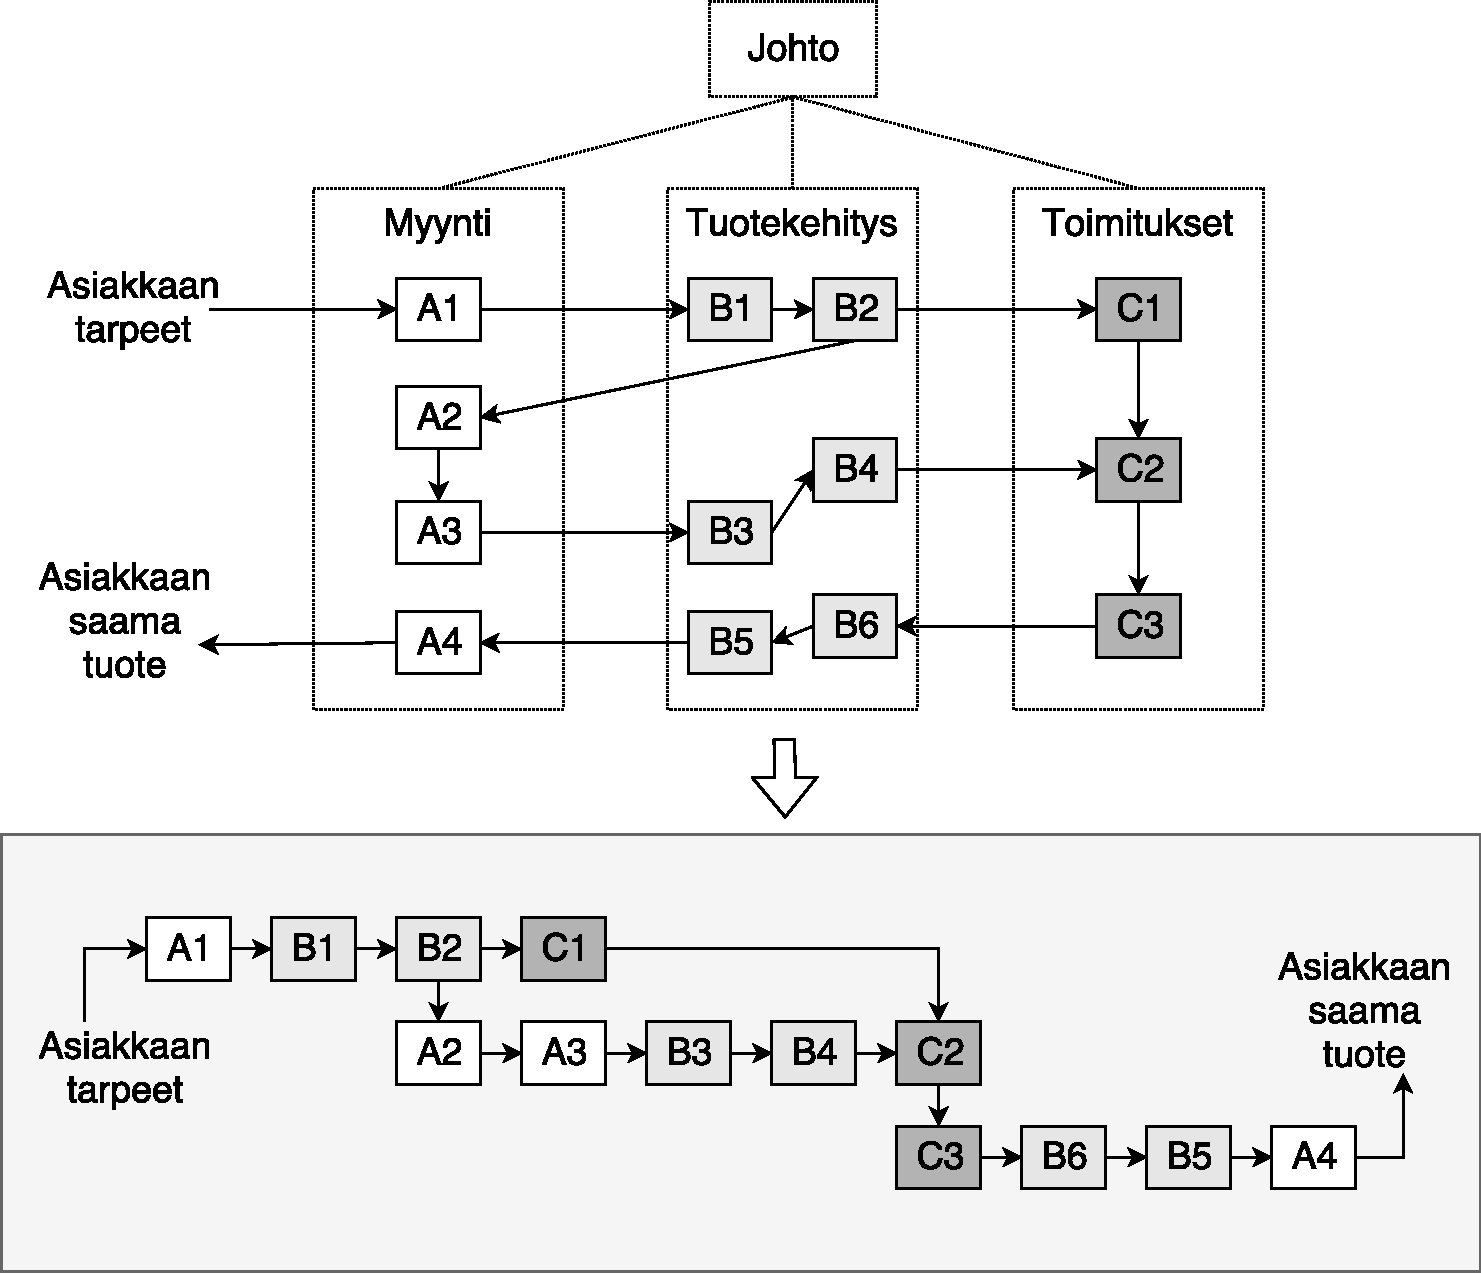
\includegraphics[scale=0.45]{images/Prosessikaavion.pdf}
    \caption{Esimerkki asiakasprosessista. \citep{ohjelmistotuotanto}}
    \label{fig:liikark}
\end{figure}

Kuvassa \ref{fig:liikark} on kuvitteellisen yrityksen asiakasprosessi. Liiketoimintaprosessi synnyttää näin tuotteen asiakkaalle kulkemalla läpi yrityksen eri toimintojen. \cite{ohjelmistotuotanto} tähdentävät, että liiketoiminnan ydinprosessit tuottavat arvoa ulkoiselle asiakkaalle, ja ovat siten tärkeässä roolissa yrityksen tavoitteiden saavuttamisessa. Ydinprosessien apuna on erilaisia tukiprosesseja, joissa asiakas onkin yrityksen sisäinen. Tälläisiä tukiprosesseja on esimerkiksi sisäisten tietojärjestelmien ylläpito tai sisäinen viestintä. \cite{okaytannot} sanovatkin, että liiketoiminnan tukiprosessit eivät välttämättä tuota ydinprosesseihin verrattavaa arvoa, mutta kun ne lakkaavat toimimasta, niillä on huomattavia vaikutuksia yrityksen toimintaan. \citeauthor{okaytannot} huomattavatkin, että liiketoimintaprosessilla on aina asiakas (joko sisäinen tai ulkoinen), joka saavuttaa prosessin avulla haluamansa lopputuloksen. Liiketoimintaprosessi siis ylittää organisaation rajat ja sillä on usein vähän riippuvuutta itse organisaation rakenteeseen.

\cite{leanit} kertovat, että Lean-johtamismallissa liiketoiminnan eri toiminnoista koostuvaa prosessinäkymää kutsutaan arvovirraksi. Heidän mukaansa Lean-johtamismallissa tavoitellaan näkyvää arvotuotannon järjestelmää ja alajärjestelmiä, jolloin huomio voidaan keskittää arvoa tuottamattomien vaiheiden poistamiseen. Arvovirran muodostamassa järjestelmässä muokataan sisään tulevia syötteitä tavoitteen mukaisiksi lopputuloksiksi sen sisältämien prosessien avulla, ja nämä prosessit vaativat, että yritys hankkii ja kuluttaa resursseja. Orzenin ja Paiderin mukaan tyypillisiä yrityksen resursseja ovat esimerkiksi aika, raha, raaka-aineet ja työvoima. He tähdentävät, että se miten yritys päättää järjestää arvoketjun toiminnot ja hallita sitä, määrää tuotannosta aiheutuvat kustannukset ja tuotot. Heidän mukaansa tavoitteena on tehokas arvovirta, joka kuluttaa mahdollisimman vähän resursseja parhaan mahdollisen lopputuloksen aikaansaamiseksi. Orzen ja Paider lisäävät, että toimivan arvovirran laatu on aina mitattavaa ja poikkeamat havaitaan nopeasti prosessin aikana.

Haikalan ja Mikkosen \citeyearpar{okaytannot} mukaan prosessin laadulla ei tarkoiteta ekplisiittisesti hyvää laatua, vaan kontrolloitua laatua valittujen laatutekijöiden perusteella. Kilpailussa markkinoilla korostuu yrityksen valitsemat laatutekijät, koska tuotteiden ja palveluiden laatu rakentuu toimintaprosessien laadusta \citep{ohjelmistotuotanto, teollisuustalous}. \cite{okaytannot} alleviivaavat, että uutta laatutekijää on liki mahdoton lisätä jo rakennettuun ohjelmistotuotteeseen tai -palveluun jälkikäteen, ja sen vuoksi halutut laatutekijät täytyy ottaa huomioon asiakasprosessin kehityksessä. \cite{ohjelmistotuotanto} kertovat, että laatutekijät valitaan mittaamaan liiketoiminnan tavoitteiden toteutumista asiakasprosessin tuloksena. Yrityksen määritelmä laadusta, jolla tavoitteet saavutetaan, antaa suunnan miten arvotuotannon toimintaa johdetaan ja kehitetään. 



\subsection{Ohjelmistotuotannon liiketoimintaprosessit}

Kuten \cite{teollisuustalous} kertoivat, tuotteiden ja palveluiden laatu rakentuu yrityksen toimintaprosessien laadusta, ja tämän periaatteen mukaan laatu pitää suunnitella ja rakentaa yrityksen toimintaprosesseihin. \cite{ohjelmistotuotanto, devops} mukaan ohjelmistotuotannossa työprosessien laatu korostuu erityisesti sen vuoksi, koska työprosessien toiminta on suurilta osin näkymätöntä, eikä laatua voi lisätä ohjelmistoihin tai järjestelmiin jälkikäteen. \citeauthor{devops} jatkaakin, että ohjelmistotuotannossa laatua mittaava ja palautekontrollin sisältävä komponentti on sisällytettävä työprosessin eri vaiheisiin. \cite{okaytannot} mukaan tehtäessä ohjelmistoja korostuukin hyvät toimintatavat, jotka on määritetty tuottamaan tavoitteen mukaista laatua. \cite{ohjelmistotuotanto} sanookin, että prosessikehityksen näkökulmasta onkin haaste tehdä ohjelmistotuotannon työprosessien vaiheista riittävän näkyviä, jolloin prosessin eri vaiheita voidaan seurata ja arvioida niiden tehokkuutta.

\cite{ohjelmistotuotanto} mukaan ohjelmistotuotannon pääprosessi on asiakasprosessi, jota tukevat tuotekehitys- ja ylläpitoprosessi. Liiketoimintamalli vaikuttaa oleellisesti miten nämä prosessit tukevat toisiaan. \citeauthor{ohjelmistotuotanto} jakavat asiakasprosessin kolmeen eri liiketoimintamalliin, täysin asiakkaan tarpeiden pohjalta rakennettava ohjelmisto tai suoraan "hyllyltä" asiakkaalle myytävä ohjelmistotuote tai palvelu. Näiden kahden ääripään välimaastossa on niin kutsuttuihin ohjelmistoalustoihin tai ekosysteemeihin perustuva malli, jossa asiakkaalle paketoidaan ohjelmistotuote tai palvelu olemassaolevista ja räätälöidyistä komponenteista. Ohjelmistotuotantoprosessi voidaan nähdä yhtenä asiakasprosessina, johon tuotekehitys ja ylläpito kuuluvat. Kuvassa \ref{fig:asiakasprosessi} on kuvattu asiakasprosessit eri liiketoimintamalleissa.

\begin{figure}[!h]
    \centering
    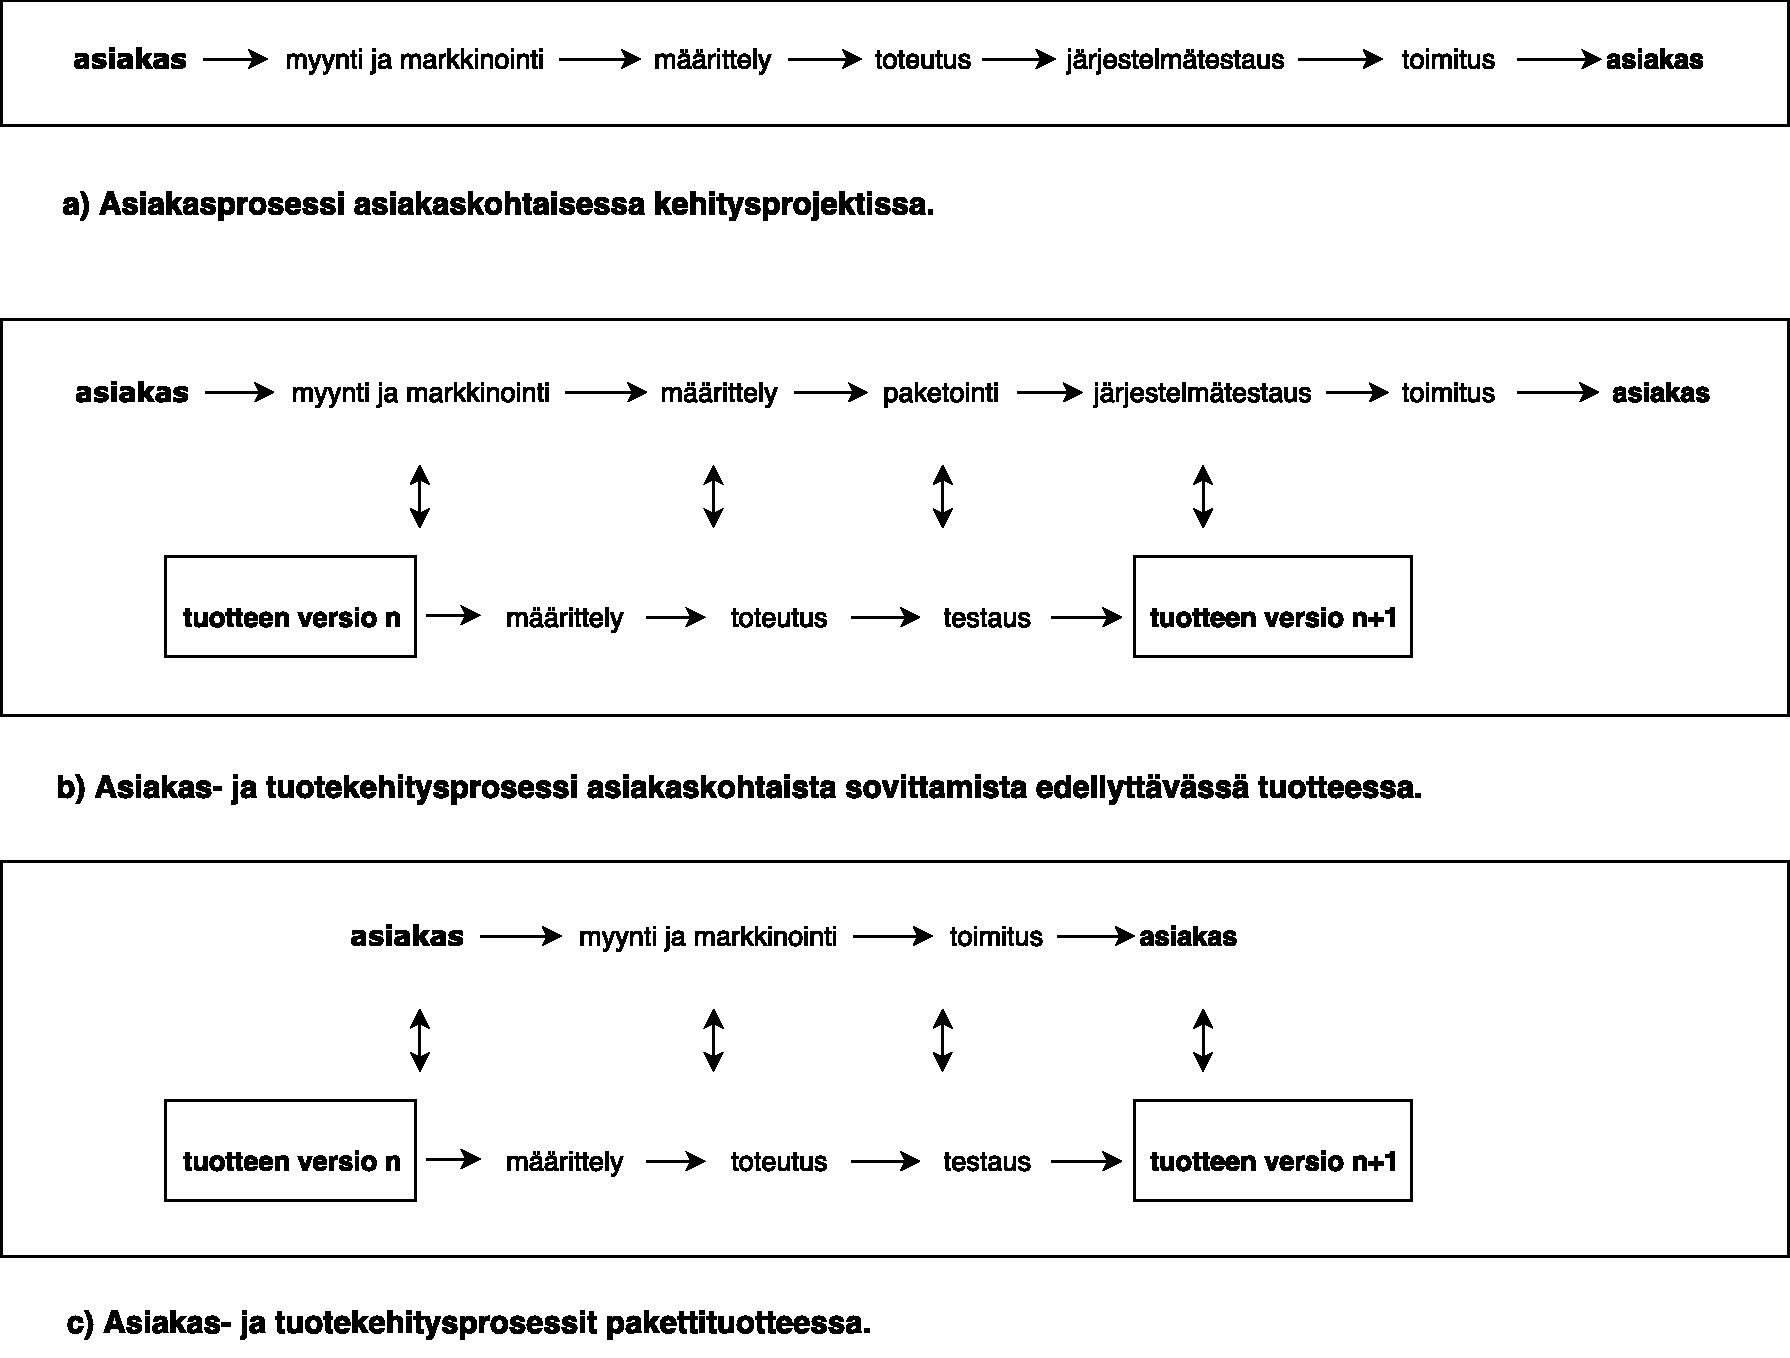
\includegraphics[scale=0.45]{asiakasprosessi.pdf}
    \caption{Asiakasprosessit eri liiketoimintamalleissa \citep{ohjelmistotuotanto}.}
    \label{fig:asiakasprosessi}
\end{figure}

Haikalan ja Marijärven mukaan on yleistä, että ohjelmistoyrityksen liiketoimintamalli sijoittuu kuvan \ref{fig:asiakasprosessi} a- ja c-liiketoimintamallien väliin. Tällöin tuotekehitys tuottaa perusmallin tuotteesta, joka paketoidaan asiakkaan toiveiden mukaan. Paketoinnilla tarkoitetaan ratkaisun kokoamista olemassa olevista komponenteista esimerkiksi konfiguroimalla. Paketointi voi myös sisältää asiakaskohtaisia muutoksia tai lisäyksiä, jolloin toiminta muuttuu asiakasprojektiksi. Yleisesti toimintaa tehostaakseen yritys pyrkii luomaan tuotteen joka on samanlainen asiakkaasta riippumatta. Usein todellisuus kuitenkin on, että asiakkaiden tarpeet vaihtelevat niin paljon, ettei asiakaskohtaiselta räätälöinniltä voi välttyä. Räätälöinnin määrää on kuitenkin hallittava, ja sen vuoksi tuotekehallinnan on oltava mukana asiakasprosessissa.

\cite{okaytannot} toteaa tuotteenhallinnan vastaavan tuotekehitysprosessista. Heidän kertovat ohjelmistotuotteiden koostuvan useista erilaisista komponenteista ja niiden erilaisista variaatioista, jotka kehittyvät tuotteen elinkaaren aikana. Ohjelmistotuotteen versio koostuu määrätystä komponenttien kokoelmasta. Tuotteenhallinta on tukitoiminto, jossa määritellään näihin asioihin liittyvät toimintatavat ja menetelmät. 

Tuotehallinta on yksinkertaisimmillaan silloin kun ohjelmistotuotteessa olevien variaatioiden määrä on pieni. Tällöin tuotteenhallinta on pääasiassa versionhallintaa, jonka tarkoituksena on helpottaa työskentelyn koordinointia tuotekehityksen aikana. Monimutkaisimmillaan tuotteenhallinta on silloin kun tuotteen konfiguraatio vaihtelee toimintaympäristöstä riippuen ja jatkokehitettävien komponenttien määrä on suuri. Jos tuotteessa on lisäksi asiakaskohtaisia sovituksia, tuotteenhallinta monimutkaistuu entisestään. \citep{okaytannot}

Asiakaskohtaista räätälöintiä vaativissa asiakasprojekteissa asiakasprosessi monimutkaistuu, koska tarvitaan erillinen määrittely-, toteutus- ja testausvaihe. Projektit vaativat myös resurssien, aikataulujen ja tehtävien määrittämistä, joita kaikkia on usein vaikea tuntea tai huomata etukäteen. Käytännössä yllättävien suunnittelemattomien tehtävien määrä voi olla jopa neljännes projektin tehtävistä sen päätyttyä. Onkin tavallista, että ohjelmistoprojektit ylittävät aikataulun ja budjetin epärealististen ennakkoarvioiden ja muuttuvien vaatimusten vuoksi. \citep{okaytannot}

Usein ongelma on historiatiedon puute vastaavista projekteista. Historiatiedon kerääminen vaatii organisaatiossa hyvin toimivaa laatujärjestelmää ja pedanttia toimintaprosessien nuodattamista, joka on usein mahdoton saavuttaa asiakaskohtaisesti muuttuvissa prosessimalleissa. Kirjoittajat esittävät, että on paradoksaalinen tosiseikka, että kaupan saa se joka on arvioinut projektin kustannukset ja valmistumispäivän eniten alakanttiin. Vaikka asiakasprojekteihin liittyykin ennalta odottamattomia asioita, ei toimintaprosessien laadusta kannata tinkiä. \citep{ohjelmistotuotanto, okaytannot}

Ohjelmistotuotteen elinkaaren kannalta suurimmat potentiaaliset säästöt ovat saavutettavissa ohjelmiston ylläpitokustannuksia pienentämällä. Tässä korostuu huolellisen suunnittelun ja ajan tasalla olevan dokumentoinnin merkitys. Usein tuotantoprosessista läpi päässeen laatuvirheen aiheuttamat kustannukset kertaantuvat ylläpitovaiheessa moninkertaiseksi. Laadunohjauksen keskeisimpiä tavoitteita onkin virheiden ennaltaehkäisy. Koska virheiden tekemiseltä ei voida kokonaan välttyä, virheet on pyrittävä poistamaan järjestelmästä mahdollisimman aikaisessa vaiheessa, jolloin kerrannaisvaikutuksilta vältytään. Näin vähenee sekä virheiden korjailun (rework) aiheuttama lisätyö kehitysprojektissa että käyttöönoton jälkeen tapahtuva ylläpitotyö. \citep{ohjelmistotuotanto}

Jalosta kappale Scrum-mallilla:
Projektin alkuvaiheessa on vaikea tehdä rationaalisesti perusteltuja lopullisia ratkaisuja, eikä projekti voi siksi edetä alussa määritetyllä oppikirjan mukaisella prosessimallilla. Projektin alussa saadut vaatimukset muuttuvat usein projektin edetessä, ja niihin liittyvät realiteetit selviävät vasta toteutuksessa kokeilemalla. Vaikka realiteeteista olisikin hyvä käsitys alkuvaiheessa, on ihmisryhmän vaikea kollektiivisesti käsitellä niitä virheettömästi. Yksilön on helppo tarttua jo oppimaansa ratkaisuun ja siksi realiteetin vaatima toimintamalli saattaa jäädä huomaamatta. Myös jo olemassa olevien ratkaisujen uudelleenkäyttö johtaa joskus omituisiin ratkaisuihin. Näistä ongelmista huolimatta tulisi pyrkiä rationaalisen prosessimallin mahdollisimman tarkkaan seuraamiseen, koska se antaa ohjeita mitä missäkin vaiheessa pitäisi tapahtua. Tällöin projektien prosessit saadaan muistuttamaan toisiaan ja opitaan muokkaamaan niitä sopivalla tavalla tarkoituksen mukaisiksi projektin aikana, jolloin projektin suunnittelu ja seuranta on ulkopuolisenkin näkökulmasta helpompaa. Ongelmat ohjelmistotuotannossa kulminoituvat toimintaprosessin aikaisiin inhimillisiin virheisiin.\citep{ohjelmistotuotanto}

Hyvän laatujärjestelmän yksi tavoitteista onkin estää inhimilliä erehdyksiä. Inhimillisten erehdysten estäminen raskastekoisella ja monipuolisia laatustandardeja valvovalla prosessilla ei useinkaan ole paras ratkaisu. Ohjelmistojen ja järjestelmien kanssa työskentelevillä ihmisillä on usein tapana suhtautua epäilevästi kankeisiin prosesseihin, ja sen johdosta ketterät menetelmät ovat kasvattaneet suosiotaan vastareaktiona kankealle prosessille. Hyvä työprosessi ohjelmistotuotannossa onkin mahdollisimman kevyt hallittavissa oleva prosessi. Ohjelmistotuotannossa hienoinkaan prosessi ei nimittäin korvaa tekijöiden ammattitaitoa. On kuitenkin täsmennettävä, että ohjelmistotuotannon ammattilainen tehtävään soveltuvan prosessin kanssa päihittää aina toisen ammattilaisen, jolla ei ole hyvää prosessia. Ongelmaksi muodostuu juuri sopivan prosessin rakentaminen. \citep{okaytannot}

Sen vuoksi uuden prosessin rakentamista uudelleen jokaista asiakastomitusta varten tulisi välttää. Prosesseille voi toki kohdistua hyvinkin erilaisia vaatimuksia tilanteesta riippuen. Laadunhallinnan järjestelmän tulisikin tarjota valmis pohja prosessille, joka tarjoaa sopivasti taipuvan rakenteen erilaisten tavoitteiden saavuttamiseksi. Sopivan prosessin rakentaminen onkin aina kompromissi. Käytäntö on osoittanut, että prosessimallin noudattaminen ja sen toimintaan liittyvän mittatiedon kerääminen on mahdollista ja järkevää. Se mahdollistaa toiminnan kehittämisen todelliseen historiatietoon perustuen. Tämä tietysti edellyttää että toimintaprosessiton suunniteltu sillä tavalla järkeviksi, että ne ovat noudatettavissa. Amerikkalainen Victor Basili on esittänyt helpon tavan todeta tuotantoprosessin sopimattomuus: se paljastuu projektin kohdatessa ongelmatilanteen. Jos ongelmatilanteessa ensimmäiseksi unohdetaan tuotantoprosessin mukainen toiminta ja ryhdytään kiireesti tekemään asioita ad hoc-tavalla niin todennäköisesti yrityksen tuotantoprosessi tulisi uusia. \citep{ohjelmistotuotanto}

Ohjelmiston kehittäminen poikkeaa muista tekniikan aloista abstraktin luonteensa takia. Ohjelmistotekniikassa on myös huomattavasti vaikeampi hahmottaa rakennettavan asian koko ja monimutkaisuus. Toinen ero ohjelmistotekniikassa konkreettisiin tekniikan aloihin on tuotantotyön ja tuotantotyöläisten puuttuminen; ohjelmistojen rakentamiseen liittyvä työ on suunnittelutyötä. Ohjelmistokehityksessä pääosissa on suunnittelu, jossa formaalilla tavalla kerrotaan tietokoneelle mitä sen pitää tehdä. Ohjelmointi sekä työkalujen käyttö ja konfigurointi on suunnittelutyötä. Formaalin suunnitelman eli ohjelman muuttamisen lopulliseksi ajettavaksi järjestelmäksi hoitaa tietokone suunnittelijan formaalien ohjeiden mukaan. Kehittämiseen liittyy olennaisena osana kehitysympäristön työkalujen, ohjelmistojen ja palvelinten valitseminen ja näiden asentaminen. Ensimmäistä kertaa tehtäessä tämä on ilman muuta suunnittelutyötä, mutta toistuessaan voi muodostua rutiiniksi. Tietotekniikassa on se mukava puoli, että kaikki rutiinit voidaan ja pitää automatisoida, niin tämäkin. Ympäristö on kuitenkin standardoitu ja tärkeimmiltä osiltaan samanlainen kaikkien kehittäjien kesken. kaikki järjestelmän asennukset kaikkiin ympäristöihin että ympäristöjen asennukset tapahtuvat automaattisesti ilman manuaalisia toimenpiteitä. Kaiken pohjana on sama suunnittelutyö, joka suurimmalta osalta on tehty jo kehitysympäristön ja ensimmäisen testiympäristön synnyttyä. Oleellista on, että myös tuotantoympäristöä koskee sama automatiikka kuin muita ympäristöjä. Järjestelmän tuotantopäivitys on yhtä kevyt operaatio kuin päivitys testiympäristöön. Tuotantoprosessin automatisointi on arkipäivää ja rakennettavissa nykypäivänä yleisesti käytössä olevilla työkaluilla. Automatisoidun tuotantoprosessin suunnittelu vaatii työtä ja osa työstä on rakennettavasta järjestelmästä riippuvaista. Aivan pienessä projektissa tuotantoprosessin täydellinen automatisointi ei välttämättä maksa itseään takaisin, mutta niissäkin tärkeimmät osat pitää ehdottomasti automatisoida. \citep{kallio}

Scrum asiaa?

Ohjelmistotuotannossa tavoitellaan ketterää, luotettavaa ja turvallista tuotetta. Kuitenkin käytännössä näiden kaikkien saavuttaminen on haastavaa. Usein tuotantoprosessia on vaikea määritellä ja mitata, jolloin prosessin hallitseminen on haastavaa. 

vaikeasti määriteltävissä olevat tuotantoprosessit, vaikeasti määriteltävissä ja mitattavissa olevan laatukomponentin puuttuminen, tuotanto- ja kehitysympäristön erot nostavat ylläpitokustannuksia 

Ohjelmistojen koko ja monimutkaisuus usein kasvavat liian nopeasti, jolloin menetetään tuotannon ketteryys. Tuotantoprosessia on vaikea määritellä ja siten mitata, koska ongelmat pyritään ratkomaan ketterästi. Joskus vaatimusmäärittelyssä ei osata kuvata todellista ongelmaa, joka halutaan ratkoa. 

\subsection{Liiketoimintaprosessien kehittäminen ohjelmistotuotannossa}

\textbf{Business process management - Prosessijohtaminen}

\cite{gandhi}
Business process management (BPM) is a discipline involving any combination of modeling, automation, execution, control, measurement and optimization of business activity flows, in support of enterprise goals, spanning systems, employees, customers and partners within and beyond the enterprise boundaries.\\

visualize – functions and processes\\
measure – determine the appropriate measure to determine success\\
analyze – compare the various simulations to determine an optimal improvement\\
improve – select and implement the improvement\\
control – deploy this implementation and by use of user-defined dashboards monitor the improvement in real time and feed the performance\\ information back into the simulation model in preparation for the next improvement iteration\\
re-engineer – revamp the processes from scratch for better results\\
This brings with it the benefit of being able to simulate changes to business processes based on real-world data (not just on assumed knowledge). Also, the coupling of BPM to industry methodologies allows users to continually streamline and optimize the process to ensure that it is tuned to its market need.

\textbf{DevOps}
\cite{devops}
DevOps and its resulting technical, architectural, and cultural practices represent
a convergence of many philosophical and management movements.
While many organizations have developed these principles independently,
understanding that DevOps resulted from a broad stroke of movements, a
phenomenon described by John Willis (one of the co-authors of this book) as
the “convergence of DevOps,” shows an amazing progression of thinking and
improbable connections. There are decades of lessons learned from manufacturing,
high reliability organization, high-trust management models, and
others that have brought us to the DevOps practices we know today.
Promo - Not for distribution or sale

DevOps is the outcome of applying the most trusted principles from the
domain of physical manufacturing and leadership to the IT value stream.
DevOps relies on bodies of knowledge from Lean, Theory of Constraints,
the Toyota Production System, resilience engineering, learning organizations,
safety culture, human factors, and many others. Other valuable
contexts that DevOps draws from include high-trust management cultures,
servant leadership, and organizational change management. The result is
world-class quality, reliability, stability, and security at ever lower cost and
effort; and accelerated flow and reliability throughout the technology
value stream, including Product Management, Development, QA, IT Operations,
and Infosec.
While the foundation of DevOps can be seen as being derived from Lean, the
Theory of Constraints, and the Toyota Kata movement, many also view DevOps
as the logical continuation of the Agile software journey that began in 2001.

The principles of Flow, which accelerate the delivery of work from
Development to Operations to our customers
• The principles of Feedback, which enable us to create ever safer
systems of work
• The principles of Continual Learning and Experimentation foster
a high-trust culture and a scientific approach to organizational
improvement risk-taking as part of our daily work

\subsection{Tavoitteena automaatio}

Monilla aloilla menestyksen perusedellytyksenä on tehokkaan automaation soveltaminen. 

Automaatiolla voidaan osittain korvata työvoimaa ja pienentää tätä kautta ksutannuksia. 
uusien teknologioiden kehitys myös edesauttaa automaation yleistymistä.
perustellaan usein myös käyttöasteiden nostamisella, automaattinen jåärjestelmä tekee töitä 24/7.
Automaattisissa järjestelmissä virheiden määrä on pienempi, kuin ihmisten vastaavassa työprosessissa.
Jotkut prosessit myös vaativat tarkkuutta, joka edellyttää tietokoneohjattua käyttöä.

\cite{groover} määrittelee automaation olevan koneellinen työkalu ihmisten aikaisemmin suorittamiin tehtäviin, ja yhä enemmän tehtäviin jotka olisivat muuten mahdottomia. Tällä hän tarkoittaa koneiden integroitumista järjestelmäksi, joka kykenee toimimaan itsenäisesti ilman ihmisen väliintuloa. Hänen mukaansa automaattinen järjestelmä suorittaa prosessia sen saamien tarkkojen ohjeiden mukaisesti, ja ohjeiden noudattamista valvoo palautekontrolli, jonka tehtävä on validoida järjestelmään tulevien syötteiden oikeellisuus ja valvoa ohjeiden noudattamista prosessin aikana. 

Lähes jokaisessa yrityksessä liiketoiminta on riippuvainen tietojärjestelmistä ja niiden kehittämisestä liiketoimintavalmiuksien kasvattamiseksi. Prosessijohtamisen näkökulmasta haaste on tehdä näkyväksi tietojärjestelmiin liittyvät työprosessit. Tämä korostuu erityisesti ohjelmistotuotannon laadun johtamisessa. Perinteisessä teollisuudessa liiketoimintaprosessiin liittyvien työprosessien hallinta on viety hyvinkin pitkälle esimerkiksi Toyota Kata-filosofian edistysaskelien kautta. Liiketoimintaprosesseihin on näin pystytty rakentamaan laatu, turvallisuus ja ketteryys sisälle. 

Key elements to identify a process for automation: \cite{groover}

The process requires consistency across the organization
The process is repeatable
The process needs to be free from error, every time


Prosessin automatisoiminen tarkoittaa, että prosessiin tuleva informaatio on ennustettavaa ja että informaation perusteella olevat lopputulokset ovat selvillä.

https://devops.com/automation-versus-orchestration/ 
Se että ODI-prosessi on automaattinen tarkoittaa että se rakennetaan komponenteista joihin automaatio on rakennettu sisään. Esim. onko order-prosessi rakennettu automaatio laatukomponentti mielessä? Onko toimitusprosessi rakennettu automaatio mielessä? Onko laskutusprosessi rakennettu automaatio mielessä?
Onko meidän henkilökunta tilausten vastaanotossa 

Koska Amazonilla ei ollut logistiikkaosaamista tai olemassaolevaa rakennetta, se joutui löytämään reitin muulla tavoin, verkkokauppana jossa niitä ei tarvittu. Rakentamaan disruptiivisen ominaisuuden prosesseihinsa.


Se että joku asia voidaan automatisoida tarkoittaa sitä että se toistuu useita kertoja samalla tavalla. Se että jokin asia toistuu useita kertoja samalla tavalla tarkoittaa, että jokin tavoitteen mukainen toiminta on onnistutaan määrämuotoistamaan toistumaan aina samalla tavalla. Jokin asia on onnistuttu määrämuotoistamaan tarkoittaa mestarillista arvoa tuottavien toimenpiteiden havaitsemista. Se
 että tunnistetaana arvoa tuottavat toimenpiteet tarkoittaa työprosessien hyvää tuntemusta siitä mitä arvoa tuottava työ on. 

Excessive automation: Rather than eliminating or at least simplifying
wasteful processes, they are often automated, creating additional
layers of system complexity and increasing total cost of ownership.\citep{leanit}
 
 
 Toimintojen jakamiseen liittyvät suunnittelupäätökset määrittävät, missä määrin annettu työ, tehtävä, toiminta tai vastuu on automatisoitu, ja missä määrin ne on annettu ihmisen suoritettavaksi. (ISO)
 separate man from machine. https://www.lean.org/balle/DisplayObject.cfm?o=3161 

\subsection{Kappaleen yhteenveto}

Mihin asti tuote tukee automaatiota on keskeinen kysymys?

\section{Contact center ohjelmistotuotteena}
Kappaleen tarkoitus: Kuvailla contact centereiden luonne ohjelmistotuotteena, minkälaisen ongelman ne ratkaisevat + tulevaisuuden trendejä: Integraatiot, omnichannel, CCaaS.\\\\

\cite{ccgartner} kuvailevat contact center—infrastruktuuriin kuuluvan joukon tuotteita (välineitä, ohjelmistoja ja palveluita), joita tarvitaan puheluliikenteen ohjaamiseen ja erilaisen median välittäiseen. Tälläisiä ratkaisuja heidän mukaansa käyttävät erilaiset organisoidut kommunikaatiopalvelut. Kontaktit järjestelmässä voivat olla ihmisavusteisia tai automaattisia itsepalveluita, jotka käyttävät äänivalikoita ja puheentunnistusta. Kontaktilla viitataan Latva-Koiviston \citeyearpar{latvakoivisto} mukaan viestintään asiakkaan kanssa erilaisisten viestinnän kanavien kautta, joista tyypillisä esimerkkejä ovat: puhelin, Internet-sivut, sähköposti, pikaviestit, Web-chatit, sosiaalinen media ja mobiililaitteet.

Contact centerit vaativat useiden toimintojen, arkkitehtuurien ja palveluiden yhteistoimintaa, kertovat \cite{ccgartner}. Heidän mukaansa markkinoilla on kolmen tapaista arkkitehtuurista lähestymistapaa, yksittäisiä integroitavissa olevia täsmäratkaisuja, laajoja toimintoja tarjoavia sarjatuotteita ja palvelupohjaisia ratkaisuja. He lisäävät, että näitä ratkaisuja tarjotaan piirikytkentä perusteisena puhelinverkkoratkaisuna, IP-perusteisena ratkaisuna tai näiden kahden yhdistelminä. 

\citeauthor{bernier} mukaan Internet mullisti contact centereitä kahdella tavalla: Kontakteja voidaan käsitellä useassa eri lokaatiossa hajautetusti saman järjestelmän avulla, ja organisaation Internet-sivut tulivat asiakaspalvelun keskiöön. Aikaisempia kehitysaskeleita oli esimerkiksi CTI-teknologia, jolloin tietokoneella pystyi siirtämään tietoa puhelinverkkoon ja asiakaspalvelija pystyi käsitellä puheluita tietokoneen avulla. Internetin ja mobiililaitteiden myötä alettiin puhua monikanavaisesta asiakaspalvelusta, sanoo \citeauthor{bernier}. Hän lisää, että tämän jälkeen yritykset havaitsivat ettei pelkän puhekanava riitä contact center-toiminnoissa. 

Contact center-ratkaisu ja siihen liittyvä arkkitehtuuri hankitaan tavallisesti yksittäiseltä toimijalta, koska ratkaisun hallinta on tällöin yksinkertaisempaa ja integraatiomahdollisuudet ovat laajempia, kertovat \cite{ccgartner}. Siksi isoissa hankkeissa suositaankin johtavien toimittajien kokonaisratkaisuja, jotka käsittävät toimittajien omia ja strategisten kumppaneiden ratkaisuja. \cite{bernier} kertookin, että itse contact center on vain puolet kokonaisratkaisusta, koska ratkaisun hyöty rakentuu integraatioista muihin yrityksen järjestelmiin, kuten asiakastiedon- ja työnkulunhallintaan.

\subsection{Teknologinen näkökulma} 

Perinteisiä asiakaspalvelujärjestelmän komponentteja ovat automaattinen puheluiden jakelu (ACD), tietokoneen ja puhelinliikenteen integraatio (CTI), äänivalikko (IVR), ennustava puheluiden valinta (predictive dialing), reaaliaikainen monitorointi, raportointi ja analytiikka.

Asiakaspalveluratkaisut ovat historiallisesti olleet luonteeltaan järjestelmiä, jotka on asennettu on-premises ratkaisuna yrityksen omaan konesaliin, kertovat \cite{vcc}. Tämä johtuu osittain siitä, että ne syntyivät aikana ennen Internettiä, jolloin kaikki liiketoiminnassa tarvittavat järjestelmät oli asennettava sinne missä liiketoimintaa harjoitettiin. Edelleenkin on asiakaspalvelujärjestelmä saatetaan osittain asentaa on-premises ratkaisuna, kertoo \cite{weiner}. Tällöin järjestelmä ja siihen liittyvä infrastruktuuri asennetaan yrityksen omaan konesaliin, ja yritys tai kumppani vastaa ylläpidosta. Etuna yrityksen näkökulmasta on kontrolli integroituihin järjestelmiin, niiden sisältämään dataan ja kustomointi omien tarpeiden mukaan. Selkeä haitta on isot investointikustannukset, ja rajoitetut mahdollisuudet integraatiolle ja tyypillisesti palvelutaso on heikompi kuin virtuaalisesti tuotetussa ohjelmistopalvelussa. 

\cite{vcc} olivat jo vuosia sitten eri mieltä. He näkivät jo silloin, että tulevaisuus on monikanavainen ja siksi on-premises asiakaspalvelujärjestelmän ei ole mahdollista tuottaa investointia takaisin. Syynä tähän oli heidän mukaansa se, että on-premises ratkaisun toimintojen kehittäminen olisi liian iso kustannus, ja investoinnit tulisi kohdentaa virtuaalisen ohjelmistopalveluna tuotetun asiakaspalvelujärjestelmän toimintojen kehittämiseen Internet-teknologioiden avulla. Virtuaalisessa asiakaspalvelujärjestelmässä yritys maksaa palveluntarjoajalle kuukausittaista tai vuosittaista maksua palvelun ylläpidosta palveluntarjoajan konesalissa. Käyttöönotto vaatii tässäkin investointia, joka on pilvi- tai selainpohjaista ratkaisua kalliimpi. Agentti käyttää järjestelmää esimerkiksi puhelinverkon tai VoIP-teknologian avulla mistä tahansa lokaatiosta. Ainoa vaatimus on verkkoyhteys ja työasema tarvittavine sovelluksineen. Tämän ratkaisun heikkous on palveluntarjoajan rajaamat  mahdollisuudet integraatiolle, kustomoinneille ja versionpäivityksille, jotka vaativat usein lisäinvestointeja \citep{talkdesk}. Tämä SaaS-malli on ollut yleinen Suomen markkinoilla.

Asiakaspalvelujärjestelmiä toimitetaan myös pilvipalveluna, jolloin ratkaisu tarjotaan Internetin yli ohjelmistona tai selainpohjaisena ratkaisuna päätelaitteelle. Keskeinen hyöty pilvipalvelumallissa on multitenattisuus, jolloin käyttäjät jakavat palvelun resursseja ja ovat siten kustannustehokkaita palveluntarjoajan näkökulmasta. Tämän myötä myös palvelutaso on korkea, koska kaikki on kahdennettu. Kustannukset palvelun käyttöönotossa ja käytössä ovat huomattavasti muita pienemmät. Käyttöönottoon kuluva aika on myös minimaalinen sisältäen ainoastaan tarvittavat konfiguraatiot järjestelmään. Pilvipalveluissa hyötynä on myös se, että ne integroituvat dynaamisemmin muiden selain- ja pilvipohjaisten ratkaisujen kanssa ja ne ottavat tietoturvan, yksityisyydensuojan ja palvelutason parhaiten huomioon. Selainpohjaisissa ratkaisuissa suurin haitta on se että kaikki toiminnot tapahtuvat selaimessa, jolloin sen maailman rajoitukset ovat läsnä. \citep{talkdesk}

\cite{ccgartner} mukaan contact center-ratkaisut ovat perinteisesti olleet laitteistokeskeisiä, mutta yhä useammat toimittajat pyrkivät tuottamaan tuotteistettuja valmiiksi konfiguroituja perusratkaisuja, joihin on helppo integroitua. Keskeinen ajuri on tarjota erilaisia valmiita ratkaisukokonaisuuksia niiden hankkimisen, konfiguroinnin ja toimittamisen yksinkertaistamiseksi. Tämän vuoksi pilvipalvelupohjaiset Contact Center as a Service-ratkaisut nostavat suosiotaan. Pilvipalvelumallin tehokas hyödyntäminen contact center-ratkaisuissa on mahdollistanut sen, että yhä pienemmät yrityksen voivat ottaa ratkaisun käyttöön kustannustehokkaasti. Esimerkiksi Amazon tarjoaa tälläistä palvelua niin sanottuna Serverless-palveluna, jossa kustannus perustuu toteutuneeseen palvelun käyttöön.

\subsection{Contact centerin rakentaminen}

Kuvaus lähtökohdista erilaisille asiakkaille. Koska muodostuu asiakasprojekteja ja koska on mahdollista ottaa käyttöön nopeasti.
aspa
\subsection{Tulevaisuus}

Jatkossa yrityksen luovat uusia digitaalisia palveluita asiakaskokemuksen kehittämiseksi. Tämä ennen kaikkea muuttaa tapaa jolla palveluita tuotetaan ja siten myös asiakaskohtaamiset muuttuvat. Automaattiset itsepalvelukanavat ovat contact centeriin verrattuna halvempia ylläpitää, ja contact centerin ongelmana on ollut asiakaspolun katkeilu ja siten sillä on ollut heikentävä vaikutus asiakaskokemukseen. Itsepalvelukanavien hyödyntäminen arkipäiväistyy monessa transaktiivisessa toiminnossa, ja agentti vapautuu enemmän arvoa luoviin tehtäviin. Asiakaspolun merkitys kasvaa tällöin ja siten siitä kerättävää dataa on hyödynnettävä, jotta tiedetään mitä asiakas haluaa hänen ollessa yhteydessä. Puhutaan saumattomasta asiakaskokemuksesta, jossa päästään lähemmäs intiimiä vuorovaikutusta, joka menetettiin siirrettäessä palveluita verkkoon. (deloitte)

Seuraavassa vaiheessa asiakkaat odottavat saumatonta vuorovaikutusta palveluntarjoajilta koska tahansa ja miten tahansa.
Asiakkaat haluavat asioida viestimällä ei soittamalla.
Chatbotit tekevät tuloaan.
Tekoälyn avulla tier 1 yhteydenotot vähenevät järjesstelmän älykkyys kasvaa tukitoiminnoissa.

\subsection{Kappaleen yhteenveto}

\section{Teknologiat automatisaation taustalla}
Kappaleen tarkoitus: Kuvailla miten digitaalista transformaatiota läpikäyvä yritys toimii, mitä tämä tarkoittaa operaattorin näkökulmasta ja mitkä teknologiat ovat tässä tuomassa automaatiota. Relevantti koska Telia kohdentaa uusien teknologieoiden hyödyntämisen sen keskeisimpiin liiketoimintaprosesseihin. \\\\

Digitaalisten teknologioiden hyödyntäminen yrityksen liiketoimintaprosessissa alentaa liiketominnan käyttökustannuksia ja parantaa asiakaskokemusta  \citep{lamoureux, jungner}. Lamourexin mukaan yritykset, jotka omaksuvat uusien digitaalisten teknologioiden käytön liiketoiminnassaan, suoriutuvat markkinoilla kilpailijoitaan paremmin. Hän lisää, että digitaalinen transformaatio on yrityksille selviytymisen edellytys, ja kilpailukyky markkinoilla rakentuu relevanttien teknologioiden ja niiden mahdollistamien liiketoimintavalmiuksien tunnistamiseen ja rakentamiseen. 

Digitaalisuus ja siihen liittyvä automaatio ja robotiikka ovat termeinä haastavia, koska niiden merkitys jalostuu ajan kuluessa, eri ympäristössä ja yksilöiden mielissä. Ne myös kuvaavat monimutkaisia teknologisia edistysaskelia, joita on vaikea kuvata tyhjentävästi. Keskustelussa termit myös yksinkertaistuvat ja sekoittuvat toisiinsa. Onkin tärkeä muistaa, että juuri nyt niillä tarkoitetaan asioiden tekemistä aivan uudella tavalla, eikä vain automaation tai muun uuden teknologian käyttämistä nykyisissä prosesseissa. Mooren \citeyearpar{susanmoore} mukaan kyse on uuden arvon luomisesta, eikä vain parannuksista vanhaan. Hän täsmentää, että automaatio ei vähennä ihmistyön määrää, vaan ihmistyö kohdentuu luovien ratkaisujen tekemiseen teknologian avulla. Teknologia valjastetaan luomaan yksilöllistä arvoa ihmisille \citep{jungner, susanmoore}.

Digitaalisuus itsessään ei ole mikään uusi asia. Digitaalisten teknologioiden kehitys alkoi tietokoneen keksimisestä ja yleistymisestä. Internetin myötä tietokoneet ovat yhteydessä toisiinsa ja näin tieto on tarjolla paikasta ja ajasta riippumatta. Pilviteknologioiden myötä on mahdollista käyttää lähes rajaton määrä laskentatehoa ja tallennustilaa. Tietoliikenneyhteyksien kehittymisen myötä tietoa on mahdollista siirtää paikasta toiseen yhä nopeammin. Se mitä digitaalinen tarkoittaa, muuttuu edelleen kun aikaa kuluu. Tässä työssä digitaalisilla teknologioilla tarkoitetaan nimenomaan pilvestä saatavilla olevaa laskenta- ja tallennuskapasiteettia, sekä Internet-teknologioita, joiden avulla tietokoneet ovat yhteydessä toisiinsa. Tämä digitaalisuuden aalto on hyödyllinen monilla tavoin. 

Jungnerin \citeyearpar{jungner} mukaan hyötynä digitaalisuudessa on reaalimaailman asian muuttuminen tietokoneen ymmärtämään binäärimuotoon, jolloin tietokoneen laskentatehoa ja tallennustilaa voidaan käyttää todellisen maailman ilmiöiden seuraamiseen, ymmärtämiseen ja synnyttämiseen. Tällöin voidaan rakentaa työvälineitä mallintamaan reaalimaailman ilmiöitä tietokoneen maailmaan, siirtää reaalimaailman vuorovaikutusta tietokoneiden maailmaan ja avata tietokoneille tie toimia suoraan reaalimaailmassa. Teknologian kehitys mahdollistaa uusien toimintamallien syntymisen, joiden avulla yhä monimutkaisempia reaalimaailman asioita voidaan mallintaa tietokoneelle.

\subsection{Digitaalinen visio}

Lamourex \citeyearpar{lamoureux} kertoo, että yritys voi hyödyntää digitaalisen teknologian työvälineitä kehittääkseen tuotteita ja palveluita, tehokkaampia prosesseja ja asiakaskokemusta. Hänen mukaansa digitaalinen transformaatio tarkoittaa näiden osa-alueiden jalostumista digitaalisten teknologioiden avulla. Kaikkea ei kuitenkaan ole tarkoituksenmukaista digitalisoida kerralla, vaan jalostamisen tulisi hänen mukaansa aloittaa tunnistamalla teknologiat, joilla voidaan rakentaa liiketoimintavalmiuksia tärkeimpien pullonkaulojen ratkaisemiseen. Taulukossa \ref{tab:digkys} Lamourex esittää kysymykset, joihin digitaalisen vision antaa vastauksia.

\begin{figure}[!h]
    \centering
    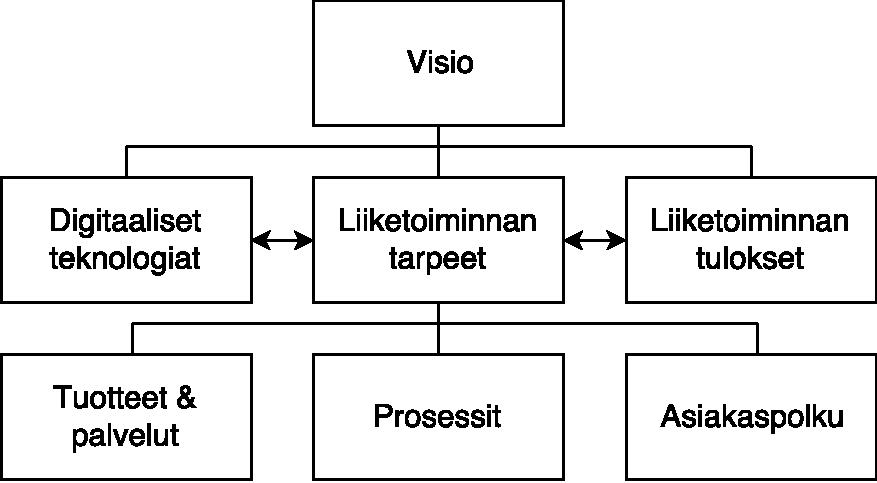
\includegraphics[scale=0.6]{images/digitaalinenvisio.pdf}
    \caption{Viitekehys digitaalisten teknologioiden hyödyntämiseen. \citep{lamoureux}}
    \label{fig:digivisio}
\end{figure}

Transformaation askeleet digitaalista visiota kohti, vaatii reaalimaailman toimintamallien arvoa tuottavan osan tunnistamista ja muuntamista tietokoneen luettavaksi, sekä arvotuotannon kehittämistä digitaalisen vision ehdoilla. Tämä vaatiikin reaalimaailmassa olevien toimintamallien pilkkomista, uudelleen järjestämistä ja eritoten karsimista \citep{leanit}. Suurin este transformaatiossa onkin organisaation vakiintunut tapa toimia, jolloin kulttuuriset näkymättömät tavat eivät sovellu digitaaliseen maailmaan \citep{jungner, lamoureux}.

MIksi transformaatio on relevantti? Sen avulla voi valjastaa digitaalisen tekemään työtä ja keskittyä luovaan asiakkaan ksilöllisseen palvelemiseen tjsp

Jungner \citeyearpar{jungner} kertoo tietokoneiden roolin korostuvan reaalimaailmassa, joka johtaa tehokkaampaan tapaan toimia. Monenlainen toiminta siirtyy tietokoneen suoritettavaksi. Tämän myötä kokonaiset toimialat uudistuvat ja myös koko yhteiskunta. Jungner käyttää esimerkkinä pankkialaa, joka käy läpi suurta muutosta, jossa palveluiden ylläpitäminen vaatii murto-osan siitä työvoimasta mitä aikaisemmin tarvittiin. Toisaalta pankkipalvelut ovat laajempia kuin aikaisemmin. Jungner alleviivaakin, että ei-digitaalisella tavalla toimiessa nykyinen pankkitoiminta vaatisi koko Suomen kansan työpanoksen. Lamourex \citeyearpar{lamoureux} korostaa, että
uusien teknologioiden hyödyntäminen ei ole vaihtoehto, vaan selviytymisen edellytys.

Jungner \citeyearpar{jungner} puhuu talouden ekosysteemin luovan tuhon kiihtymisestä nopeutuvan digitaalisuuden vuoksi, jossa vanhat yritykset, tuotteet, palvelut, tavat ja ammatit häviävät uusien tuottavampien sovellusten tieltä. Uusissa ammateissa työtavat muuttuvat hyödyntämään verkostoneituneita työvälineitä, ja tiedon hyödyntäminen tehostuu, jolloin innovaatioiden sykli nopeutuu. 

Lamourexin \citeyearpar{lamoureux} mukaan digitaalisten teknologioiden hienostuneisuus ja lukumäärä kasvaa innovaatioiden syklin nopeuduttua. Tämän myötä myös käyttötavat moninkertaistuvat. Uusien teknologioiden ja niiden käyttötapojen tehokkaalla hyödyntämisellä on mahdollista saada aikaan yhä isompia tuloksia, hän lisää. Pienet toimijat voivat vallata siivun markkinasta isommilta toimialan johtajilta tehokkaasti kohdennetulla ja ketterällä ratkaisulla. Lamourex \citeyearpar{lamoureux} puhuu disruptoinnista, jossa haastetaan vallitseva tila uudella radikaalilla tavalla, joka tuhoaa vanhaa ja luo uutta nopeasti. Hän tuo vahvasti esiin, että disruptointi ei ole vain pienten ja ketterien organisaatioiden yksinoikeus, sillä myös suuryritys voi disruptoida markkinoita. Usein suuryrityksellä onkin etulyöntiasema jos se tunnistaa nykyisten verkostojensa ja prosessiensa vahvuudet ja kykenee tekemään rohkeita kokeiluja uusien teknologioiden kanssa. 

Jungner \citeyearpar{jungner} pohtii, että puoliksi suunniteltu on digitaalisessa maailmassa tarpeeksi hyvin tehty. Hänen mukaansa käytännön kokeilut kumppaneiden ja asiakkaiden kanssa ovat nopein tapa selvittää mikä oikeasti toimii, eikä käyttää pitkää aikaa suunnitteluun. \citeauthor{devops} \citeyearpar{devops} on myös samaa mieltä: Maali liikkuu yhä nopeammin, ja siihen osuu varmemmin jos ampuu useammin ja pienemmissä erissä. Lamourex \citeyearpar{lamoureux} muistuttaa kuitenkin, että kokeiluja ohjaa digitaalinen visio uusien teknologioden tunnistaminen, joilla voi ratkaista liiketoiminnan tarpeita ja saada aikaan tuloksia. \citeauthor{gandhi} \citeyearpar{gandhi} mukaan ratkaisevaa on havaita, että digitaalinen investointi tuottaa arvoa vasta kun se on ratkaisuna tuottamassa arvoa. Kilpailussa ovat vahvoilla toimijat, jotka osaavat laittaa uudet ratkaisut työhön asiakkaiden ja muiden kumppaneiden kanssa.

\begin{table}[h!]
    \centering
    \begin{tabular}{l}
       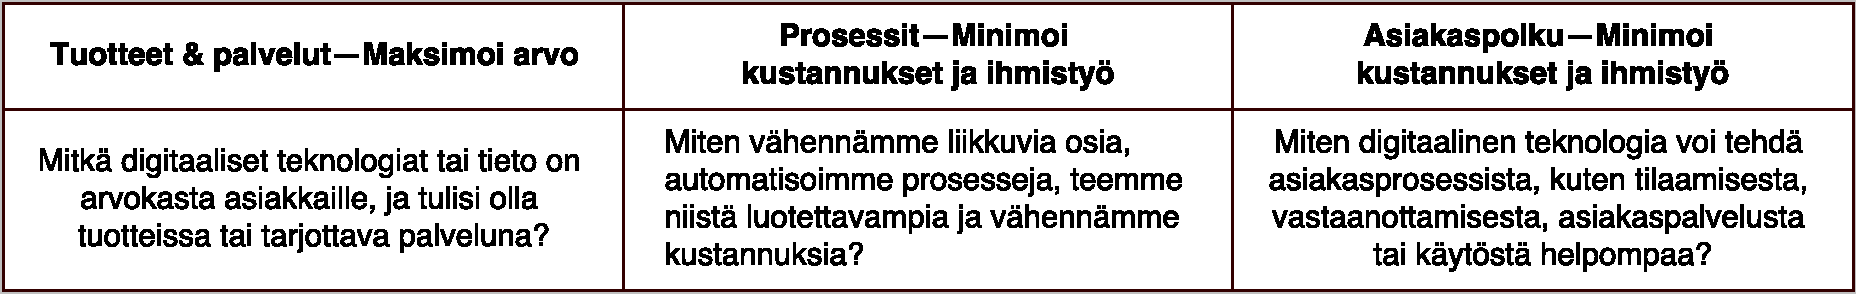
\includegraphics[scale=0.45]{images/priorisointi.pdf}
    \end{tabular}
    \caption{Kysymyksiä digitaalisen vision hahmottamiseen \citep{lamoureux}}
    \label{tab:digkys}
\end{table}

Lamourexin \citeyear{lamoureux} mukaan yrityksellä on kolme pääasiallista tapaa kehittää liiketoimintavalmiuksia markkinoilla: Kehitä tuotetta tai palvelua tekemällä siitä arvokkaampia asiakkaalle. Tehosta sisäisiä prosesseja tuottaaksesi arvo pienemmillä kustannuksilla. Paranna asiakaspolkua helpottamalla asiakkaan arvon hankkimista. Hänen mukaansa nämä osa-alueet on priorisoitava toimialan mukaan. Arvotuotannon kolme pääasiallista elementtia tuote, prosessit tai asiakaspolku korostuvat toimialan mukaan erottavana kilpailutekijänä. Investoinnit tulisi kohdentaa kilpailutekijän kehittämiseen tunnistetuille digitaalisilla teknologioilla.

Yrityksen näkökulmasta teknologialla parannetaan tuotteita, sisäisiä prosesseja ja asiakaskokemusta. Pelkästään teknologian käyttäminen ei kuitenkaan tuo hyötyä liiketoimintaan. Valitulla teknologialla täytyy olla potentiaalia kasvattaa kilpailukykyä määrätyssä aikajaksossa, ja investoinnin tulee ottaa riskit huomioon. Uusia teknologioita tulee ja menee, ja siksi tulisikin olla kykyjä tutkia useampia potentiaalisia teknologioita saman aikaisesti. Ajankohdan tulee myös olla sopiva, koska teknologiat saattavat vanhentua luultua nopeammin ja liian aikaisin tehty investointi uuteen teknologiaan saattaa heikentää kilpailuedun saamista. Teknologian hyödyntämisessä vaaditaan myös selkeä kuva liiketoimintavalmiudesta joka halutaan rakentaa sen avulla. Uusien teknologioiden käytön omaksuminen liiketoiminnan tavoitteiden saavuttamiseksi ei myöskään tapahdu itsestään. Teknologian käyttäminen kilpailuedun saavuttamiseksi markkinoilla onkin organisaation opittu taito. Eli organisaation sisäisten ja ulkoisten tavoitteen kannalta relevanttien sidosryhmien kyky tehdä yhteistyötä. Tämän kyky on vaikeampi rakentaa organisaatioissa, joissa tavoitteen kannalta relevantteja sidosryhmiä on useampia. Suurempi sidosryhmien määrä vaikeuttaa tiedon vaihtamista ja kommunikointia. Uuden teknologian hyödyntäminen kilpailiedun saavuttamiseksi vaatiikin toimintamallin muuttumista, usein yksinkertaisempaan suuntaan.

\subsection{Operaattorin digitaalinen transformaatio}

- Operaattori tekee päätöksiä ainakin osittain digitaalisen transformaation mukaan, joka ohjaa siis tekemistä. Mckinseyn raportti.\\
- Operaattoreiden haasteet muutosvoimissa

Vaikka kilpailu on ollut kovaa, perinteisesti operaattoriliiketoiminta on ollut suojassa uudelta kilpailulta, koska maantieteellistä markkinaa jakaa vain muutama operaattori. Tämä tilanne on pikkuhiljaa muuttumassa, ja operaattorit joutuvat kehittämään uusia liiketoimintamalleja vastatakseen uudenlaiseen kilpailuun. Operaattoreiden haasteet tiivistyvät kolmeen asiaan: \citep{inderes}
\begin{itemize}
    \item[] OTT-toimijat, kuten Skype ja Whatsapp, tarjoavat puhe- ja viestintäpalveluita, jotka syövät operaattoreiden tulovirtaa perinteisesti kannattavasta liiketoiminnasta.
    \item[] Kuluttajat käyttävät yhä enemmän erilaisia video- ja sosiaalisen median palveluita, ja tämän vuoksi operaattorit joutuvat investoimaan verkkokapasiteettinsa kasvattamiseen ja verkon laadun ja luotettavuuden parantamiseen. Näiden palveluiden käytöstä aiheutuu iso kuorma verkoille, mutta tuotot menevät suurelta osin OTT-toimijoille.
    \item[] Kuluttajat ja yritykset ovat yhä enemmän hintatietoisia ja vaativat parasta hinta/laatu-suhdetta verkkopalveluiltaan.
\end{itemize}

Nämä kolme asiaa heikentävät ydinliiketoiminnoista tulevaa liikevaihtoa samalla kun tarve investoinneille kasvaa. Tämän vuoksi raskas organisaatio- ja kulurakenne tuo ongelmia hintakilpailussa. Ketterät OTT-toimijat pelaavat pitkälti omilla säännöillään, kun operaattorin toimintaa rajoittaa tiukka sääntely. Perinteisesti operaattoreiden vanha IT-infrastruktuuri on myös hyvin kompleksista, joka hidastaa toimintaa. \citep{inderes}\\

Operaattori voi lähestyä tätä ongelmaa eri tavoin. Yksi strategia on keskittyä ydinliiketoimintaan ja tuottaa yhteyspalveluita mahdollisimman hyvin ja kustannustehokkaasti. Toinen strategia on vastata OTT-kilpailuun tarjoamalla omia vastaavia palveluita ja laajentua media- ja sisältö liiketoimintaan. \citep{inderes}


\subsection{Teknologiat digitaalisessa transformaatiossa}
Ns. työkalupakki jonka teknologiat tarjoavat.
Digitaalisen teknologian myötä automaatio on scriptausta apeja jne pilvessä jne. Kaikki on avointa: data, rajapinnat

Digitalisaation työkalupakki(aoit, rpa, ...)
Digitalisaation menetelmät (devops, lean, kaikki on avointa...)
Muutosvoimat operaattorin näkökulmasta(doing digital right)



teollisuudessa disruptioitiin ja sitten lähti muutos leaniin.
Automaatio ja DevOps tulee täällä. Tämän vuoksi jne.

Multi-single asiaa myös


\subsection{Kappaleen yhteenveto}

\clearpage

\section{Tutkimusmenetelmä}

Kun kysyn miksi tätä prosessia ei ole automatisoitu, koostuu vastaus kahdenlaisista elementistä: Ympärillä olevat toimintamallit estävät tavoitteisiin johtavan työn tekemisen aikataulussa, jolloin ei päästä tekemään ja analysoimaan miten automaatio rakennetaan. Komponentit, jotka ovat valittavissa prosessin rakentamiseen, eivät tue automaation rakentamista halutulla tavalla, jolloin jää manuaalisia työvaiheita.

Tässä tutkimuksessa valittiin laadullinen lähestymistapa ymmärtämään/arvioimaan miksi asiakasprosessin automatisoinnissa ei ole toistaiseksi onnistuttu vertaamalla asiakasprosessin rakentamisessa käytettyjen toimintamallien ja järjestelmäkomponenttien sopivuutta suhteessa liiketoiminnan tavoitteisiin, kun tavoitteena on rakentaa automatisoitu asiakasprosessi. Arvioinnissa otetaan huomioon, että kyseessä on operaattorin contact center-liiketoiminta, ja operaattorin uudet investoinnit painottuvat digitaaliseen transformaatioon. 

Tämän lisäksi pyritään ymmärtämään syitä toimintaympäristössä liiketoimintatavoitteiden taustalla. 

Aineistopohjaisen teorian rakentaminen (grounded theory building)\\
- Menetelmässä kehitetään teoriaa ilmiöstä aineistosta löytyvien havaintojen, niiden koodauksen ja järjestämisen kautta.\\
- Teoria perustuu aineistoon, jota voidaan hankkia kenttätyössä haastatteluin ja havainnoin sekä dokumenteista.\\
- Toimii tässä tilanteessa koska nykyiset tavoitteet ovat ristiriidassa toteutuneiden asioiden kanssa, ja tilanne vaatii selvittämistä.\\
- Nykytilan havaitsemisella voidaan antaa teorian pohjalta tapoja edetä tavoitteeseen\\

\subsection{Tutkimussuunnitelma}

Single Case study: Tapaustutkimuksessa käsitellään yksittäistä, rajattua kokonaisuutta luonnollisessa ympäristössään, ja kuvaillaan tutkimuskohteen ominaispiirteitä tarkasti ja totuudenmukaisesti. Tutkittavat tapaukset ovat ainutkertaisia, ja niitä tutkitaan omassa erityisessä ympäristössään. Eli kuvataan prosessin rakentamista, jossa kolme osaa: toimija, toimintamalli tai metodi ja komponentti/työkalu.

Toiminnan nykytilan havaitseminen suhteessa tavoitteisiin:\\
- Kontakti L asiakasprosessin rakentamisen tila\\
- Kontakti M asiakasprosessin tavoitteet suhteessa toteutettuun\\
- VIP-tuotteen asiakasprosessin rakentaminen\\
- Merex-tuotteen asiakasprosessin rakentaminen\\
+ Prosessikuvaukset\\
- Miten toteutetut asiakasprosessit kehittyivät tämän jälkeen?\\
- Pasi Savilaakso, prosessivastaava (asiantuntija)\\
-> Toiminnan nykytilan havaitseminen suhteessa tavoitteisiin\\

Kontakti L-asiakasprosessiin valittavien komponenttien automatisointimahdollisuudet asiantuntijahaastatteluina\\
- Zylinc: Cloudy tiimi yritti 6 viikkoa onnistumatta\\
- Tilaus: Claudia/Salesforce, yritysportaali, Eshop (Transformaatio)\\
- Laskutus: Komarc Multibella (Transformaatio)\\
-> Valittavissa olevien komponenttien tuki automatisoinnille, ja sen mahdollistava teknologia (tarvitaanko robitiikkaa?)\\

Itsepalvelu: Asiantuntijahaastatelu\\
- Tilausvaiheen itsepalvelu\\
- Ylläpitovaiheen itsepalvelu\\

Robotiikka:\\
- Kustannus suhteessa hyötyyn: Talon sisäinen työkalu casen arviointiin kvantitatiivisena ennusteena kustannuksista ja hyödyistä. Jyrki Linsen

\subsection{Tiedon kerääminen}

Missä järjestyksessä tietoa kerätään? \\
- Käsillä olevien komponenttien analysointi\\
- Toimintamallien analysointi\\
+ muut

Puolistrukturoidut haastattelut:  Haastattelut olivat
puolistrukturoituja, jolloin kerättävä tieto oli mahdollisimman analyyttista ja
kattaa mahdollisimman laajasti aihepiirin, mutta sisältö pysyy silti aihepiirin
rajoissa.\\
+muu dokumentaatio kuten prosessikuvaukset


\subsection{Tiedon analysointi}
Haastatteluiden puhtaaksikirjoitus jokaisen haastattelun jälkeen, haastattelurunko kehittyy haastatteluiden edetessä. 


\section{Ajurit Kontakti L:n asiakasprosessin automatisoinnissa}

Tämän kappaleen tarkoitus on kertoa mitkä ajurit ovat sen taustalla, että Kontakti L:n asiakasprosessi halutaan automatisoida. Taustalla on kaksi asiakokonaisuutta, jotka kuvataan tässä kappaleessa: Ensimmäinen on Telialla käynnissä oleva digitaalinen transformaatio, jonka myötä liiketoimintaprosesseja ja niissä käytettyjä järjestelmiä halutaan yksinkertaistaa ja automatisoida. Toinen on tyhjiö Telian yritysasiakkaille tarjoamien viestintäratkaisujen tuoteportfoliossa, jonka täyttämistä Kontakti L-tuotteella tavoitellaan. Olennaisena osana tämän tyhjiön täyttämistä on automaation hyödyntäminen Kontakti L:n asiakasprosessissa.\\

Tässä kappaleessa lähestytään näitä kahta asiakokonaisuutta Telian liiketoiminnan näkökulmasta. Ensimmäisenä käydään läpi yrityksille suunnattujen viestintäratkaisujen rooli Telian liiketoiminnassa, ja kuvataan seuraavan digitaalisen aikakauden haasteita koko yrityksen ja myös viestintäratkaisujen näkökulmasta. Tämän jälkeen kerrotaan minkälaiset strategiset tavoitteet Telia on asettanut näiden haasteiden voittamiseksi seuraavalla digitaalisella aikakaudella. Tämän avulla päästään ensimmäiseen Kontakti L:n asiakasprosessin automatisointiin vaikuttavaan asiakokonaisuuteen: Telian digitaaliseen transformaatioon, joka toteuttaa strategisia tavoitteita käytännössä.\\

Telian digitaalinen transformaatio kerrotaan kahdesta Kontakti L:n asiakasprosessiin vaikuttavasta näkökulmasta: Ensimmäisenä kuvataan miten Telian toimintamalleja pyritään uudistamaan prosessijohtamisen ja prosessiarkkitehtuuriin perustuen. Tässä kohtaa myös esitetään missä Kontakti L:n asiakasprosessi on prosessiarkkitehtuurissa. Toisena kuvataan Telian IT-järjestelmien tavoitearkkitehtuuri, johon myös Kontakti L:n asiakasprosessin järjestelmävalinnoissa tulisi pyrkiä. Tämän lisäksi kerrotaan painopisteet näissä arkkitehtuureissa, jossa digitaalista transformaatiota on lähdetty toteuttamaan.\\

Tämän kappaleen lopuksi päästään toiseen Kontakti L:n asiakasprosessin automatisointiin vaikuttavaan asiakokonaisuuteen: Tyhjiöön Telian viestintäratkaisujen tuoteportfoliossa, joka on tarkoitus täyttää Kontakti L-tuotteella. Kontakti L:n rooli tuoteportfoliossa kuvataan kahdesta näkökulmasta: Ensin esittämällä tyhjiö asiakassegmentissä, joka Kontakti L:n on tarkoitus täyttää. Toiseksi esittämällä tyhjiö alustaintegroitavuudessa, joka Kontakti L:n on tarkoitus täyttää.


%\section{Digitaalinen transformaatio Telialla}


%Tämän kappale on kuvaus Telialla käynnissä olevasta digitaalisesta transformaatiosta. Tämä on tärkeä kuvata, koska sen avulla määritetään Kontakti L:n asiakasprosessiin vaikuttavat muutosvoimat. Kappale alkaa lyhyellä esittelyllä siitä miten digitaalinen transformaatio ja asiakaspalvelujärjestelmät liittyvät Telian liiketoimintaan. Tämän jälkeen kerrotaan Telian strategisista tavoitteista seuraavalla digitaalisella aikakaudella. Lopuksi kuvataan digitaalisen transformaation muutoshanke, jonka avulla Telia pyrkii strategisiin tavoitteisiinsa. Muutoshanke kuvataan prosessiarkkitehtuurin ja IT-arkkitehtuurin näkökulmasta, jotka antavat viitekehyksen Kontakti L:n asiakasprosessin automatisointiin.

\subsection{Viestintäratkaisujen rooli Telian liiketoiminnassa}

Aikaisemmin Sonerana tunnettu Telia Finland Oyj on ruotsalaisen Telia Company-konsernin Suomen maayhtiö, jonka päätoimiala on telekommunikaation liittyvät palvelut. Yrityksen päätoimialaa on rakentaa ja ylläpitää tietoliikenteen välitystä matkapuhelin- ja lankaverkossa. Telia Finland Oyj on myös toisiksi suurin Suomessa toimiva matkapuhelinoperaattori, jonka pääkilpailijoina toimivat kotimaiset Elisa ja DNA. Kilpailua operaattoreiden välillä on kuvattu kiivaaksi viimeisten vuosien aikana \citep{hesari}. \\

Vaikka Telia onkin toisena liittymien kokonaismäärässä, on sillä ollut perinteisesti Suomessa johtava asema yritysten liittymissä \citep{hesari}. Yritysliittymien ohelle on rakentunut useita lisäpalveluita, joilla asiakas voi täydentää viestintä-, asiakaspalvelu- tai tietoliikenneratkaisuaan. Asiakaspalvelujärjestelmät, kuten Kontakti L, ovat yksi osa näitä viestintäratkaisuja. Yritysasiakkaat hakevatkin usein kokonaisvaltaista viestintäratkaisua, joka koostuu useista erilaisista tietoliikenteeseen, kommunikaatioon ja ohjelmistoihin perustuvasta komponentista. Operaattorin ydinliiketoiminnan ulkopuolisten komponenttien (kuten esimerkiksi OTT-ratkaisujen) määrä näissä viestintäratkaisuissa odotetaan kasvavan, kuten 3. kappaleessa tuotiin esiin. Vaikka operaattorin tarjoamat komponentit ovatkin välttämättömiä yritysasiakkaiden viestintäratkaisuissa, ei kokonaisratkaisua ole välttämätön hankkia Telian kaltaiselta operaattorilta. Toinen ohjelmistoyhtiö voikin tarjota paremmin asiakkaan tarvetta tai hintaodotusta vastaavan kokonaisratkaisun, jonka osana on operaattorin tarjoamat komponentit. Kuten 4. kappaleessa tuotiin esiin, erilaisten uusien digitaalisten palveluiden kasvussa on riskejä operaattorin kuten Telian liiketoiminnalle.\\

Tulevaisuuden haasteet operaattorin liiketoiminnassa on havaittu Telialla. Ketterästi ja kustannustehokkaasti uusia palveluita tuottavien ohjelmistoyhtiöiden disruptiiviseen uhkaan pyritään vastaamaan.
Tämän vuoksi Telia onkin investoinut uusiin teknologioihin, uusien palveluiden kehittämiseen ja toiminnan tehostamiseen. Tästä esimerkkinä ovat useat strategiset ohjelmistokehitykseen ja pilvipalveluihin liittyvät yritysostot, Liiga-oikeuksien hankkiminen, uuden Helsinki Data Centerin rakentaminen ja uusien digitaalisten palveluiden kehittäminen. Myös asiakaspalvelujärjestelmien osalta on tunnistettu vastaavia haasteita nykyisessä liiketoiminnassa. Näistä haasteista kerrotaan tarkemmin tämän kappaleen lopussa.\\

Voidaankin todeta, että Telian strategiana ei ole jäädä kirjallisuuskatsauksessa mainituksi "bittiputkeksi", vaan vahvistaa verkkojaan ja tuoda tämän ympärille uusia palveluita. Telian strategiassa käytetään New Generation Telco-termiä kuvaamaan sen tulevaisuuden tavoitetilaa, joka vastaa 4.2-alaluvussa esitettyihin haasteisiin.\\

Seuraavassa pureudutaan hieman Telian liiketoiminnan tavoitteisiin, joihin pyritään digitaalisen transformaation avulla.

\subsubsection{Telian liiketoiminnan tavoitteet}

Telian konsernin strategiassa \citeyearpar{telia} kuvaataan yrityksen olevan matkalla uuden ajan operaattoriksi. Maailma muuttuu digitaaliseksi ja siksi Telian täytyy pysyä mukana tässä muutoksessa, ja säilyä relevanttina asiakkailleen.  \\

Strategiassa tuodaan esiin, että tavoitetila on mahdollinen vahvistamalla liiketoiminnan ydintä ja tutkimalla mahdollisuuksia sen lähistöllä. Liiketoiminnan ytimen vahvistamiseksi kuvataan kolme painopistettä:
\begin{itemize}
    \item Luomme arvoa erinomaisten verkkoyhteyksien avulla. Turvaamme asiakkaidemme siirtymisen puheesta dataan tulevaisuuden tarpeet täyttävillä tietoliikenneyhteyksillä.
    \item Kasvatamme asiakastyytyväisyyttä lähentymällä asiakasta. Luomme saumattomia asiakaskokemuksia eri teknologioiden, palveluiden ja kanavien avulla.
    \item Varmistamme kilpailukykyiset toiminnot yksinkertaistamalla niitä ja muuttamalla legacy-järjestelmiä ketteryyden ja kustannustehokkuuden luomiseksi.
\end{itemize}

Tämän lisäksi strategiassa mainitaan, että Telialla tutkitaan mahdollisuuksia ydinliiketoiminnan lähellä, alueilla jotka vahvistavat sitä. Näistä esimerkkeinä mainitaan investoinnit M2M-teknologiaan, mediaan, turvallisuuteen, rahoituspalveluihin ja TV-palveluihin.\\

 Suomen maayhtiössä yllä mainittua strategista muutosta toimeenpannaan digitaalisen transformaation avulla, jota nimitetään Telialla transformaatiohankkeeksi. Transformaatiohankkeen tarkoituksena on luoda kilpailukykyiset tarjoamat ja toiminnot uudelle digitaaliselle aikakaudelle. Telialla tämä tarkoittaa pyrkimystä yksinkertaisempiin tuotteisiin, asiakaskanaviin, prosesseihin, ja IT-järjestelmiin. Samalla toimintamalleja halutaan muuttaa asiakaslähtöisemmäksi. Tämä pyrkimys kilpailukykyisten toimintojen yksinkertaistamiseen, eli viimeinen mainituista tavoitteista, on tämän työn taustalla. Pureudutaan seuraavaksi tarkemmin mikä Telian nykytilassa vaatii muutosta digitaalisessa transformaatiossa.

\subsection{Transformaatiohanke}

Transformaatiohankkeen avulla yhdistettiin Telialla käynnissä olleita aikaisempia muutoshankkeita, jolloin näiden hankkeiden kokonaisuuksia yhdistettiin ja näin toimet olisivat seurattavissa saman kokonaisuuden alla. Transformaatiohankkeen tavoite ja sisältö on elänyt hankkeen ajan muutoshankkeille tyypilliseen tapaan. Päätavoitteina on kuitenkin pysynyt Telian brändin vahvistaminen, tuloksiin ja arvoihin perustuva kulttuurimuutos, digitaalisen liiketoiminnan kasvattaminen, ja automatisoidun ja laadukkaan tuotantokoneiston rakentaminen digitaalisen liiketoiminnan tukemiseksi. Uudistamista vaativat osa-alueet jaetaan karkeasti kahteen osa-alueeseen: Prosessimallit ja IT-järjestelmät. Seuraavassa hieman prosessiehin liittyvästä muutospaineesta.\\

\textbf{Toimintamallin muutos}\\

Analyysit transformaatiohankkeen taustalla paljastivat ominaisuuksia Telian toimintamalleissa, jotka aiheuttavat jäykkyyttä ja turhaa komleksisuutta liiketoiminnalle. Havaittiin, että toimintoihin keskittynyt organisaatiomalli heikensi liiketoimintaprosessien toimintaa. Liiketoimintaprosessien osat toimivat siiloissa, ollen vain vastuussa välituotoksistaan. Tällöin prosessiketju katkeili matkalla, ja vastuu koko ketjun tominnasta oli määrittämättä tai henkilöitynyttä. Prosessijohtamisen malleja oli käytössä, mutta vain yksittäisissä osakokonaisuuksissa.\\

\begin{figure}[!h]
    \centering
    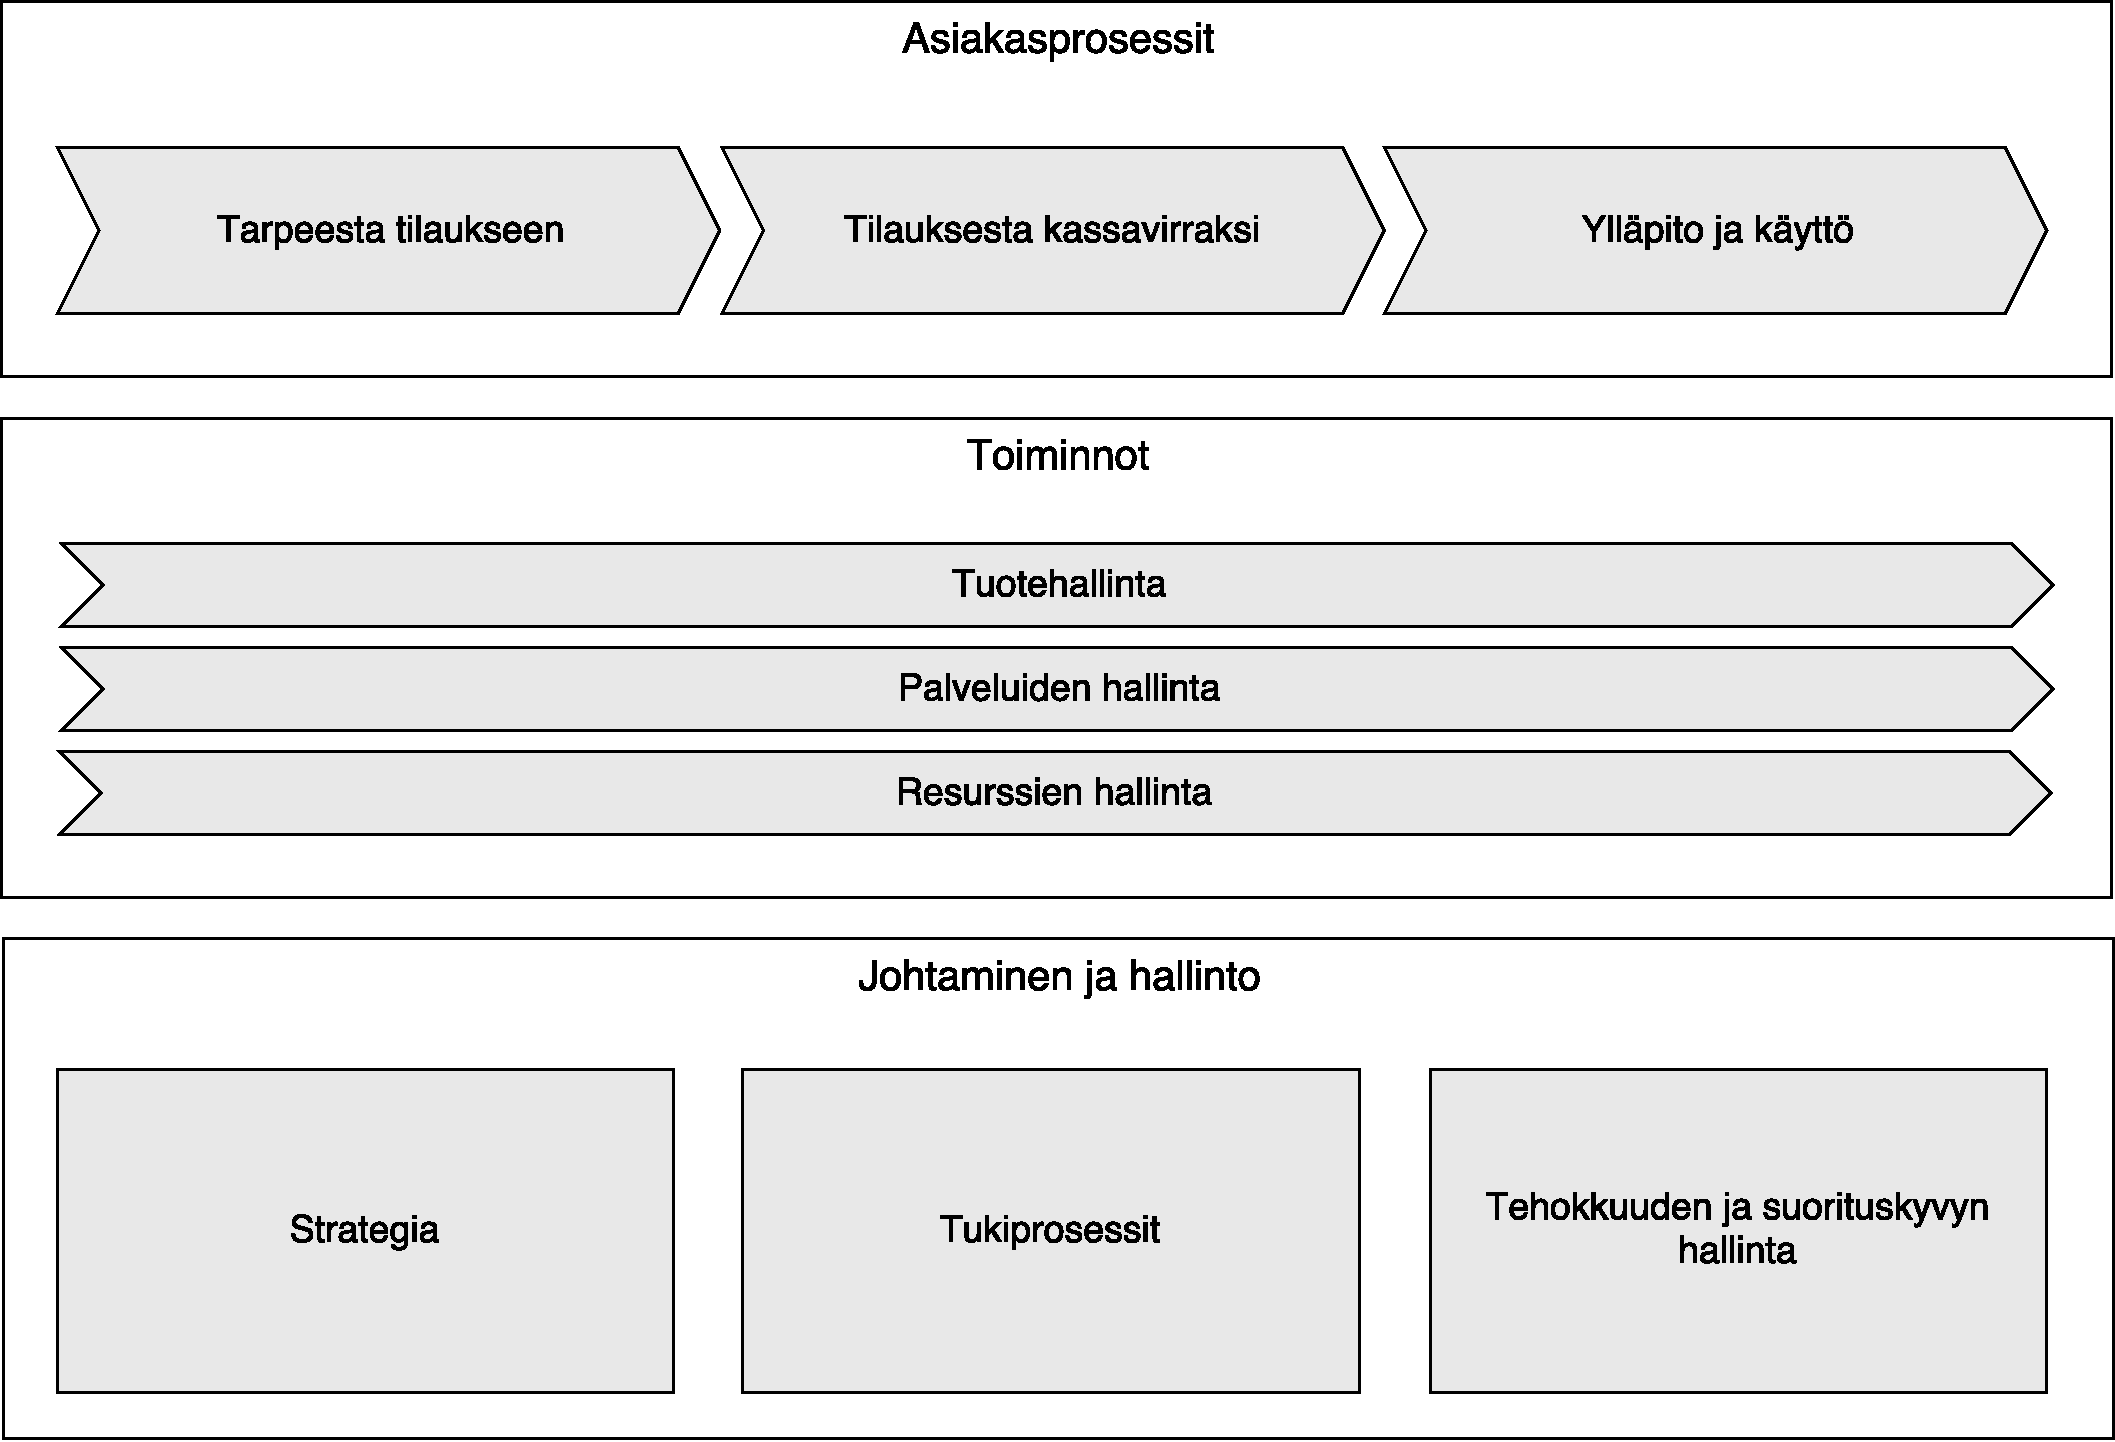
\includegraphics[scale=0.4]{images/prosessiarkkitehtuuri.pdf}
    \caption{Telian arvotuotannon prosessiarkkitehtuuri.}
    \label{fig:prosark}
\end{figure}

Siiloutunutta organisaatiomallia alettiin uusimaan prosessijohtamiseen perustuen. Segmentti ja tuotekohtaisia toimintamalleja alettiin muuttamaan perustumaan arvoketjujen ja elinkaarien johtamiseen koko liiketoiminnan kattavalla prosessimallilla. Tämän työn tuloksena määriteltiin uusi prosessiarkkitehtuuri, joka on kuvattuna kuvassa \ref{fig:prosark}. Jatkossa uusi prosessiarkkitehtuuri ja vanha toiminnallinen organisaatiomalli toimivat päällekäin, mutta toimintaa seurataan tarkemmin prosessien avulla. Kuten 2. kappaleessa kerrottiin, prosessiarkkitehtuuri kuvaa tietyn osaprosessin tehtävän, sijainnin ja tavoitteen yrityksen kokonaisarkkitehtuurissa. Se ei kuitenkaan anna vastausta siihen miten tämä käytännössä tehdään yrityksen IT-arkkitehtuurissa. Transformaatiohankeen vaikein osuus onkin juuri IT-järjestelmiin liittyvä osuus.\\

\textbf{IT-järjestelmäarkkitehtuurin muutos}\\

Analyysien mukaan kompleksisuutta tuovia ominaisuuksia on myös muissakin rakenteissa kuin organisaatiomallissa. Osin vanhasta organisaatiomallista ja vuosikymmeniä rakentuneesta IT-infrasta johtuen, IT-järjestelmien lukumäärä havaittiin korkeaksi, osin vanhanaikaiseksi, päällekäiseksi ja järjestelmät toimivat liiaksi toisista irrallaan. Toimintamallit ja käytetyt järjestelmät olivat erilaisia organisaation eri osissa. Esimerkiksi yritysasiakkaille tarjotuissa ratkaisuissa yksittäisten räätälöintien, hinnoittelumallien ja taustajärjestelmien määrän havaittiin tuovan turhaa kompleksisuutta, jota oli vaikea hallita. Laskutukseen ja asiakkuudenhallintaan käytettyjä järjestelmiä on myös useita, ja ne toimivat erillään. Jossain tapauksissa laskutus hoitui manuaalisesti Excel-työkalujen avulla. Tämän johdosta oli vaikea muodostaa kokonaisvaltaista näkymää asiakkaan ratkaisusta, ja useista erilaisista asiakkailla olevista laskutusmalleista. Myös kokonaisvaltainen näkymä asiakkailla käytössä olevista ja myytävissä olevista ratkaisuista oli vaikea muodostaa. Kokonaisuus järjestelmien osalta havaittiin kompleksiseksi ja vaikeasti hallittavaksi.\\

\begin{figure}[!h]
    \centering
    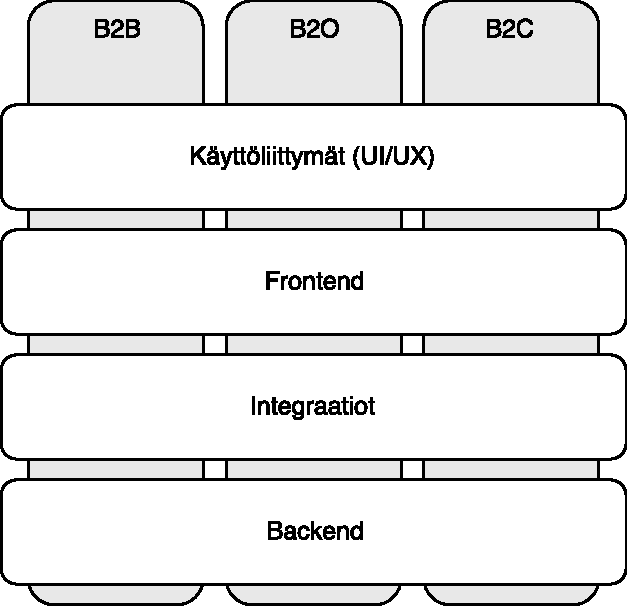
\includegraphics[scale=0.5]{images/ratkaisuarkkitehtuuri.pdf}
    \caption{Telian tavoitetilaa kuvaava IT-arkkitehtuuri.}
    \label{fig:ratkark}
\end{figure}

Transformaatiohanke lähti uudistamaan IT-järjestelmiä yllä mainittujen strategisten tavoitteiden pohjalta. Uudistustyön pohjana toimii IT-arkkitehtuurin tavoitetilan mukainen ratkaisuarkkitehtuuri, joka on esitettynä kuvassa \ref{fig:ratkark}. Tavoitearkkitehtuuri koostuu neljästä kerroksesta: Käyttöliittymä- ja frontend-kerroksista, joissa tavoitteena on parantaa asiakaskokemusta ja luoda uusia digitaalisia palveluita. Integraatio- ja backend-kerroksista, joissa tavoitteena on laskea kustannuksia ja kasvattaa laatua automaation ja migraatioiden avulla.\\

Käyttöliittymäkerros kuvaa kokoelmaa erilaisista kanavista, joista Telian asiakkaat käyttävät palveluitaan. Tämän kerroksen tarkoitus on antaa asiakkaille uusia parempia digitaalisia kanavia, joista Telian palveluita voi tilata ja hallinnoida. Aikaisemmin kuluttaja- ja yritysasiakkaille on ollut useita erilaisia järjestelmäratkaisuja ja toimintamalleja, joiden kautta palveluita hallitaan. Usein myös yksinkertaisissakin asioissa on ollut tarve kontaktoida Telian henkilöä palveluihin liittyvissä asioissa. Tämän kerroksen ratkaisujen avulla järjestelmien määrää halutaan pienentää ja suuri osa transaktioista halutaan siirtää uusiin digitaalisiin kanaviin. Tämän toivotaan parantavan asiakaskokemusta merkittävästi ja säästävän kustannuksia asiakaspalvelussa. Tämä kerros on vahvasti liitoksissa seuraavaan kerrokseen.\\

Frontend-kerros kuvaa näkymää asiakkaan palveluihin Telian henkilöille. Kuluttaja- ja yritysliiketoiminnassa ei aikaisemmin ole ollut tälläistä yhtenäistä näkymää, ja siksi sen rakentaminen koetaan tärkeäksi. Tälle kerrokselle on valittu yksi järjestelmä, joka käsittää tulevaisuudessa kaikki Telian kuluttaja- ja yritysasiakkaat. Tässä kerroksessa on myös helposti käytettävät näkymät erilaisiin asiakaspalvelutehtäviin ja myynnin työkalut. Tähän kerrokseen halutaan myös mallintaa kaikkia Telian tuotteet ja palvelut, koska tällä hetkellä tämä tieto on hajallaan erilaisissa järjestelmissä, erilaisina versioina tai se puuttuu kokonaan. Tämän kerroksen ratkaisujen avulla erilaisia tuotteita ja palveluita voidaan tuoda markkinoille nopeammin ja asiakkuuksia voidaan hallita tuloksekkaammin. Nämä kaksi ylempää kerrosta eivät kuitenkaan voi toimia ilman integraatiota taustajärjestelmiin.\\

Integraatio-kerros kuvaa sitä miten kaksi ylempää kerrosta yhdistyvät alemman backend-kerroksen tuotantojärjestelmiin. Aikaisemmin integraatioita lukuisten järjestelmien välillä rakennettiin yksittäisesti, jolloin erilaisten integraatioiden hallitseminen oli työlästä ja niiden uudelleenkäyttö ei ollut mahdollista. Jatkossa integraatio-kerros on kokoelma määriteltyjä rajapintoja, jossa on avoimia rajapintoja ja standarditeknologioita. Kerroksen avulla kumppanit ja asiakkaat voivat myös integroitua lähemmäs Telian ekosysteemiä. \\

Backend-kerros kuvaa tuotantojärjestelmiä, joissa asiakkaiden tuotteet ja palvelut toimivat, ja myös esimerkiksi laskutusjärjestelmiä. Tässä kerroksessa on vuosien mittaan rakentunut vanhojen järjestelmien kokoelma, ja myös uudet rakenteilla olevat järjestelmät. Tässä kerroksessa on myös laaja kokoelma erilaisia uusia ja vanhoja teknologioita, jonka vuoksi niiden kehittäminen on hidasta ja kallista. Tähän kerroksessa kompleksisuutta tuo myös aikaisemmin tuotelinjoitttain rakennetut tuotantojärjestelmät. Jatkossa tässä kerroksessa tavoitteena on karsia päällekkäisiä järjestelmiä ja hankkiutua eroon mahdollisimman suuresta määrästä järjestelmiä. Tämän avulla halutaan laskea kustannuksia laadukkailla ja virheettömästi toimivilla taustajärjestelmillä. Esimerkiksi tavoitteena on käyttää yhtä laskutusjärjestelmää tulevaisuudessa.\\

Transformaatiohankkeen läpivieminen nykytilasta tavoitetilaan uuden prosessiarkkitehtuurin ja IT-arkkitehtuurin avulla on iso muutos. Siksi sen läpivientiä ohjaa liiketoiminnan tavoitteet, joiden perusteella on valittu painopisteet.\\

\textbf{Transformaatiohankkeen painopisteet}\\

Transformaatiohankkeen ensimmäiksi painopisteiksi valittiin alueet, joissa oli suurin liiketoiminnallinen tarve saada tuloksia aikaan. Todettiin, että painopiste on aluksi kahdessa asiassa: Uudet tuotteet ja palvelut rakennetaan tukemaan prosessiarkkitehtuuria ja IT-arkkitehtuuria. Prosessiarkkitehtuurin ja IT-arkkitehtuurin osalta painopiste on alueissa, joissa voidaan kehittää yritysliiketoiminnan asiakaskokemusta.\\

Uusien tuotteiden ja palveluiden osalta tämä tarkoitti sitä, että niiden tulee käyttää tavoitteen mukaista IT-arkkitehtuuria. Eli näiden tuotteiden tai palveluiden tuottamiseen tulee käyttää IT-järjestelmiä, jotka toimivat myös tulevaisuuden IT-arkkitehtuurissa. Lisäksi tuotantoprosessien tulisi olla automatisoitu mahdollisuuksien rajoissa. Tämän vuoksi Kontakti L:n asiakasprosessille on myös asetettu tavoite automatisoinnista.\\

Yritysliiketoiminnan asiakaskokemuksen kehittämisessä todettiin, että tähän voitaisiin vaikuttaa eniten keskittymällä prosessiarkkitehtuurin (kuva \ref{fig:prosark}) asiakasprosesseista tarpesta tilaukseen-prosessiin. Tässä prosessissa on niiden toimintojen ketju, joiden perusteella asiakas saadaan tilaamaan tuote tai palvelu. Havaittiin, että tähän prosessiin voidaan vaikuttaa eniten kuvassa \ref{fig:ratkark} esitetyn IT-arkkitehtuurin kahdessa ylimmässä kerroksessa, jossa asiakaspolkua tukevia työkaluja voidaan rakentaa asiakkaan ja liiketoiminnan käytettäväksi.\\

Käytännön työtä on tehty pilotointien avulla rajatuissa kompakteissa toiminnoissa. Havaittiin, että toimintamallit uusissa digitaalisissa kanavissa eroavat suuresti vanhasta. Myynti, markkinointi ja asiakaspalvelu ovat erilaisia jatkossa, jonka vuoksi vasta uusien toimintamallien rakentamisen jälkeen voidaan nähdä mitä kannattaa rakentaa tai automatisoida teknologian avulla.\\

Seuraavassa alaluvussa kerrotaan Telian viestintäratkaisujen tuoteportfoliosta, joka on Telian transformaatiohankkeen lisäksi toinen Kontakti L:n automatisointia ajava asiakokonaisuus.

%Operatiivisen mallin muutos. myynti ja markkinointi asiakaspalvelu jne erilaista uusissa digitaalisissa kanavissa. iso liikeotiminnan muutos. vasta sen jälkeen tiedetään tarkemmin miten asiat kannattaa konfiguroida ja automatisoida. Sen takia liiketoiminta johtaa tätä ja sen jälkeen teknologia ja kanavat toteuttaa sen. Käyttäjälähtöistä kehitystä. 

%Tavoitetilan mukaisen prosessiarkkitehtuurin osalta todettiin, että tämä tarkoitti tarpeesta tilaukseen- asiakasprosessiin kehittämistä uusilla digitaalisilla teknologioilla. Tavoitetilan IT-arkkitehtuurin osalta tämä tarkoitti keskittymistä kahteen ylempään kerrokseen, eli käyttöliittymä- ja frontend-kerrokseen. Tarkoituksena oli siis tarjota puuttuva asiakashallinnan näkymä liiketoiminnalle, ja rakentaa asiakkaille paremmat työkalut käyttöliittymiin.\\

%Tämän jälkeen kokonaisuutta rajattiin koskemaan segmenttiä, jossa oli eniten liiketoiminnallista tarvetta parantaa asiakaskokemusta, ja missä saataisiin lyhyellä aikavälillä eniten liiketoiminnan tulosta aikaan (kuva \ref{fig:digivisio}). Eli kompakti ryhmä, jossa oli toistettavat toimintamallit ja voluumia asiakashallinnoinnissa.\\

%Ensimmäisissä piloteissa huomattiin, että uudet digitaaliset kanavat ja työkalut vaativat myös operatiivista muutosta. Olikin järkevä 

%Vanhojen toimintamallit ryhmätasolla esimerkiksi myynnissä ja markkinoinnissa eivät soveltuneet käytettäviksi uusien työkalu

%Transformaatiohankkeen painopisteet ovat olleet siellä missä lyhyellä aikavälillä voidaan saada eniten liiketoiminnallisia tuloksia aikaan, kuten 4. kappaleessa tuotiin esiin. Panopisteiksi valittiin tällä perusteella yritysliiketoiminnan keskisuuren asiakassegmentin asiakaspolun parantaminen ja uudet yrityksille lanseerattavat palvelut ja tuotteet.\\ 

%Tämä tarkoitti sitä, että prosessiarkkitehtuurin (kuva \ref{fig:prosark}) asiakasprosessin alkupää, tarpeesta tilaukseen -vaihe toimii keihäänkärkenä. IT-arkkitehtuurissa korostui sen vuoksi kaksi päällimäistä kerrosta, käyttöliittymä- ja frontend-kerros.

%Käytännössä tämä on tarkoittanut segmentin asiakkaille näkyvien asiakaskanavien käyttöliittymien uudistamisia ja segmenttiä palvelevien myyjien ja asiakaspalvelijoiden asiakasnäkymän rakentamista. 

%ei tavoittele kaikkien muutoksien läpivientiä kerralla, vaan 
%Transformaatiohankkeessa on paljon sisältöä ja tavoitteita, joten 

%otetaan käyttöön siellä missä lyhyellä aikavälillä voidaan saada eniten aikaan. Tämän vuoksi painopisteenä ovatkin olleet 
%Offer market ja sell
%asiakas se kenelle me näitä asioita teemme.
%B2B:ssä kipukohtia johon lähdettiin vaikuttamaan front endin kautta.
%Mikä on se mistä lähdetään liikkeelle?

%kaikki uudet tuotteet tuodaan target järjestelmiin. 

%Pienemmässä päässä nps haasteita ja noealla aikavälillä muutosta saada, kompaktin kokoinen ryhmä. heidän kanssa huomattavast ihelpompi harjoitella uuden homman rakentamista. Myös se että se on keskivaiheilla B2B tarjoomassa, jolloin onnistumiset voidaan hyödyntää ylhäällä ja alhaalla. 

%Mikä on se vaikein ja ensimmäinen ongelma? Asiakaskokemus se on. Puuttuvat työkalut crm ja muut liiketoiminnalle. Se mikä näkyy markkinalle. se mikä näkyy liikeotiminnalle ja antaa edellytykse t tehdä rahaa talolle.

%Operatiivisen mallin muutos. myynti ja markkinointi asiakaspalvelu jne erilaista uusissa digitaalisissa kanavissa. iso liikeotiminnan muutos. vasta sen jälkeen tiedetään tarkemmin miten asiat kannattaa konfiguroida ja automatisoida. Sen takia liiketoiminta johtaa tätä ja sen jälkeen teknologia ja kanavat toteuttaa sen. Käyttäjälähtöistä kehitystä. 

%\section{Case Kontakti L-tuotteen asiakasprosessi}

%Tässä kappaleessa käydään läpi Kontakti L:n asiakasprosessin nykytila. Nykytilan taustaksi kerrotaan Kontakti L:n liiketoimintatapaus, josta selviää asiakasprosessille asetetut vaatimukset. Tämän jälkeen käydään läpi itse asiakasprosessin nykytila kuvaamalla prosessin työvaiheet, näiden työvaiheiden kulku, prosessissa toimivat sidosryhmät ja käytetyt järjestelmät. Lopuksi kerrotaan haastatteluissa esiin nousseita haasteita asiakasprosessin nykytilassa.

\subsection{Kontakti L viestintäratkaisujen tuoteportfoliossa}

Kontakti L-tuote on uusi tuote Telian yrityksille suunnattujen viestintäratkaisujen tuoteportfoliota, jossa Kontakti L:n rooli on olla nopeasti toimitettava ja tarjota perusratkaisun lisäksi laajat integrointimahdollisuudet muihin alustoihin. Käydään seuraavassa läpi Kontakti L:n rooli tuoteportfoliossa kahdesta näkökulmasta, eli asiakassegmentin ja integroitavuuden osalta.\\

\textbf{Kontakti L:n asiakassegmentti}\\

Telian viestintäratkaisujen tuoteportfolio on jaettu asiakaspalvelujärjestelmien osalta kolmeen asiakassegmenttiin: Pieneen, keskikokoiseen ja isoon segmenttiin. Asiakassegmentit kuvastavat asiakaspalveluratkaisun toiminnallisuuden ja kompleksisuuden määrää, ei itse ratkaisua käyttävän asiakasyrityksen kokoa tai ratkaisun käyttäjämäärää. Kompleksisuudella viitataan erilaisten asiakaskohtaisten toiminnallisuuksien ja hinnoittelumallien rakentamiseen. Tuoteportfolio ja asiakassegmentit on esitetty kuvassa \ref{fig:segmentit}. Kontakti L-tuote sijoitetaan tuoteportfoliossa keskikokoiseen segmenttiin.\\

Kontakti L eroaa muista tuoteportfolion asiakaspalvelujärjestelmistä, koska se perustuu täysin Telian ulkopuolisen alihankkijan järjestelmään. Muut asiakaspalvelujärjestelmät ovat Telia-konsernin yhtiöissä kehitettyjä järjestelmiä.\\ 
\begin{figure}[!h]
    \centering
    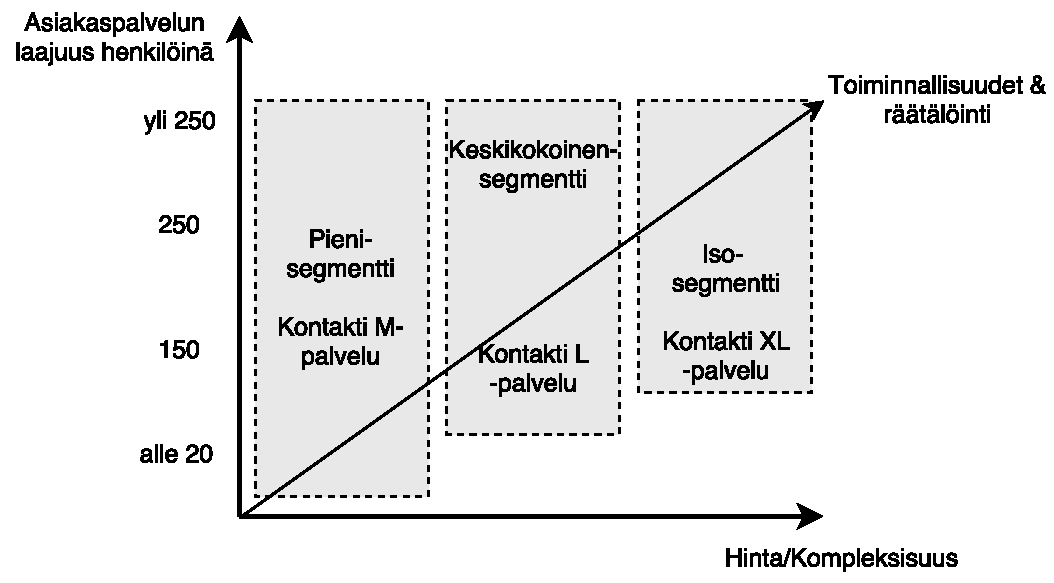
\includegraphics[scale=0.5]{images/segmentit.pdf}
    \caption{Telian asiakaspalvelujärjestelmien tuoteportfolio ja asiakassegmentit.}
    \label{fig:segmentit}
\end{figure}

Kuvan \ref{fig:segmentit} y-akseli esittää Telian asiakkaan asiakaspalvelussa työskentelevien henkilöiden lukumäärää. X-akseli taas esittää ratkaisun hintaa ja kompleksisuutta. Y- ja x-akseleiden välissä oleva nuoli kuvaa toiminnallisuuksien määrän kasvua ja myös eri räätälöintivaihtoehtojen lukumäärän kasvua. Kuvan laatikoilla esitetään miten tarpeeseen kukin ratkaisu soveltuu.\\

Asiakaspalvelujärjestelmien osalta Telia on ollut perinteinen toimija isossa segmentissä Kontakti XL-tuotteella, joka on ollut käytössä usean vuoden ajan. Sen tuottamisessa korostuu asiakaskohtaiset räätälöidyt toiminnallisuudet ja hinnoittelumallit. Myös toimitusajat ovat tällöin usein pitkiä ja ratkaisu toimitetaan asiakasprojektina. Tässä segmentissä Telia on ollut vahvin, kun taas keskikokoisessa ja pienessä segmentissä markkinaosuus on ollut heikko. Viime vuosina markkinassa onkin nähty kasvupotentiaalia nimenomaan keskikokoisessa ja pienessä segmentissä, jonka vuoksi tuoteportfoliota on täydennetty Kontakti M- ja Kontakti L-tuotteilla.\\

Pieneen asiakassegmenttiin kohdennettu Kontakti M-tuote on toiminnallisuuksilla ja räätälöintivaihtoehdoilla mitattuna yksinkertaisin ratkaisu asiakaspalveluun. Sen vahvuus on lähes automatisoitu toimitus ja asiakas voi tilata ja konfiguroida sen itse. Heikkoutena ratkaisussa on rajatut toiminnallisuudet ja integroitavuus muihin asiakkaan järjestelmiin. Tämän vuoksi Kontakti XL-tuotteen ja Kontakti M-tuotteen välille jäi tyhjiö.\\

Kontakti L-tuotteen tavoite onkin yhdistää Kontakti M- ja Kontakti XL-tuotteen parhaat puolet, eli sen tulisi olla nopeasti toimitettavissa, laskutettavissa ja tarjota perusratkaisun ohella hyvät mahdollisuudet eri alustoihin integroitumisessa, josta seuraavassa lisää.\\

\textbf{Kontakti L:n integroitavuus}\\

Kuten 3-kappaleessa tuotiin esiin, asiakaspalvelujärjestelmä integroituu yrityksen muihin järjestelmiin, kuten puheliikennettä hoitavaan järjestelmään, kalenteri- ja tilatiedon järjestelmiin sekä asiakashallinnan järjestelmiin. Markkinoilla on erilaisia alustoja joihin asiakaspalvelujärjestelmä integroituu näiden osalta, joista Telia tarjoaa pääasiassa kolmea vaihtoehtoa, jotka on esitetty kuvassa \ref{fig:palvelumal}.\\

\begin{figure}[!h]
    \centering
    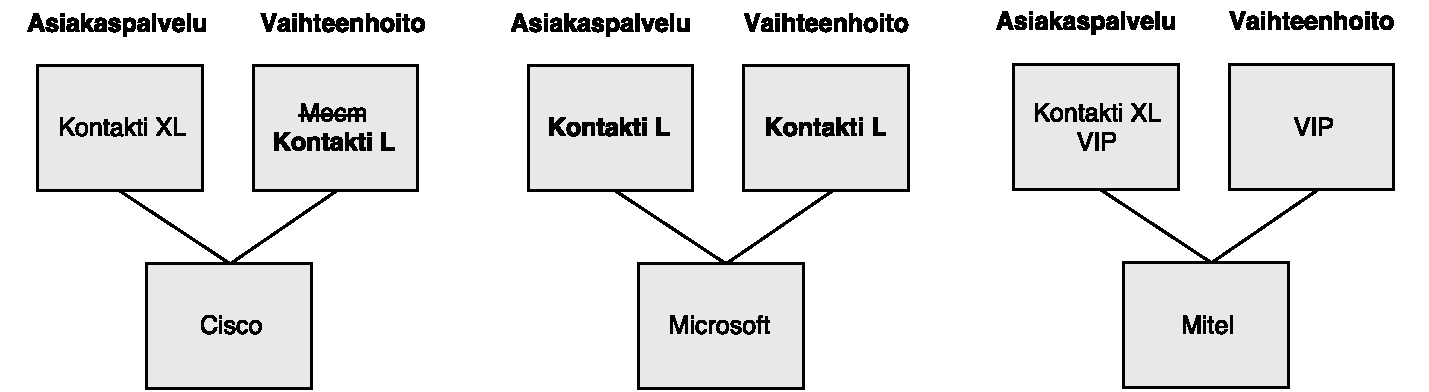
\includegraphics[scale=0.5]{images/palvelumalli.pdf}
    \caption{Telian asiakaspalveluratkaisun integroitavuus eri alustoihin.}
    \label{fig:palvelumal}
\end{figure}

%\begin{table}[]
%\centering
%\caption{My caption}
%\label{my-label}
%\begin{tabular}{|l|l|l|}
%\hline

%\textbf{Alusta:}    & \textbf{Asiakaspalvelujärjestelmä:} & \textbf{Vaihteenhoitojärjestelmä:}      \\ %\hline
%Cisco     & Kontakti XL               & Vanha: Mecm/ Uusi: Kontakti L \\ \hline
%Microsoft & Uusi: Kontakti L          & Uusi: Kontakti L              \\ \hline
%Mitel     & Kontakti XL/ VIP          & VIP                           \\ \hline
%\end{tabular}
%\end{table}

Kuvassa on esitettynä kolme eri alustaa ja kaksi erilaista ratkaisua asiakaspalvelujärjestelmän osalta. Asiakaspalvelujärjestelmä voi toimia joko perinteisenä asiakaspalvelussa käytettynä järjestelmänä tai vaihteenhoidon järjestelmänä. Kontakti L-tuotteen vahvuus onkin, että se voi toimia kumpanakin.\\

Kontakti L-tuotteella haettiin ratkaisua joka on integroitavissa Microsoftin alustan eri palveluihin. Aikaisemmin tuoteportfoliossa ei ollut ratkaisua jossa tämä onnistuisi täysin. Kontakti L-tuote myös korvaa tuoteportfoliossa elinkaarensa päässä olevan Mecm-tuotteen Ciscon ympäristössä.\\

\subsection{Kappaleen yhteenveto}

Tässä kappaleessa käytiin läpi miksi Kontakti L:n asiakasprosessi halutaan automatisoida. Automaatiota ajaa Telialla käynnissä oleva digitaalinen transformaatio ja viestintäratkaisujen tuoteportfolion tarve nopeasti toimitettavalle ratkaisulle, jossa on perusratkaisun lisäksi mahdollisuuksia integroitua muihin asiakkaan järjestelmiin.\\

Telian digitaalinen transformaatio ajaa automaatiota Kontakti L:n asiakasprosessiin, koska yksi sen painopiste on uusien tuotteiden ja palveluiden rakentaminen tavoitteen mukaiseen prosessi- ja IT-arkkitehtuuriin. Näin Kontakti L on osa kokonaisuutta joka on täyttämässä Telian strategiaa kilpailukykyisemmistä toiminnoista, joilta halutaan ketteryyttä ja kustannustehokkuutta uudella digitaalisella aikakaudella.\\

Telian viestintäratkaisujen tuoteportfoliossa asiakaspalvelujärjestelmien osalta Kontakti L:n asiakasprosessin automatisointia ajaa sen rooli keskisegmentissä, jossa yhdistyy ison ja pienen segmentin parhaat puolet. Keskisegmentin ratkaisun on oltava nopeasti toimitettavissa, mutta silti tarjota mahdollisuudet perusratkaisun lisäksi erilaisiin asiakaskohtaisiin integrointeihin. Nopeus ja asiakaskohtaiset integroinnit ovat kuitenkin ristiriidassa, ja tässä ristiriidan selvittämisessä automaatiolla on tärkeä rooli. Myös tavoitteena siirtää asiakasprosessissa tehtävää konfiguroitia asiakkaan tekemäksi itsepalveluksi.

Kontakti L:n asiakasprosessin tavoitteet vaativatkin uutta toimintamallia ja uusien teknologioiden hyödyntämistä. On tunnistettava perusratkaisu, joka voidaan automatisoida ja siirtää laskutukseen nopeasti tilauksesta, sekä tehdä vaatimuksien mukaiset integraatiot mahdolliseksi. On myös löydettävä ne toiminnot, jotka on järkevä siirtää itsepalveluun. Itsepalveluun tarvitaan myös käyttöliittymä, jonka kautta tehtävät toiminnot ovat helppoja asiakkaalle.\\

On myös ilmeistä, että näiden kahden asiakasprosessin automatisointia ajavien asiakokonaisuuksien taustalla on sama ilmiö. Uusia digitaalisia teknologioita ja ketteriä toimintamalleja hyödyntävät yritykset pystyvät luomaan uusia tehokkaampia tapoja ratkaista asiakkaan ongelma. Tällä on vaikutusta koko operaattorin liiketoimintaan ja nämä vaikutukset ovat nähtävissä myös yrityksille tarjottavien viestintäratkaisujen markkinoilla. \\

Seuraavassa kappaleessa pureudutaan Kontakti L:n asiakasprosessin nykytilaan, että voidaan arvioida sitä suhteessa sille asetettuihin tavoitteisiin.

%Kontakti L-tuote siis täydentää Telian viestintäratkaisujen tuoteportfoliota kahdella tavalla. Se tarjoaa ratkaisun asiakaspalvelujärjestelmien tuoteportfoliossa olleeseen aukkoon keskikokoisessa asiakassegmentissä, ja se tukee integraatiotioita Microsoftin alustan eri tuotteisiin.\\

%Telian kannalta markkinassa on eniten kasvupotentiaalia pienessä ja keskisuuressa asiakassegmentissä, jossa Telian markkinaosuus on pienin. Kappaleessa 4. mainittiin, että yrityksellä on kolme pääasiallista tapaa kehittää liiketoimintavalmiuksia markkinoilla: Kehitä tuotetta tai palvelua tekemällä siitä arvokkaampia asiakkaalle. Tehosta sisäisiä prosesseja tuottaaksesi arvo pienemmilläkustannuksilla. Paranna asiakaspolkua helpottamalla asiakkaan arvon hankkimista. Kuvan \ref{fig:digivisio} mukaan tavoite Kontakti L-tuotteen osalta onkin saada liiketoiminnan tuloksia aikaan tehostamalla prosesseja.

%Erityisesti Kontakti L-tuotteen osalta markkinaosuuden kasvattaminen keskisuuressa asiakassegmentissä on kiinni siitä onnistutaanko sen tuottamisessa yhdistämään Kontakti M- ja Kontakti XL-tuotteiden hyvät puolet. \\

%Asiakasprosessilta vaaditaankin nopeutta ja kustannustehokkuutta. Haaste Telian kannalta tässä onkin oikean toimintamallin löytäminen asiakasprosessissa. Kontakti L on myös uusi tuote, jonka myötä sille asetettiin uuden strategian mukaisesti tavoite korkeasta automaatioasteesta. Johdon asiakasprosessille asettama tavoite on 80-prosentin automaatio. Asiakasprosessissa tulisikin ottaa siksi huomioon sen yhteensopivuus tavoiteltuun IT-arkkitehtuuriin.
% Vendor ja IMS
%kestää pitkään että laskutus saadaan käyntiin toimituksen venyessä



%Large-segmentiin kohdennettu Kontakti XL-palvelu pohjautuu järjestelmään joka on ollut Telialla pitkään käytössä. Se on tarkoitettu asiakastarpeeseen, jolloin vaaditaan paljon erilaisia toiminnallisuuksia ja räätälöintejä, jolloin myös kustannukset ovat korkeat. Ratkaisun toimittaminen ja konfigurointi vie tällöin aikaa ja ratkaisu toimitetaan asiakaskohtaisesti projektina. Tämän kaltaisissa ratkaisuissa Telialla on iso rooli myös ylläpitovaiheessa. Tämä ratkaisu oli pitkään niin sanottu päätuote, joka integroituu Ciscon puheympäristöön ja vain osittain Microsoftin puheympäristöön. Tällöin havaittiin, että markkinassa on tarvetta hieman yksinkertaisemmalle ratkaisulle, joka on hankintakustannuksiltaan pienempi, nopeampi ottaa käyttöön, integroituisi täysin Microsoftin puheympäristöön ja soveltuisi myös pienemmän yrityksen asiakaspalveluun. Tämä tyhjiö tuoteportfoliossa jaettiin kahteen segmenttiin, low end- ja mid-segmenttiin, joihin päätettiin tuoda uudet ratkaisut.\\

 %Kyseinen ratkaisu ei integroidu muihin puheympäristöihin, vaan se käyttää omaansa. Asiakkaan kannalta ratkaisun hyötynä on nopea käyttöönotto, kustannustehokkuus ja helppo konfigurointi, jonka asiakas tekee itse. Telian kannalta ratkaisun hyötynä on lähes kokonaan automatisoitu toimitus ja asiakkaan itsepalveluna tekemä ylläpito, jonka vuoksi se ei sido resursseja ja on siten kustannuksiltaan pieni tuottaa. Kontakti M-palvelu toimii Internetin yli web-pohjaisena pilvipalveluna.\\

%Mid-segmentin osalta ratkaisu oli tuoda Kontakti L-palvelu markkinoille. Se tavoite on olla toiminnallisuuksiltaan lähes Kontakti XL:n tasoa, mutta tarjoata modernin asiakaspalvelujärjestelmän vaatimat toiminnallisuudet asiakkaille halvemmalla hinnalla, ja nopeammalla toimitusajalla. Kontakti L:n liiketoimintatapaus perustuukin halvempaan hintaan, joka on saavutettavissa tehokkaammalla toimitusprosessilla, ja integroitavuudella Microsoftin tuotteisiin ja puheympäristöön.

\section{Kontakti L:n asiakasprosessin nykytila}

Tässä kappaleessa käydään läpi Kontakti L:n asiakasprosessin nykytila. Nykytilan kuvaamiseksi kappaleessa kerrotaan ensin Kontakti L:n ratkaisuksi valitusta järjestelmästä. Tämän jälkeen esitetään yleiskuva sen asiakasprosessin nykytilasta, ja lisäksi esitetään mukana olevat sidosryhmät ja järjestelmät. Seuraavaksi kappaleessa käydään läpi asiakasprosessin eri vaiheet yksityiskohtaisesti läpi, josta ilmenee vaiheissa toimivat sidosryhmät ja järjestelmät. Lopuksi kiteytetään haastatteluissa esille nousseita haasteita asiakasprosessin eri vaiheissa.


Kuvassa \ref{fig:prosark} on kuvattuna Telian prosessiarkkitehtuuri korkealta tasolta. 


Telian prosessiarkkitehtuurin mukaan asiakasprosessi on 
Ongelmia erityisesti order-to-cash prosesseissa.
%Alt+0151

\subsection{Kontakti L:n asiakasprosessin määrittäminen}

Telian prosessiarkkitehtuuri (kuva \ref{fig:prosark}) määritteli kolme erilaista asiakasprosessia: Tarpeesta tilaukseen, tilauksesta kassavirraksi ja ylläpidon ja käytön. Tämän työn tarkastelussa on 2. kappaleessa esitetty asiakasprosessi, joka on prosessiarkkitehtuurin tilauksesta kassavirraksi —asiakasprosessi. Tilauksesta kassavirraksi —asiakasprosessi luo toimintamallit tuotteen tilaamiseen, toimittamiseen ja laskuttamiseen. Telian IT-arkkitehtuurin (kuvassa \ref{fig:ratkark}) näkökulmasta prosessissa painottuu backend-kerros, jossa sijaitsee tuotanto- ja laskutusjärjestelmät.\\

Kuten edellisessä kappaleessa tuotiin esiin, Telian digitaalisen transformaation painopiste on prosessiarkkitehtuurin tarpeesta tilaukseen asiakasprosessissa ja siten IT-arkkitehtuurin kahdessa ylimmässä kerroksessa. Tästä huolimatta, koska Kontakti L on uusi tuote, on sen tilauksesta kassavirraksi asiakasprosessille annettu tavoitteeksi 80\% automaatioaste käyttämällä IT-arkkitehtuurin tavoitejärjestelmiä.\\

Telian laatujärjestelmä määrittää asiakasprosesseille niiden kehitystä kuvaavan valmiusasteen. Kontakti L:n asiakasprosessi on tämän työn kirjoittamisen hetkellä hyväksytty valmiina myyntiin —asteelle. Tässä vaiheessa on selvillä tuotteen hinnasto ja yksityiskohdat. Asiakasprosessin toimintamallit eivät ole tässä vaiheessa vielä täysin valmiina, mutta toimituksia voidaan tehdä. Kontakti L ei ole vielä saanut hyväksyntää seuraavalle asteelle, joka on valmiina toimitukseen—aste. Tässä vaiheessa tuote tai palvelu on valmiina toimitettavaksi tilauksen perusteella ja kaikki asiakasprosessin toimintamallit ovat selvillä.\\

Kontakti L:n asiakasprosessin nykytila on selvitetty lähes valmiiden toimintamallien ja ohjeistuksien, sekä prosessissa toimivien sidosryhmien haastatteluiden perusteella.

Prosessin kehitysvaihe jossa ollaan menossa. RTS ei RTD
Jotain prosessin rakennusvaiheesta.

\subsubsection{Yleiskuva ja sidosryhmät}

Kuvassa \ref{fig:paavaih} on kuvattuna Kontakti L:n asiakasprosessin vaiheet ja tuotekehitys asiakasprosessin osana. Käydään seuraavaksi asiakasprosessin päävaiheet ja toimijat läpi.

\begin{figure}[!h]
    \centering
    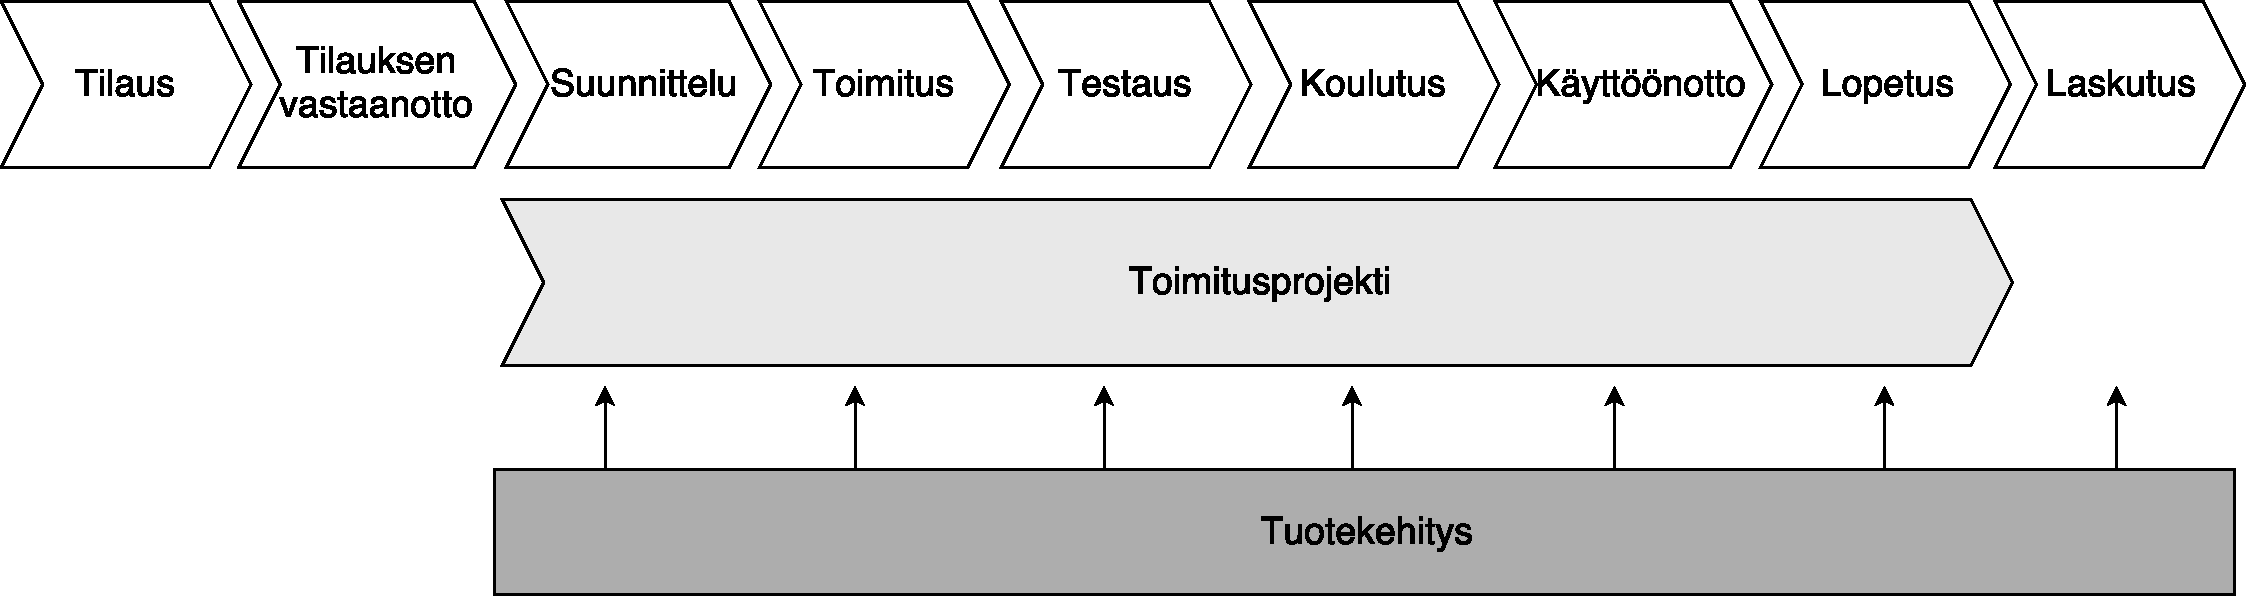
\includegraphics[scale=0.4]{images/ODI-prosessi.pdf}
    \caption{Kontakti L:n asiakasprosessin päävaiheet ja tuotekehitys.}
    \label{fig:paavaih}
\end{figure}

Kontakti L:n asiakasprosessi alkaa tilausvaiheesta. Tilausvaiheeseen tuleva syöte on tieto asiakkaan tarpeista. Vaiheen lopputulos on asiakashallinnan järjestelmään muodostuva tilaus asiakkaalle myydystä ratkaisusta, joka on syöte 



Kontakti L:n asiakasprosessi alkaa ratkaisun myyjän tekemästä tilauksesta, josta se välittyy tilauksen vastaanottoon. Tilauksen vastaanotossa toimii määrätyt henkilöt joiden tehtävä on varmistaa, että tilaus täyttää Kontakti L:n tilauksen minimivaatimukset. Tilauksen vastaanotto välittää minimivaatimukset täyttävän tilauksen Telian projektitoimiston työjonoon, josta alkaa suunnitteluvaihe.\\

Projektitoimiston esimies siirtää työjonosta tilauksen vastuutetulle projektipäällikölle. Projektipäällikön tehtävä on aloittaa toimitusprojekti ja valvoa projektin kulkua. Suunnitteluvaiheessa toimitusprojektin aloittamiseksi, projektipäällikön on käytävä tilaus läpi ja selvittää sen perusteella mitä resursseja toimitusprojekti tarvitsee. Projektipäällikön apuna toimitusprojektissa ovat toimitusvastaavat, jotka koordinoivat yksittäisten toimitettavien komponenttien toimitusta prosessissa.\\

Kun projektin vaatimat resurssit on hankittu, jatkuu suunnitteluvaihe puhe- ja IP-suunnittelijan tekemällä ratkaisun määrittelyllä. Määrittelyn tuloksena saadaan dokumentit, joiden avulla toimitusvaihe voi alkaa. Toimitusvaiheeseen päästään kun Kontakti L:n toimitusvastaava suorittaa ensin valmistelut toimitusta ja laskutusta varten. Toimitusvastaava tilaa projektipäällikön varamilta resursseilta toimituksen vaatimat työt, jolloin toimitusvaihe alkaa. Suunnittelu- ja toimitusvaihe tapahtuvat osin päällekäin.\\

Toimitusvaiheen alussa Tiedon työntekijä asentaa palvelimille vaaditut järjestelmän komponentit toimitusvastaavan tilauksesta ja käyttää suunnitteluvaiheessa luotuja määrittelydokumentteja. Kun asennus on kuitattu valmiiksi, toimitusvastaava tilaa järjestelmän konfigurointityön resurssivarauksen mukaiselta Telian järjestelmäasiantuntijalta, joka jälleen tekee vaadittavat konfiguroinnit ja integraatiot määrittelydokumenttien perusteella. Kun työ kuitataan valmiiksi alkaa ratkaisun testausvaihe.\\

Testausvaiheeseen ei ole toistaiseksi määritelty ohjeistusta, jonka mukaan testaus tulisi tehdä. Haastatteluiden perusteella testausta on kuitenkin tehnyt edellisen vaiheen järjestelmäasiantuntija ja puhesuunnittelija. Kun on todettu, että järjestelmä on toiminnassa alkaa koulutusvaihe.\\

Koulutusvaiheessa resurssivarauksen mukaisen kouluttajat aikatauluttavat ja suunnittelevat asiakkaalle tehtävät koulutukset toimitusvastaavan tilauksen perusteella. Kouluttajat opettavat asiakkaan käyttäjiä järjestelmän käytössä ja varmistavat, että käyttäjillä on tarvittavat kyvyt ja tukimateriaali kun järjestelmä otetaan käyttöön. Koulutusvaiheen jälkeen Kontakti L on valmiina käyttöönottoon. Koulutusvaihe ja käyttöönottovaihe tapahtuvat osin samanaikaisesti.\\

Käyttöönottovaiheessa projektipäällikkö ja toimitusvastaava sopivat aikataulun asiakkaan kanssa käyttöönoton ajasta. Aluksi asiakas tekee järjestelmän hyväksymistestauksen oman ohjeistuksensa mukaan. Telian järjestelmäasiantuntija tukee ohjeistuksen mukaan asiakasta käyttöönotossa. Kun asiakas on ottanut järjestelmän käyttöön, alkaa toimitusprojektin lopetusvaihe.\\

Lopetusvaiheessa projektipäällikkö käynnistää asiakkaan laskutuksen ja vapauttaa resurssivaraukset toimitusprojektilta. Viimeisessä laskutusvaiheessa tuotepäällikkö aloittaa Kontakti L:n kuukausilaskutuksen ja laskuttaa myös toimitusvaiheen työt asiakkaalta. Asiakasprosessi päättyy tähän.\\

Tuotekehitys on mukana asiakasprosessissa suunnitteluvaiheesta asti tukemalla muiden sidosryhmien työvaiheita ja koordinoimalla asiakasprosessissa esiin noussseita kehitystöitä alihankkijoilta.

 

- Asiakas
- Myyjä
- Tilausten vastaanottaja
- Projektitoimisto
- Projektipäällikkö
- Toimitusvastaava
- Tuotepäällikkö
- Tuotekehityspäällikkö
- Tieto L3
- Zylinc
- Tuotantopäälliköt
- Puhesuunnittelija
- IP-suunnittelija
- L2 konfiguroija
- Kouluttaja
- Tallentaja

Muut prosessit:
-RaVa-prosessi
-Datanet/SPVA-toimitusprosessi
-Mobiilitoimituksen prosessi
-Tuotekehitysprosessi
-Ylläpitoprosessi

Järjestelmät
- Tellu
- MultiBella
- Tiksu
\subsubsection{Prosessin läpikäynti}

Tässä osiossa käymme läpi Kontakti L:n asiakasprosessin kulun vaihe kerrallaan. Ensin käydään läpi yksittäisen vaiheen kulku, ja samalla kuvataan vaiheen riippuvuutta muihin prosessin vaiheisiin. Kuvauksessa tuodaan esiin vaiheen toimijat, dokumentit ja järjestelmät. Tämän osion tavoite on antaa tarkka kuva Kontakti L:n asiakasprosessin toiminnasta. Asiakasprosessin eri vaiheita kuvataan Telian niille käyttämillä termeillä.\\

\textbf{Tilausvaiheen kulku}\\

Vaiheen kesto on arvioitu olevan noin 1 päivä.\\

Kontakti L:n asiakasprosessi alkaa myyjän tekemästä tilauksesta, ja tämä vaihe on kuvattu kuvassa \ref{fig:tilaus}. Tätä ennen asiakas on hyväksynyt tarjouksen ja myyjä on varmistanut asiakaspalvelujärjestelmän toimitusajan erillisen varmennusprosessin kautta. Saatuaan päätöksen toimitusajasta, myyjä tekee palvelusopimuksen asiakkaan kanssa, jonka liitteeksi lisätään palvelutasosopimus, palvelun yksityiskohtaiset tiedot sisältävän palvelukuvauksen, palvelun hinnaston ja toimitusehdot.

\begin{figure}[!h]
    \centering
    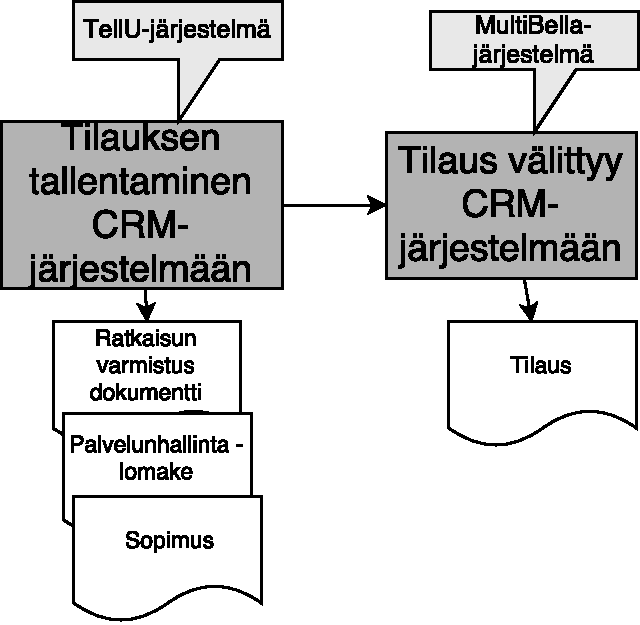
\includegraphics[scale=0.4]{images/tilausv.pdf}
    \caption{Kontakti L:n asiakasprosessin tilausvaihe.}
    \label{fig:tilaus}
\end{figure}

Kun sopimusosapuolet ovat allekirjoittaneet sopimuksen, myyjä tekee tilauksen Tellu-järjestelmän kautta, jossa tilaus tehdään lomakepohjaisen verkkosivun kautta. TellU-järjestelmä on Telian myynnin käytössä oleva asiakashallinnan järjestelmä. Tilauksen mukaan myyjä liittää varmennusprosessin tekemän päätöksen toimitusajasta, sopimuksen ja täytetyn palvelunhallintalomakkeen. Palvelunhallintalomake on Excel-tiedosto, jossa on valmis lomake-pohja myydyn asiakaspalvelujärjestelmän tietoja varten. Myyjän tehtyä tilauksen, välittyy se automaattisesti toiseen Telian käyttämään asiakashallinnan järjestelmään nimeltä MultiBella.\\

\textbf{Tilausten vastaanotto-vaiheen kulku}\\

Vaiheen kesto on arvioitu olevan noin 1 päivä.\\

Tilauksen vastaanotto-vaihe alkaa kun tilauksen vastaanotossa työskentelevä henkilö ottaa tilauksen käsittelyyn työjonostaan MultiBella-järjestelmässä. Henkilö tekee tilaukselle esitarkistuksen. Esitarkastuksen ensimmäisessä vaiheessa asiantuntija tarkastaa, että tilauksen mukana on hyväksytty päätös ratkaisun toimitusajasta. Toisessa vaiheessa hän tarkastaa, että tilauksesta löytyy minimivaatimukset.\\

\begin{figure}[!h]
    \centering
    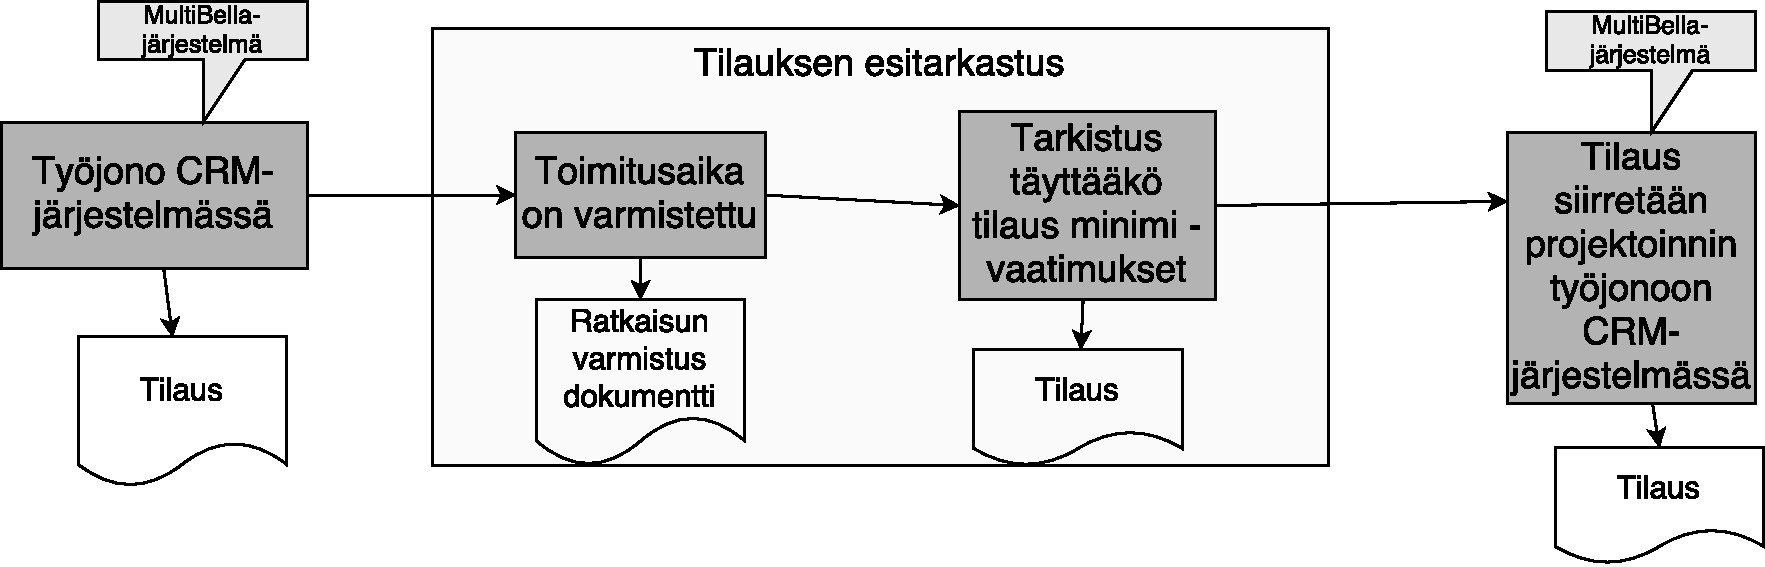
\includegraphics[scale=0.4]{images/tilvast.pdf}
    \caption{Kontakti L:n asiakasprosessin tilauksen vastaanotto-vaihe.}
    \label{fig:tilausvast}
\end{figure}

Minimivaatimukset täyttävä tilaus sisältää: palvelun lisenssien ennakoidut kappalemäärät, mahdolliset integraatioit muihin palveluihin ja sopimuksen yksikköhinnat. Asiantuntija siirtää minimivaatimukset täyttävän tilauksen projektitoimiston työjonoon MultiBella-järjestelmässä, jolloin tilauksen vastaanotto-vaihe päättyy\\

\textbf{Suunnitteluvaihe}\\

Vaiheen kesto on arvioitu olevan noin 1-2 kuukautta.\\

\begin{figure}[!h]
    \centering
    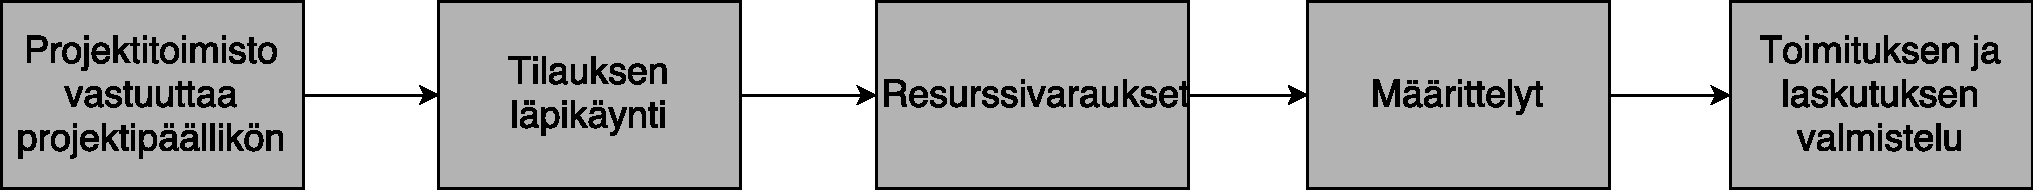
\includegraphics[scale=0.35]{images/ykssuunn.pdf}
    \caption{Kontakti L:n asiakasprosessin yksinkertaistettu suunnitteluvaihe.}
    \label{fig:ykssuun}
\end{figure}

Toimituksen suunnitteluvaihe käsittää asiakastoimituksen valmisteluun liittyvät työvaiheet: Toimitusprojektin aloitustoimet, jossa tilauksen sisältö tarkastetaan. Projektin resurssivaraukset, eli ihmiset, jotka tekevät seuraavat työvaiheet. Ratkaisuun liittyvän määrittelytyön. Viimeisenä toimituksen ja laskutuksen valmistelun. Tämän vaiheen tuloksena on projektisuunnitelma ja määrittelydokumentit. Käsitellään näitä neljää suunnitteluvaiheen osasta erillään.\\

\textbf{Suunnitteluvaihe: Tilauksen läpikäynti}\\

Suunnitteluvaiheen aloitustoimiin päästään kun projektitoimiston esimies on vastuuttanut projektipäällikön Kontakti L:n toimitusprojektille MultiBella-järjestelmän tilauksen perusteella. Kuvassa \ref{fig:aloitustoimet} on esitettynä tämä osuus suunnitteluvaiheesta. Projektipäällikkö käynnistää toimitusprojektin hankkimalla sille projektinumeron ProofX-järjestelmässä, johon kustannukset voidaan kohdentaa. Tämän jälkeen hän järjestää tapaamisen Kontakti L:n tuotepäällikön ja tuotekehityspäällikön kanssa tilauksen läpikäymiseksi. \\

\begin{figure}[!h]
    \centering
    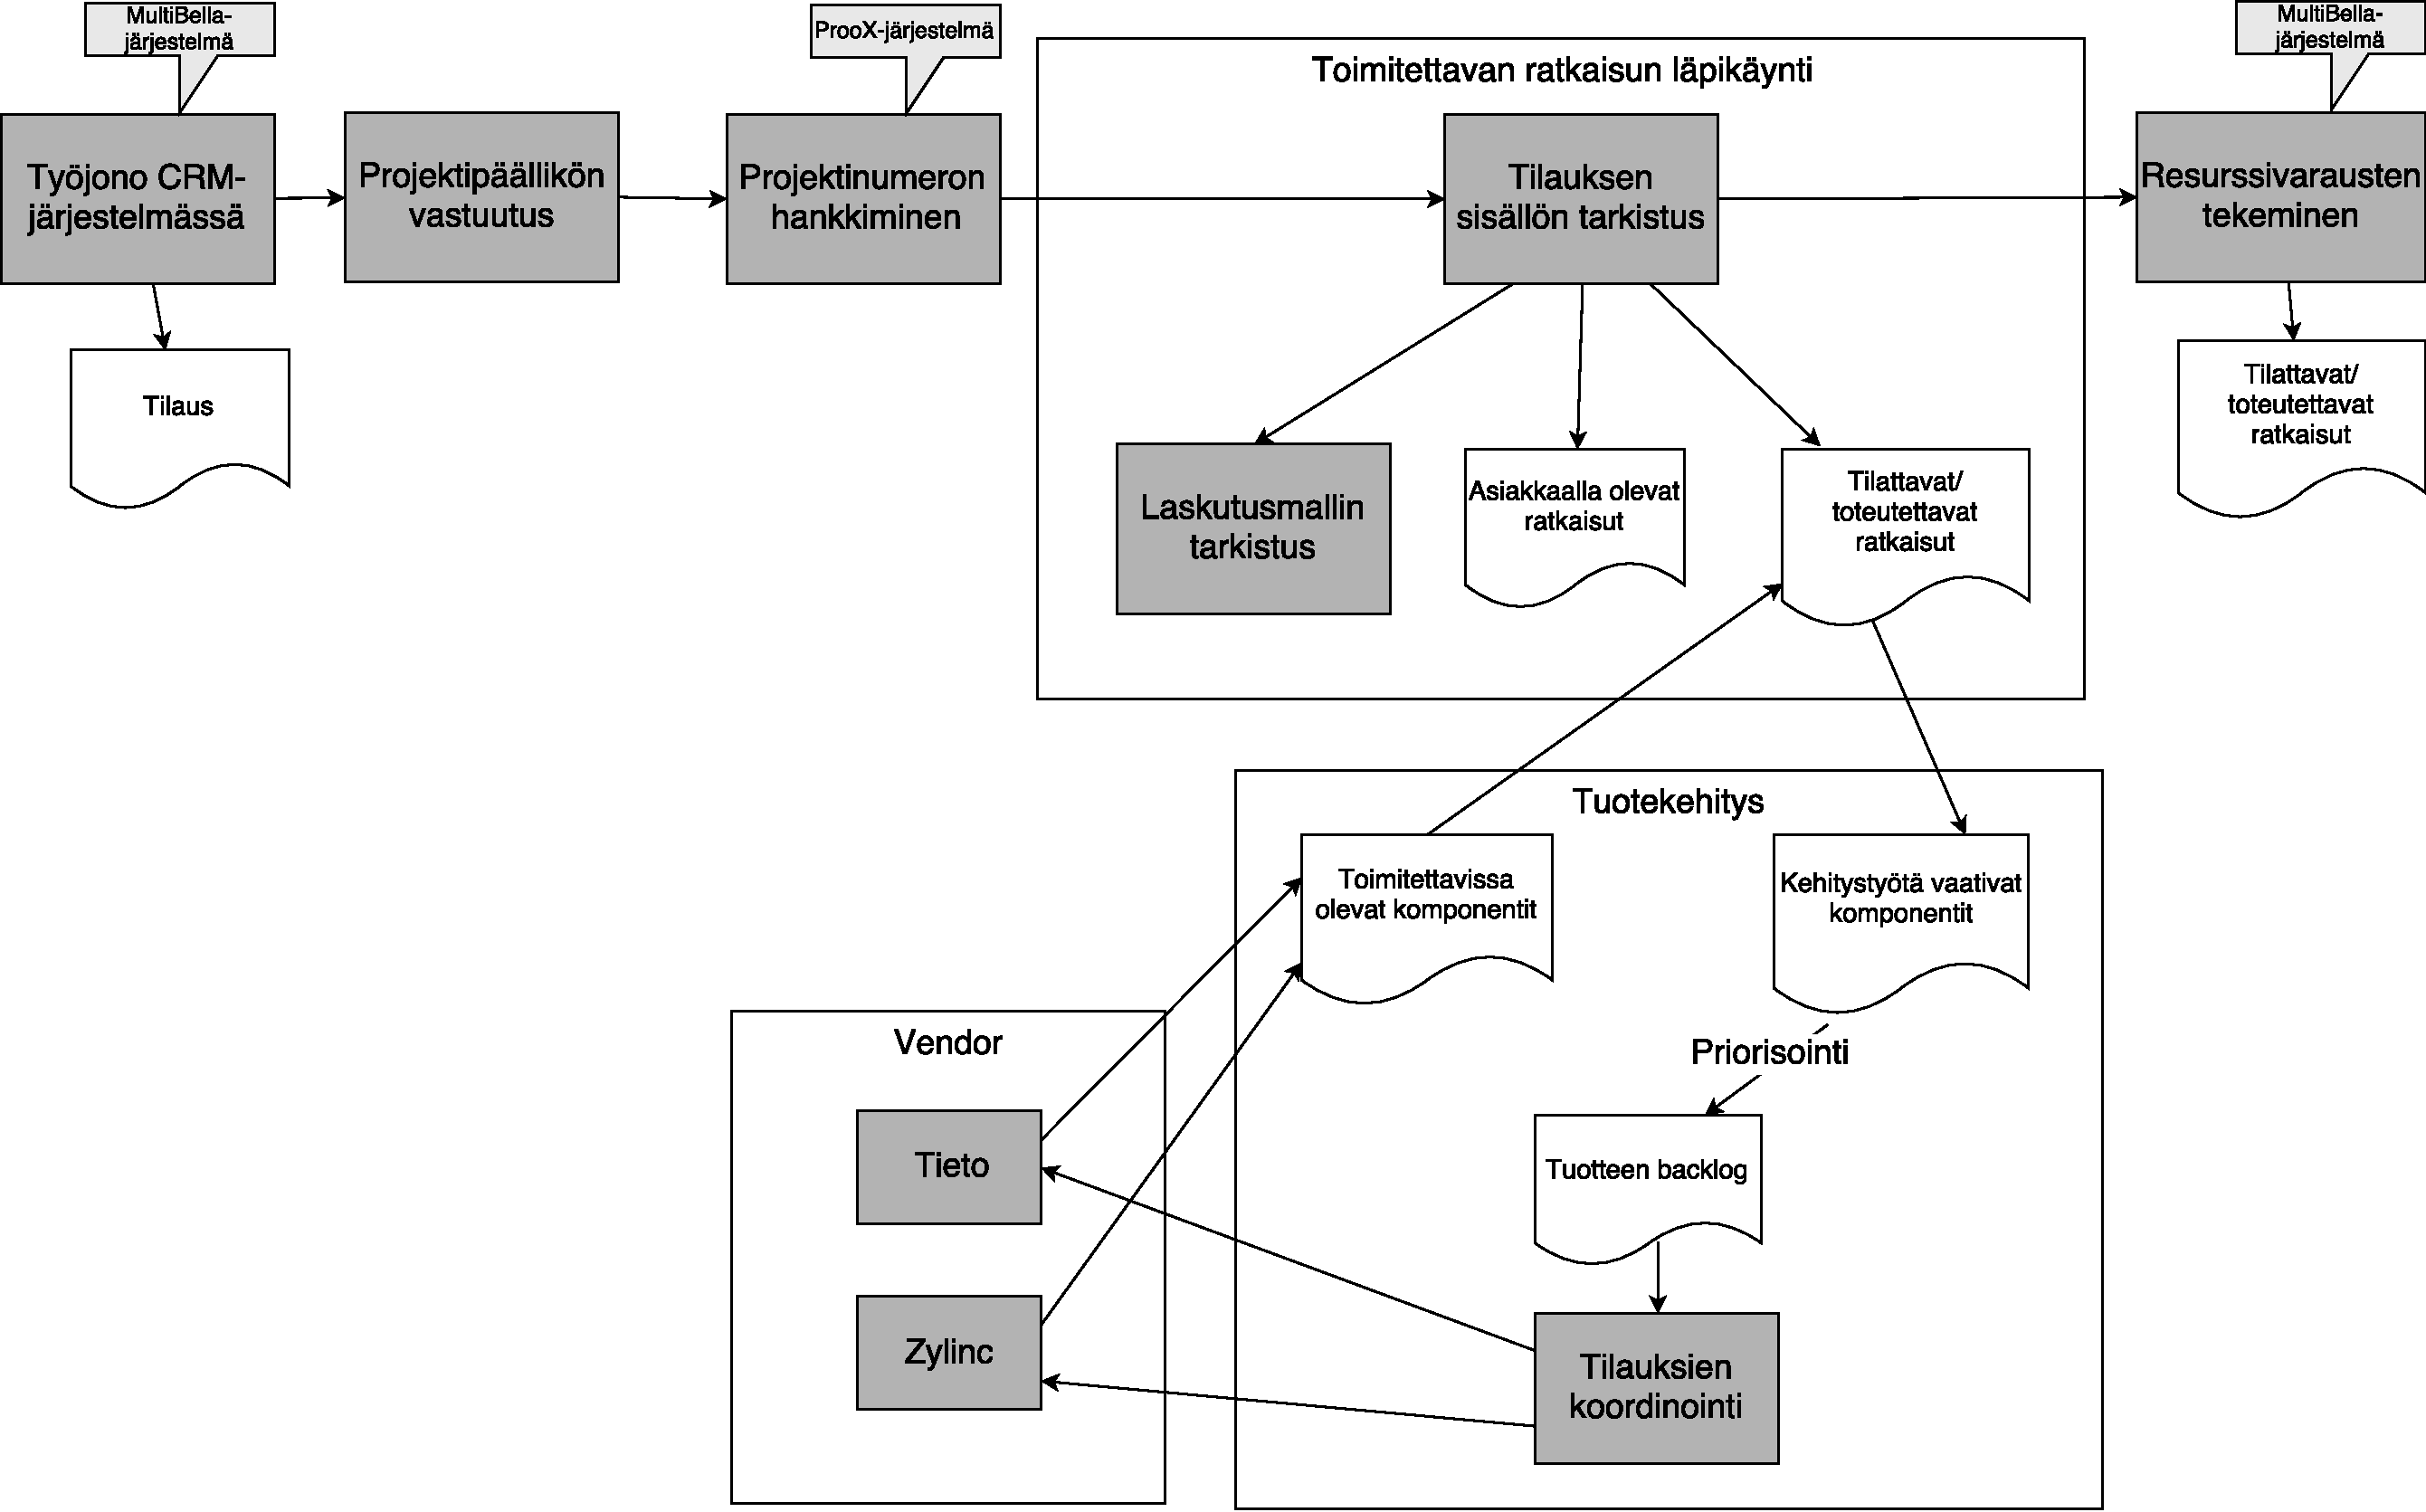
\includegraphics[scale=0.3]{images/aloitus.pdf}
    \caption{Kontakti L:n asiakasprosessin suunnitteluvaiheen tilauksen läpikäynti.}
    \label{fig:aloitustoimet}
\end{figure}

Tapaamisessa tilauksesta tarkistetaan minkälaista laskutusmallia asiakkaan kanssa tulisi käyttää, mitä viestintäratkaisuun kuuluvia komponentteja asiakkaalla jo on käytössä, ja mitä viestintäratkaisun komponentteja asiakkaalle tulee tilauksen perusteella toimittaa.\\

Kun toimitettavat komponentit ovat tunnistettu, jaetaan ne kahteen kategoriaan: Komponentteihin jotka on toimitettavissa ja kehitystyötä vaativiin komponentteihin. Toimitettavilla komponenteilla on resurssi, jolla on siihen liittyvä osaaminen ja ohjeistus. Kehitystyötä vaativat komponentit asetetaan tuotteen backlogiin priorisoidusti muiden siellä jo olevien komponenttien kanssa.\\

Kontakti L:n tuotepäällikkö ja tuotekehityspäällikkö priorisoivat backlogissa olevia komponentteja, ja tilaavat niihin liittyvän toteutuksen alihankkijalta. Se kumpaa alihankkijaa käytetään riippuu vaaditusta kehitystyöstä. Tieto tekee Telian palvelinalustaan liittyvät toimenpiteet ja Zylinc itse tuotteeseen liittyvän kehitystyön.\\

Kun toimitettavat komponentit on tunnistettu ja kehitystyötä vaativien komponenttien aikataulu on selvillä, tekee projektipäällikkö näiden komponenttien toimittamiseen liittyvät resurssivaraukset.\\

\textbf{Suunnitteluvaihe: Resurssivaraukset}\\

Toimitettavien komponenttien perusteella projektipäällikkö aloittaa resurssivarausten tekemisen. Kuvassa \ref{fig:resurssit} on esitettynä resurssivarausten osat. Ensimmäisenä projektipäällikkö tilaa Datanet-yhteyden asiakkaalle Tomaatti-järjestelmän kautta jos asiakkaalla ei vielä olemassaolevaa yhteyttä. Seuraavaksi hän tekee toimitusvastaavan resurssivarauksen MultiBella-järjestelmän kautta, ja sopii hänen kanssaan roolit toimitusprojektin ajaksi.\\

\begin{figure}[!h]
    \centering
    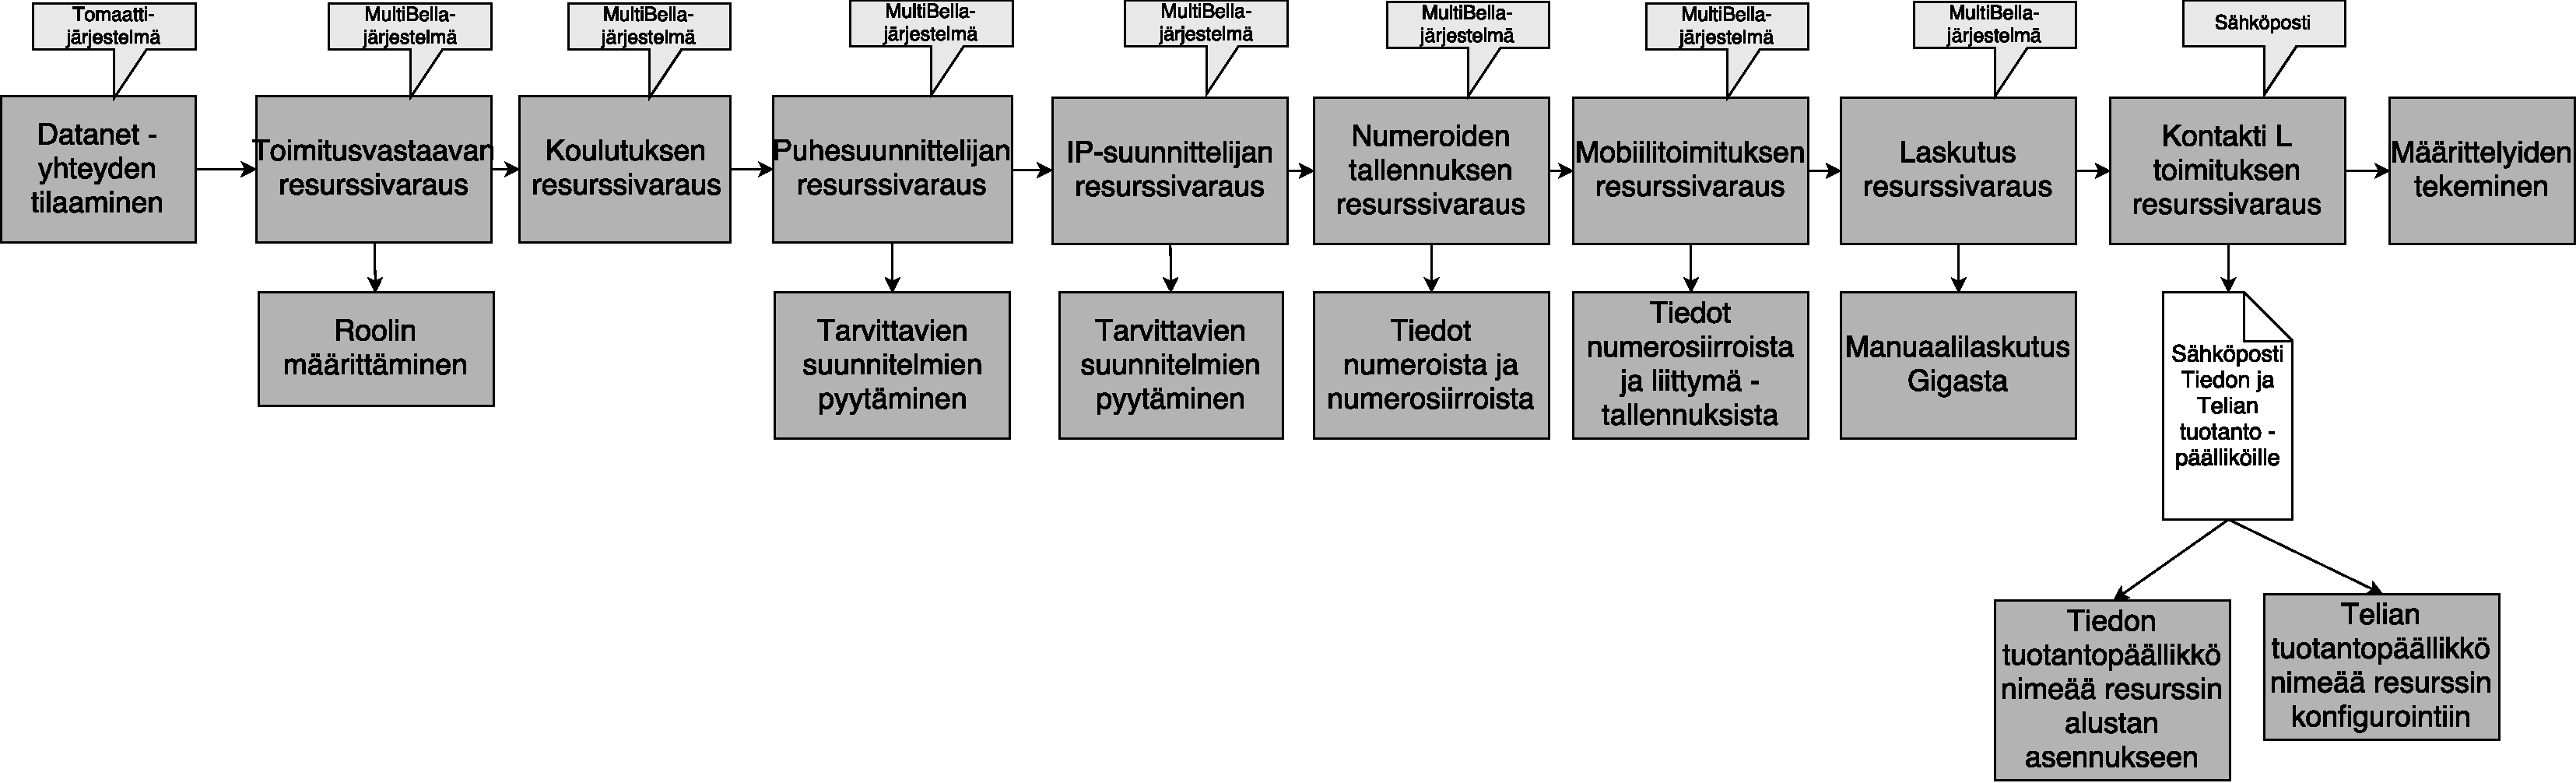
\includegraphics[scale=0.25]{images/resurssivaraukset.pdf}
    \caption{Kontakti L:n asiakasprosessin suunnitteluvaiheen resurssivaraukset.}
    \label{fig:resurssit}
\end{figure}

Tämän jälkeen projektipäällikkö tarkastaa sopimuksessa vaaditun koulutustarpeen, ja tekee sen perusteella resurssivarauksen MultiBella-järjestelmästä. Sen jälkeen hän varaa resurssin puhe- ja IP-suunnitteluun ja pyytää heiltä sopimuksessa mainitut suunnitelmat ratkaisun toimittamiseksi.\\

Seuraavaksi projektipäällikkö varaa resurssin palvelunumeroiden ja mobiilinumeroiden toimituksilta, ja välittää heille tiedot ratkaisussa käytetyistä numeroista, numerosiirroista ja uusien liittymien avaamisesta. Laskutuksen henkilöresurssin varaaminen on toistaiseksi epäselvää, ja sen vuoksi Kontakti L:n tuotepäällikön vastuulla. Toistaiseksi tuotepäällikkö on hoitanut laskutuksen itse manuaalisesti Giga-laskutusjärjestelmästä. Laskutuksen resurssia kuitenkin tarvitaan uuden yrityksen luomisessa, joten resurssi varataan silloin MultiBella-järjestelmästä joko tuotepäällikön tai projektipäällikön toimesta.\\

Viimeiseksi projektipäällikkö varaa resurssit järjestelmän asennukseen ja konfigurointiin lähettämällä sähköpostin Tiedon ja Telian järjestelmäasiantuntijoiden esimiehille eli tuotantopäälliköille. Tuotantopäälliköt nimeävät resurssit tehtäviinsä vastaamalla tähän sähköpostiin.\\

Kun kaikki resurssivaraukset on tehty, päästään aloittamaan ratkaisun määrittelytyö.\\

\textbf{Suunnitteluvaihe: Määrittelyt}\\

Kuvassa \ref{fig:maarittely} on esitettynä suunnitteluvaiheen määrittelyt. Ratkaisun määrittelytyö alkaa projektipäällikön järjestämässä tapaamisessa asiakkaan edustajien kanssa, jossa on mukana toimitusprosessissa olevat resurssit. Tapaamisen tarkoitus on tarkentaa tilauksen tietoja, sopia yhteisistä toimintamalleista, yhteyshenkilöistä ja aikataulusta. Tämän tapaamisen jälkeen projektipäällikkö järjestää vielä toisen tapaamisen sisäisesti toimitusorganisaation kanssa.\\

\begin{figure}[!h]
    \centering
    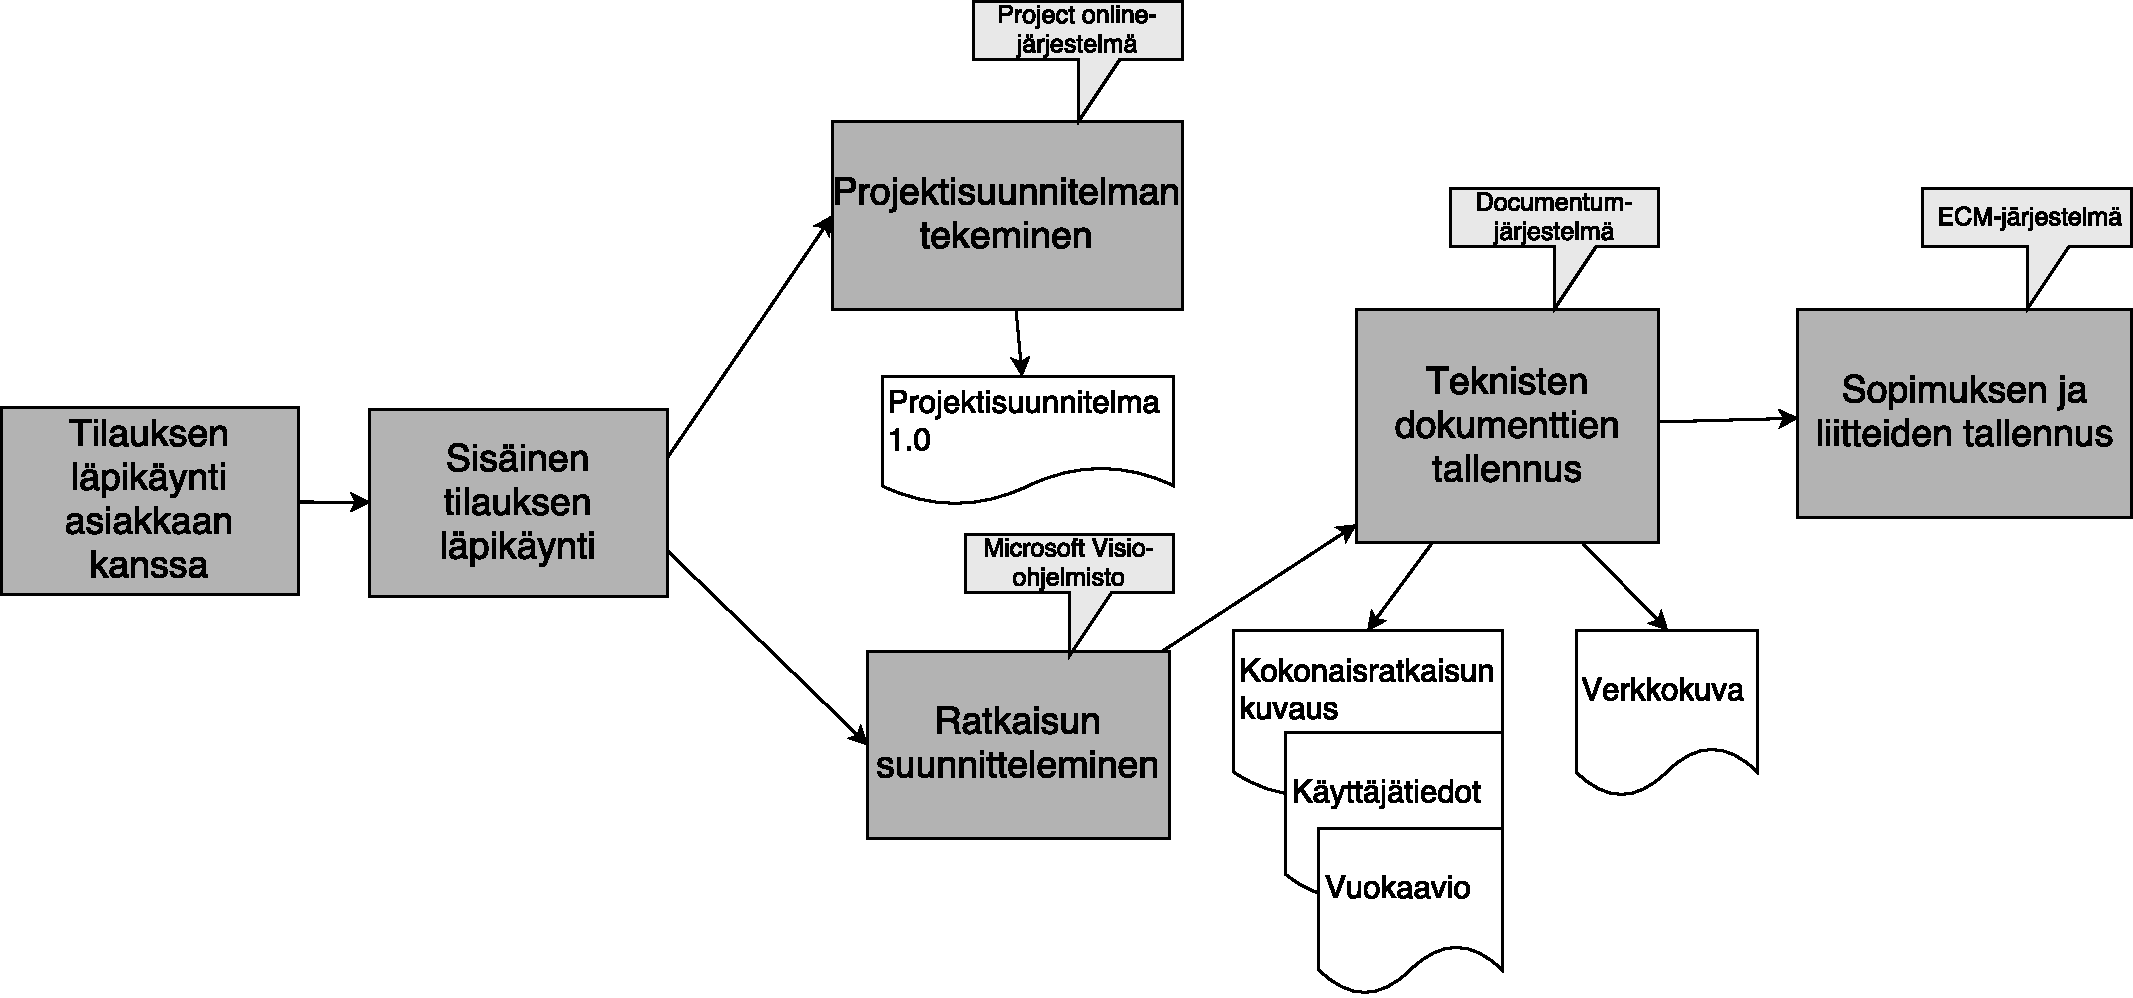
\includegraphics[scale=0.25]{images/maarittely.pdf}
    \caption{Kontakti L:n asiakasprosessin suunnitteluvaiheen määrittelyt.}
    \label{fig:maarittely}
\end{figure}

Kun yhteisistä toimintamalleista on sovittu, projektipäällikkä tekee projektisuunnitelman ensimmäisen version Project online projektisuunnittelujärjestelmässä. Samanaikaisesti puhesuunnittelija ja IP-suunnittelija aloittavat ratkaisun suunnittelun. He suunnittelevat ratkaisun yhteistyössä asiakkaan yhteyshenkilöiden kanssa. Suunnittelutyö dokumentoidaan Microsoft Visio-ohjelmalla. Puhesuunnittelijan työn tuloksena syntyy kuvaus kokonaisratkaisuista ja sen eri komponenteista ja vuokaavio ratkaisun numeroista, jonoista ja komponenteista. Puhesuunnittelija myös kerää asiakkaan käyttäjätiedot. IP-suunnittelijan työn tuloksena syntyy verkkokuva, josta ilmenee ratkaisun yhteydet, IP-osoitteet ja verkot. Suunnittelijat tallentavat dokumentit Documentum versiohallinnan järjestelmään.\\

Lopuksi toimitusvastaava vie sopimuksen liitteineen ECM-järjestelmään. Jo tämän vaiheen aikana toimitusvastaava on aloittanut toimituksen ja laskutuksen valmistelun.\\ 

\textbf{Suunnitteluvaihe: Toimituksen ja laskutuksen valmistelu}\\

Jo määrittelyiden tekemisen aikana toimitusvastaava aloittaa valmistelemaan toimitusta ja laskutusta. Kuvassa \ref{fig:valmtoimlask} on esitettynä tämän vaiheen kulku. Tämä vaihe on osittain päällekäinen toimitusvaiheen kanssa.

\begin{figure}[!h]
    \centering
    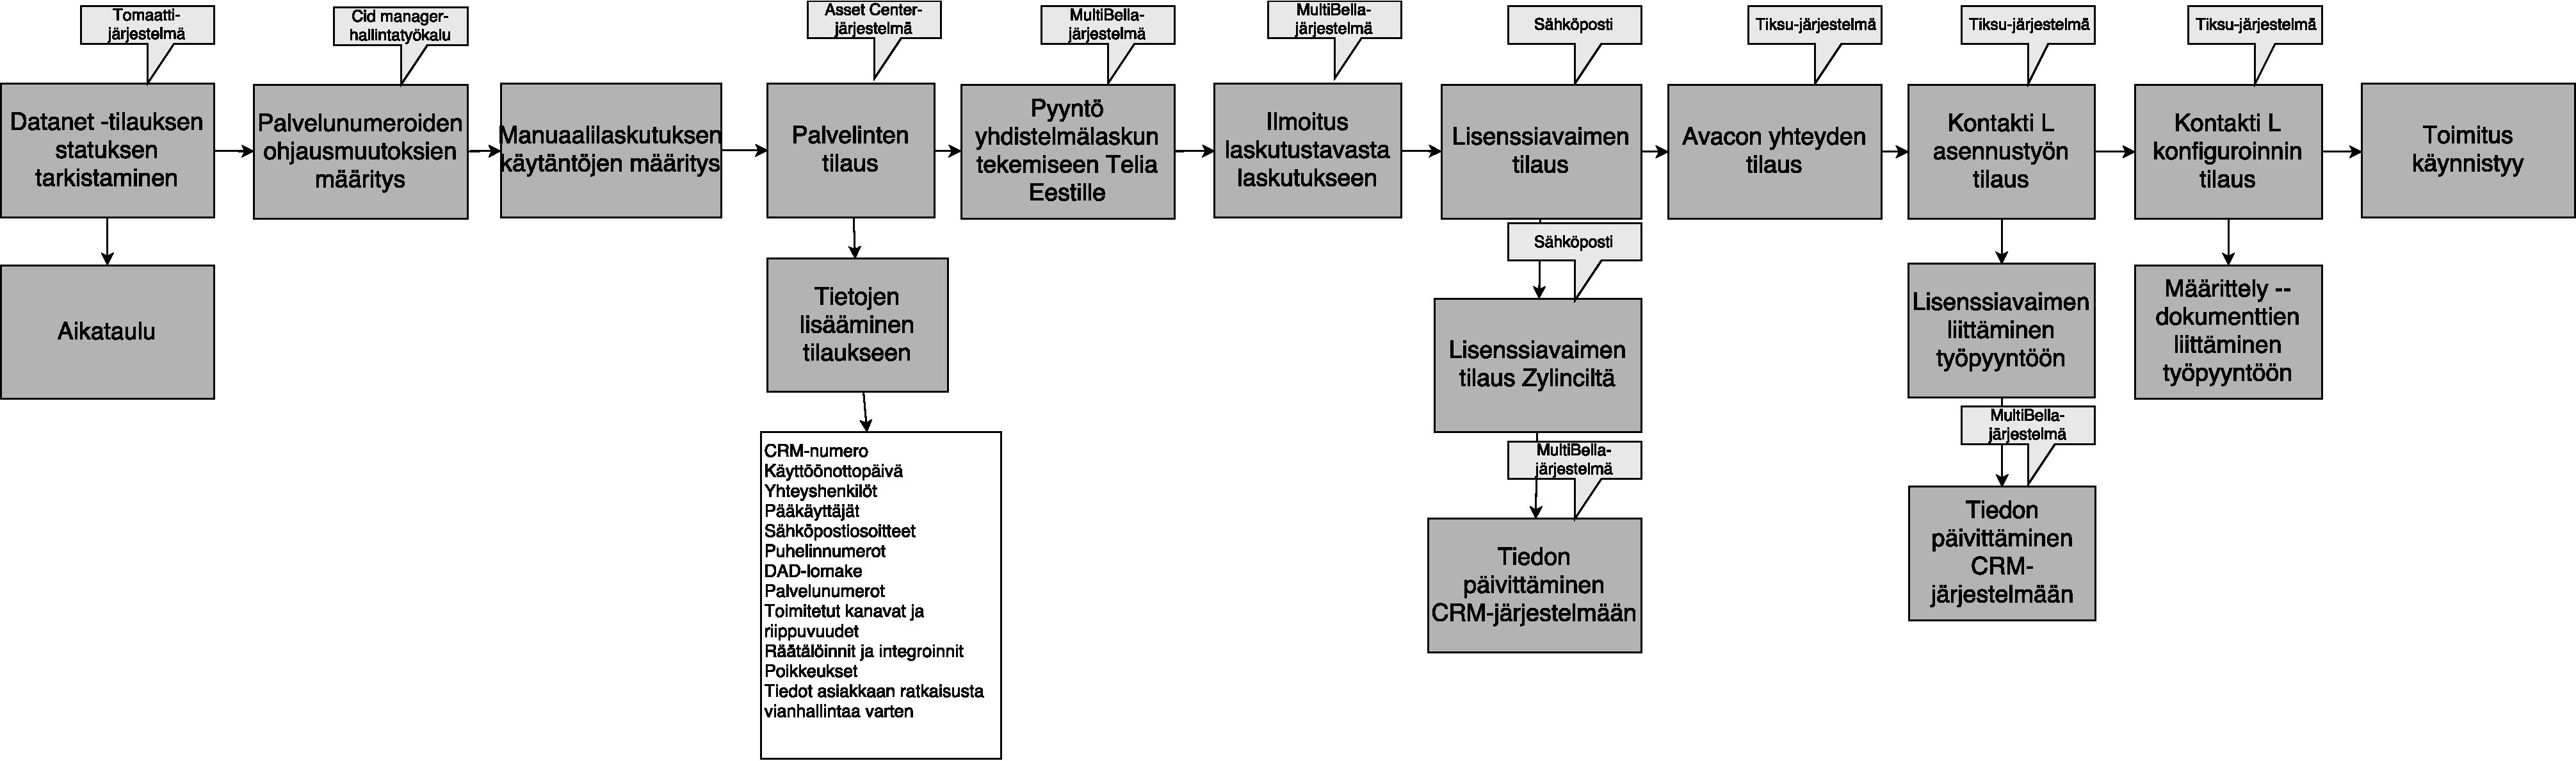
\includegraphics[scale=0.2]{images/valmtoimlask.pdf}
    \caption{Kontakti L:n asiakasprosessin suunnitteluvaiheen toimituksen ja laskutuksen valmistelu.}
    \label{fig:valmtoimlask}
\end{figure}

Ensimmäinen toimitusvastaavan tehtävä on seurata Datanet-yhteyksien toimitusta ja saada aikataulu sen valmistumisesta, koska toimitusvaihe ei voi alkaa ennen yhteyksien saamista. Tämän jälkeen hän tekee asiakkaan palvelunumeroista ohjausmääritykset valmiiksi Cid manager numeroiden hallintatyökalun kautta odottamaan toimitusta. Toimitusvastaava käy myös seuraavaksi läpi manuaalilaskutuksen käytännöt Kontakti L:n tuotepäällikön kanssa, että hänellä on tarvittavat tiedot laskutustavasta ja yhdistelmälaskun tilaamisesta asiakkaalle.\\

Tämän jälkeen toimitusvastaava tilaa Kontakti L:n palvelimet Asset Center-järjestelmästä, ja lisää tietoihin kuvassa näkyvät tiedot asiakkaan ratkaisusta vianhallintaa varten. Sitten hän tekee MultiBella-järjestelmässä työpyynnön Telia Eestille yhdistelmälaskun tekemisestä asiakkaalle ja ilmoittaa laskutustavan Suomen laskutukseen.\\

Seuraavaksi toimitusvastaava pyytää sähköpostitse Kontakti L:n tuotekehityspäällikköä tilaamaan lisenssiavaimen järjestelmään Zylinciltä ja päivittää tiedon tästä MultiBella-järjestelmään. Tuotekehityspäällikkö tilaa lisenssiavaimen sähköpostitse Zylinciltä. Palvelinten ollessa valmiina, toimitusvastaava tilaa Tiksu tiketöintijärjestelmästä etäyhteydet toimitusta varten. Etäyhteyksien toimiessa, hän lähettää Tiksu-järjestelmästä työpyynnön Tiedolle Kontakti L:n asennusta varten ja liittää sähköpostista lisenssiavaimen liitteeksi.\\

Kun Tieto on kuitannut asennuksen valmistuneen, päivittää toimitusvastaava tiedon Multibella-järjestelmään. Seuraavaksi hän tilaa Kontakti L:n konfigurointi ja integrointityön Telian järjestelmäasiantuntijalta Tiksu-järjestelmän kautta ja liittää määrittelydokumentit työpyynnön liitteeksi.\\

Toimitusvastaava seuraa työvaiheiden toteutumista ja päivittää tiedot MultiBella-järjestelmään. Tämä seuranta kuuluu osaltaa jo seuraavaan toimitusvaiheeseen asiakasprosessia.\\

\textbf{Toimitusvaihe}\\

Vaiheen kesto on arvioitu olevan noin 2-4 kuukautta.\\

Tämä vaihe on esitetty kuvassa \ref{fig:toimitus}. (Ei toistaiseksi tarkempaa tietoa yhteyksien toimituksesta) Toimitusvaihe alkaa kun Datanet-toimitus saa Tiksu-järjestelmästä työpyynnön yhteyksien toimittamisesta. Työpyynnön liitteenä on IP-suunnittelijan tekemä verkkokuva, jonka perusteella yhteydet toimitetaan. Työn valmistuessa asiantuntija kuittaa Tiksu-järjestelmän työpyynnön valmiiksi.\\

\begin{figure}[!h]
    \centering
    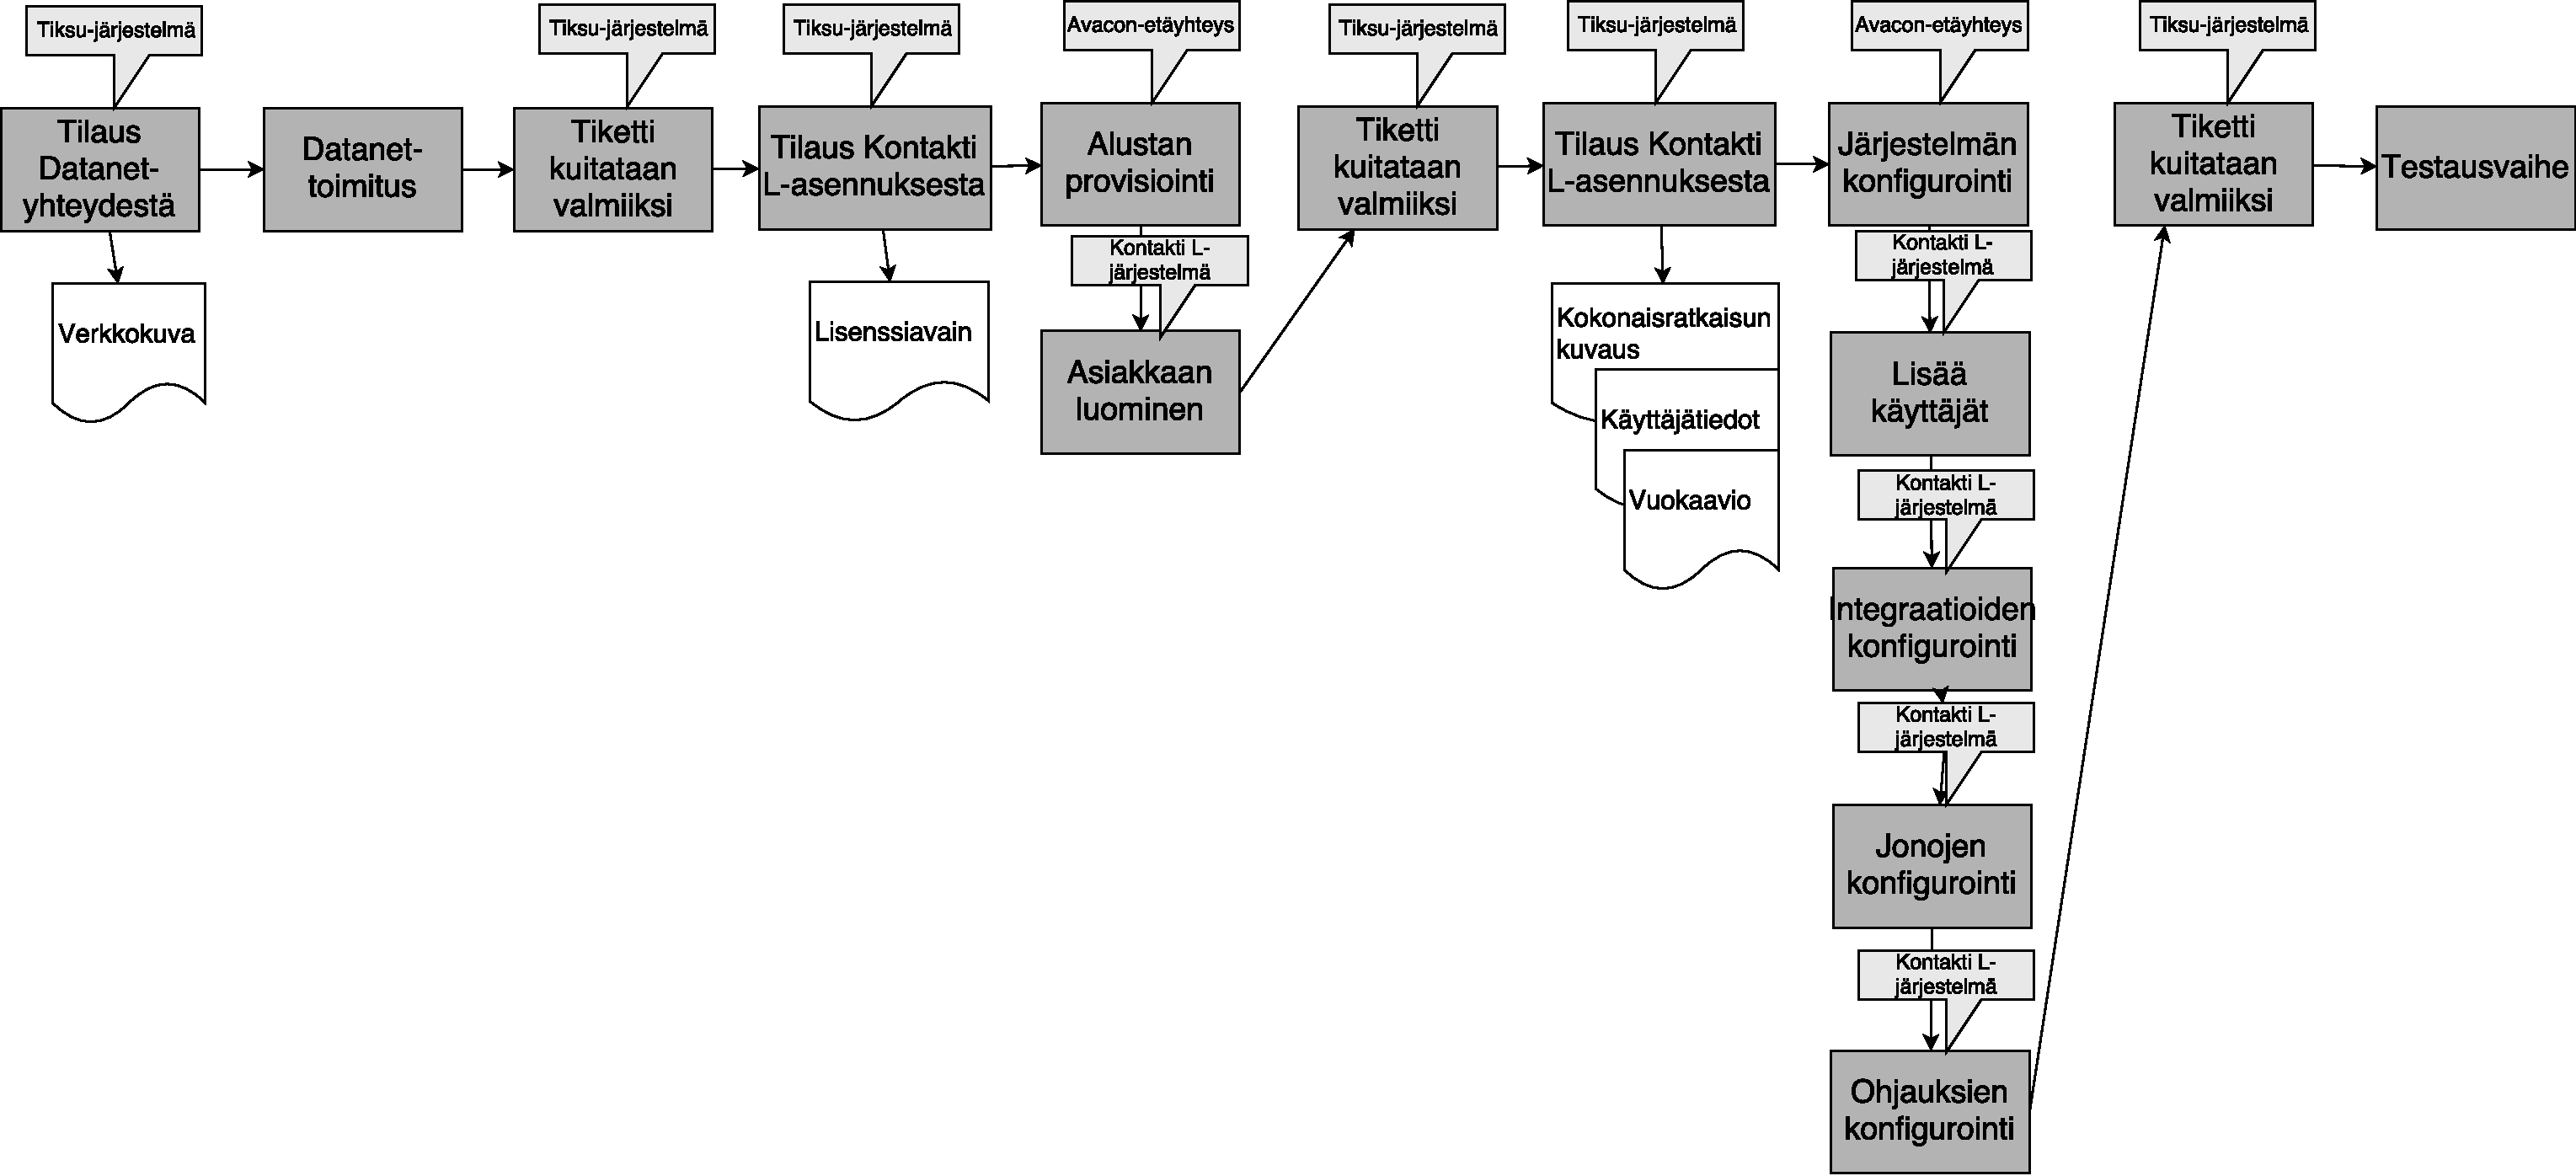
\includegraphics[scale=0.3]{images/toimitus.pdf}
    \caption{Kontakti L:n asiakasprosessin toimitusvaihe.}
    \label{fig:toimitus}
\end{figure}

Tämän jälkeen Tiedon järjestelmäasiantuntija saa työpyynnön Tiksu-järjestelmässä Kontakti L:n asennuksesta, jonka liitteenä on järjestelmän lisenssiavain. Järjestelmäasiantuntija asentaa Kontakti L:n palvelimelle Avacon-etäyhteyden avulla, ja kuittaa tämän jälkeen työpyynnön valmiiksi Tiksu-järjestelmässä.\\

Tämän jälkeen Telian järjestelmäasiantuntija saa työpyynnön Tiksu-järjestelmässä Kontakti L:n konfigurointi- ja integrointityöstä. Työpyynnön liitteenä on ratkaisun määrittelydokumentit ja käyttäjätiedot. Järjestelmäasiantuntija ottaa Avacon-etäyhteyden Kontakti L-palvelimelle. Ensin hän lisää käyttäjätiedon Kontakti L-järjestelmään, ja sen jälkeen tekee tarvittavat integroinnit. Kun integraatiot toimivat, alkaa järjestelmäasiantuntija konfiguroimaan jonoja ja kontaktien ohjaustietoja järjestelmään. Kun kaikki integraatiot ja konfiguroinnit on todettu toimiviksi, järjestelmäasiantuntija kuittaa Tiksu-järjestelmän työpyynnön valmiiksi.\\

Tämän jälkeen alkaa Kontakti L-järjestelmän testausvaihe.\\

\textbf{Testausvaihe}\\

Tästä vaiheesta ei ole ohjeistusta tai dokumentaatiota. Haastatteluissa Telian järjestelmäasiantuntija kertoi testanneensa järjestelmän toimintaa integrointi ja konfigurintivaiheessa.\\

\textbf{Koulutusvaihe}\\

Kuvassa \ref{fig:koulutus} ilmenee koulutusvaiheen kulku. Koulutusvaihe alkaa kun kouluttaja käy sopimuksen läpi projektipäällikön tai toimitusvastaavan kanssa. Asiakkaan kanssa tehdystä sopimuksesta ilmenee mitä koulutuksista on sovittu asiakkaan kanssa.

\begin{figure}[!h]
    \centering
    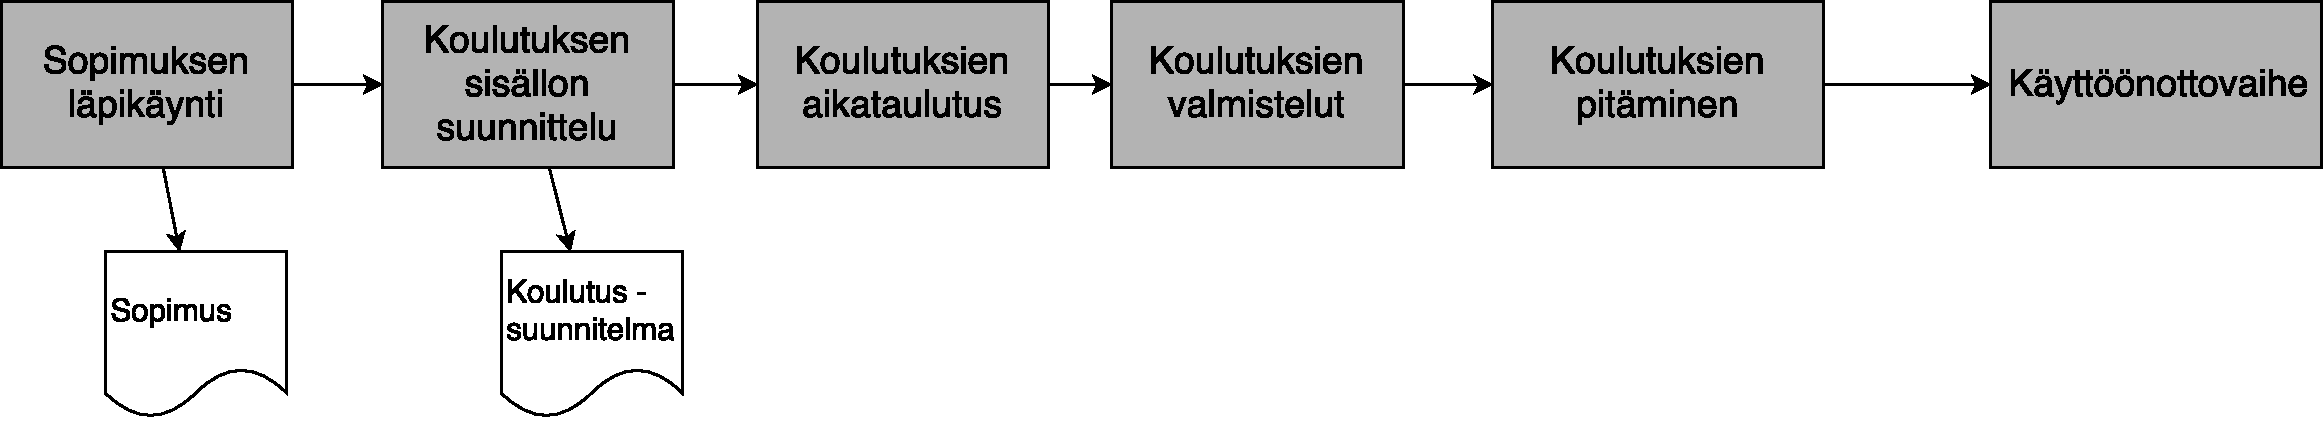
\includegraphics[scale=0.3]{images/koulutukset.pdf}
    \caption{Kontakti L:n asiakasprosessin koulutusvaihe.}
    \label{fig:koulutus}
\end{figure}

Sopimuksen perusteella kouluttaja suunnittelee koulutuksen sisällön ja tekee tästä kirjallisen suunnitelman. Koulutuksen sisällön ollessa selvillä, aikatauluttaa kouluttaja yhdessä projektipäällikön ja toimitusvastaavan kanssa tarvittavien koulutusten ajankohdan.\\

Kouluttaja tyypillisesti valmistelee koulutusta asiakkaan tarpeen mukaan, ja koulutus voidaan järjestää joko Telian tiloissa tai asiakkaalla. Kouluttaja pitää koulutukset suunnitelman mukaan. Järjestelmän käyttäjien ollessa valmiita ottamaan järjestelmä jokapäiväiseen käyttöön, alkaa käyttöönottovaihe.\\

\textbf{Käyttöönottovaihe}\\

\textbf{Lopetusvaihe}\\

\textbf{Laskutusvaihe}\\

\subsubsection{Esiin nousseet haasteet}

Prosessin rakennusvaiheen haasteet tavoitejärjestelmien ja vendorin osalta.


Käyttöönoton ongelmat usein joko lisäpalveluiden käyttöönoton haasteita tai ohjeiden epäselvyyksiin liittyviä. 


\textbf{Tilausvaiheessa esiin nousseet haasteet}\\

- Myyjä ei osaa täyttää paha-lomaketta ja jättää sen usein tekemättä\\
- Myyjällä ei ole tällöin tapaa viestiä siitä minkä palvelun hän on myynyt\\
- Myyjän on haastava viestiä eteenpäin mitä hän on myynyt\\

\textbf{Tilausten vastaanotto-vaiheessa esiin nousseet haasteet}\\

- Vaiheen läpi pääsee ilman PaHa-lomaketta, jolloin asiantuntijan täytyy selvittää joko myynnistä, projektitoimistolta tai tuotehallinnalta mitä tilaukselle tehdään.\\

Zylincin pystyttämisen automatisointi. Tilausvaiheen lomakkeet, myyjän vastuu, 

ODI-prosessin kuvaus.

Haettiin Ruotsin CallGuidea selkeästi halvempaa ja kevyempää IMS-yhteensopivaa ratkaisua, jolla voidaan korvata Merex/Mecm vaihteenhoitopalvelu ja kasvattaa markkinaosuutta ns. keskisegmentissä (joitain kymmeniä agentteja). Projekti taisi alkaa 2015 ja sopimusneuvotteluiden jälkeen tuotteistus/asiakasprosessin rakentaminen alkoi 2017 kesällä. Pilotoitiin kuitenkin jostain syystä yli sadan agentin asiakkaalla, jolla tuhansia kontakteja viikossa. Pilotti alkoi yli vuosi sitten ja teknisistä ongelmista johtuen laskutus ei ole alkanut vieläkään. Selkeästi halvemman hinnan ansiosta voitettu isoja toimijoiden kilpailutuksia. Useita alkuperäiseen haarukkaan kuuluneita asiakkaita jonossa, mutta toimitukset venyvät kaiken ajan kuluessa isojen toimitusten virittämiseen.

\subsection{Kappaleen yhteenveto}


\clearpage

\section{Havainnot}
%\section{Results}


%% Huomaa seuraavassa kappaleessa lainausmerkkien ulkopuolella piste, 
%% koska piste ei lopeta lainattua tekstinpätkää.
%% Jos lainattu tekstinpätkä loppuu välimerkkiin, tulee välimerkki
%% lainausmerkkien sisälle: 
%% "Et tu, Brute?" sanoi Caesar kuollessaan.
Tutkimustuloksien merkitystä on aina syytä arvioida ja tarkastella
kriittisesti.  Joskus tarkastelu voi olla tässä osassa, mutta se
voidaan myös jättää viimeiseen osaan, jolloin viimeisen osan nimeksi
tulee >>Tarkastelu>>. Tutkimustulosten merkitystä voi arvioida myös
>>Johtopäätökset>>-otsikon alla viimeisessä osassa. 

Tässä osassa on syytä myös arvioida tutkimustulosten luotettavuutta.
Jos tutkimustulosten merkitystä arvioidaan >>Tarkastelu>>-osassa,
voi luotettavuuden arviointi olla myös siellä. 

\clearpage

\section{Tutkimuskysymyksiin vastaaminen}

\section{Yhteenveto}
%\section{Summary} 

Opinnäytteen tekijä vastaa siitä, että opinnäyte on tässä dokumentissa
ja opinnäytteen tekemistä käsittelevillä luennoilla sekä
harjoituksissa annettujen ohjeiden mukainen muotoseikoiltaan,
rakenteeltaan ja ulkoasultaan.



\clearpage
%% Lähdeluettelo
%%
%% \phantomsection varmistaa, että hyperref-paketti latoo hypertekstilinkit
%% oikein.
%%
%% The \phantomsection command is nessesary for hyperref to jump to the 
%% correct page, in other words it puts a hyper marker on the page.

\phantomsection
%\addcontentsline{toc}{section}{Viitteet}
%\addcontentsline{toc}{section}{References}
%%\begin{thebibliography}{99}
\bibliography{lahteet}

%% Alla pilkun jälkeen on pakotettu oikea väli \<välilyönti>-merkeillä.

%%\end{thebibliography}

%% Liitteet 
\appendix 
\clearpage
%% Lisää tekstin "Liitteet" sisällysluetteloon
%%
%% Adds the word "Appendices" to the table of contents
\addtocontents{toc}{\protect\contentsline{section}{Liiteet}{}{appendix}}
%\addtocontents{toc}{\protect\contentsline{section}{Appendices}{}{appendix}}

\section{Esimerkki liitteestä\label{LiiteA}}
%% Liitteiden kaavat, taulukot ja kuvat numeroidaan omana kokonaisuutenaan
%%
%% Equations, tables and figures have their own numbering in Appendices
\renewcommand{\theequation}{A\arabic{equation}}
\setcounter{equation}{0}  
\renewcommand{\thefigure}{A\arabic{figure}}
\setcounter{figure}{0}
\renewcommand{\thetable}{A\arabic{table}}
\setcounter{table}{0}

Liitteet eivät ole opinnäytteen kannalta välttämättömiä ja 
opinnäytteen tekijän on 
kirjoittamaan ryhtyessään hyvä ajatella pärjäävänsä ilman liitteitä.
Kokemattomat kirjoittajat, jotka ovat huolissaan
tekstiosan pituudesta, paisuttavat turhan 
helposti liitteitä pitääkseen tekstiosan pituuden annetuissa rajoissa.
Tällä tavalla ei synny hyvää opinnäytettä.   

Liite on itsenäinen kokonaisuus, vaikka se täydentääkin tekstiosaa.
Liite ei siten ole pelkkä listaus, kuva tai taulukko, vaan 
liitteessä selitetään aina sisällön laatu ja tarkoitus. 

Liitteeseen voi laittaa esimerkiksi listauksia. Alla on 
listausesimerkki tämän liitteen luomisesta. 

%% Verbatim-ympäristö ei muotoile tai tavuta tekstiä. Fontti on monospace.
%% Verbatim-ympäristön sisällä annettuja komentoja ei LaTeX käsittele. 
%% Vasta \end{verbatim}-komennon jälkeen jatketaan käsittelyä.
\begin{verbatim}
	\clearpage
	\appendix
	\addcontentsline{toc}{section}{Liite A}
	\section*{Liite A}
	...
	\thispagestyle{empty}
	...
	tekstiä
	...
	\clearpage
\end{verbatim}

Kaavojen numerointi muodostaa liitteissä oman kokonaisuutensa:
\begin{eqnarray}
d \wedge A  &=& F, \label{liitekaava1}\\
d \wedge F  &=& 0. \label{liitekaava2}
\end{eqnarray}


\clearpage
\section{Toinen esimerkki liitteestä\label{LiiteB}}

%% Liitteiden kaavat, taulukot ja kuvat numeroidaan omana kokonaisuutenaan
%%
%% Equations, tables and figures have their own numbering in Appendices
\renewcommand{\theequation}{B\arabic{equation}}
\setcounter{equation}{0}  
\renewcommand{\thefigure}{B\arabic{figure}}
\setcounter{figure}{0}
\renewcommand{\thetable}{B\arabic{table}}
\setcounter{table}{0}

Liitteissä voi myös olla kuvia, jotka
eivät sovi leipätekstin joukkoon:
%% Ympäristön figure parametrit htb pakottavat
%% kuvan tähän, eikä LaTeX yritä siirrellä niitä
%% hyväksi katsomaansa paikkaan. 
%% Ympäristöä center voi käyttää \centering-
%% komennon sijaan
%%
%% Example of a figure, note the use of htb parameters which force
%% the figure to be inserted here
\begin{figure}[htb]
\begin{center}
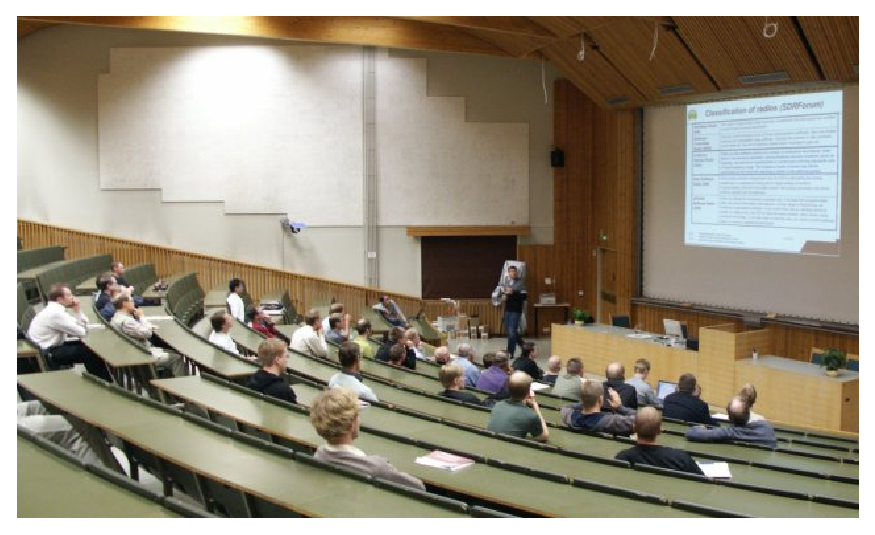
\includegraphics[height=8cm]{kuva2}
\end{center}
\caption{Kuvateksti, jossa on liitteen numerointi \label{liitekuva}}
\end{figure}
%%
Liitteiden taulukoiden numerointi on kuvien ja kaavojen kaltainen:
\begin{table}[htb]
\caption{Taulukon kuvateksti. \label{liitetaulukko}}
\begin{center}
\fbox{
\begin{tabular}{lp{0.5\linewidth}}
9.00--9.55  & Käytettävyystestauksen tiedotustilaisuus (osanottajat
ovat saaneet sähköpostitse valmistautumistehtävät, joten tiedotustilaisuus
voidaan pitää lyhyenä).\\
9.55--10.00 & Testausalueelle siirtyminen
\end{tabular}}
\end{center}
\end{table}
Kaavojen numerointi muodostaa liitteissä oman kokonaisuutensa:
\begin{eqnarray}
T_{ik} &=& -p g_{ik} + w u_i u_k + \tau_{ik},  \label{liitekaava3} \\
n_i    &=& n u_i + v_i.                        \label{liitekaava4}
\end{eqnarray}

\end{document}
